% ============================================================
%  Invisible Watermarking for AI-Generated Images
%  Replicating and Extending Tree-Ring Watermarks
%  GNN for the Sciences -- University of Heidelberg WS 2025/26
%  IEEE Two-Column Layout
% ============================================================
\documentclass[10pt,twocolumn]{article}


%-- IEEE-like page geometry (manual, no geometry package) --%
\setlength{\oddsidemargin}{-0.04cm}
\setlength{\evensidemargin}{-0.04cm}
\setlength{\textwidth}{17.2cm}
\setlength{\columnsep}{0.6cm}
\setlength{\topmargin}{-0.54cm}
\setlength{\headheight}{0pt}
\setlength{\headsep}{0pt}
\setlength{\textheight}{24.7cm}

\usepackage{graphicx}
\usepackage{times}
\usepackage{amsmath}
\usepackage{amssymb}
\usepackage{bm}
\usepackage{booktabs}
\usepackage{multirow}
\usepackage{array}
\usepackage{url}
\usepackage{xcolor}
\usepackage{subcaption}
\usepackage{tikz}
\usetikzlibrary{arrows.meta,positioning,shapes.geometric,calc}
\usepackage[pdftex,colorlinks=true,citecolor=blue,urlcolor=blue,linkcolor=black]{hyperref}

%-- IEEE-style section headings --%
\makeatletter
\renewcommand\section{\@startsection{section}{1}{\z@}%
  {-2.5ex \@plus -1ex \@minus -.2ex}{1.0ex \@plus .2ex}%
  {\normalfont\normalsize\bfseries\MakeUppercase}}
\renewcommand\subsection{\@startsection{subsection}{2}{\z@}%
  {-2.0ex \@plus -1ex \@minus -.2ex}{0.5ex \@plus .2ex}%
  {\normalfont\normalsize\itshape}}
\renewcommand\subsubsection{\@startsection{subsubsection}{3}{\z@}%
  {-1.5ex \@plus -0.5ex \@minus -.2ex}{0.3ex \@plus .2ex}%
  {\normalfont\normalsize\bfseries}}
\makeatother

%-- Colour helpers --%
\definecolor{passgreen}{HTML}{1B5E20}
\definecolor{warnamber}{HTML}{E65100}
\definecolor{failred}{HTML}{B71C1C}
\newcommand{\pass}[1]{\textcolor{passgreen}{\textbf{#1}}}
\newcommand{\warn}[1]{\textcolor{warnamber}{#1}}
\newcommand{\fail}[1]{\textcolor{failred}{#1}}

%-- Math shortcuts --%
\newcommand{\F}{\mathcal{F}}
\newcommand{\E}{\mathcal{E}}
\newcommand{\D}{\mathcal{D}}

\pagestyle{plain}
\pagenumbering{arabic}

% ============================================================

\begin{document}

% ---------------- FRONT PAGE ----------------
\begin{titlepage}
    \centering
    
    \vspace*{2cm}
    
    {\LARGE \textbf{Invisible Watermarking for AI-Generated Images: Replicating and Extending Tree-Ring Watermarks with Dual-Band and All-Channel Fourier Embedding}\par}
    
    \vspace{2cm}
    
    {\large
    Ashhad Raza Quadri\\
    Matriculation Number: 4756039\\[0.5cm]
    Maria Alejandra Pabon Galindo\\
    Matriculation Number: 4756044\\[0.5cm]
    Saliq\\
    Matriculation Number: 11111
    \par}
    
    \vspace{2.5cm}
    
    {\large
    \textbf{Repository:} \\
    \url{https://github.com/Ashhad1130/Invisible_Watermark_GNN}
    \par}
    
    \vspace{2.5cm}
    
    {\large
    \textit{Generative Neural Networks for the Sciences,
    Winter Semester 2025/26,
    Ruprecht-Karls-Universit\"at Heidelberg.}
    \par}
    
    \vspace{3cm}
    
    {\large
    \textbf{Submitted:} March 30, 2026
    \par}
    
    \vfill
\end{titlepage}

\onecolumn

\noindent\hrulefill\vspace{4pt}

\noindent\textbf{Abstract---}
The mass deployment of latent diffusion models (LDMs) for text-to-image
synthesis has created an urgent need for reliable, scalable content
provenance mechanisms.
We study, replicate, and extend
\emph{Tree-Ring Watermarking}~\cite{wen2023treering},
a training-free method that embeds an invisible ring-shaped fingerprint
into the Fourier spectrum of the initial diffusion noise latent,
making the watermark inseparably entangled with the generated image
through the entire deterministic DDIM denoising trajectory.
Starting from a paper-exact baseline replication --- 50 DDIM steps,
single Fourier channel, circular ring mask, AUC matching Wen et al.\
within $\pm$0.01 on all seven reported attacks --- we design and evaluate
three progressive improvements grounded in the frequency-domain
theory of diffusion model inversion:
(1)~\textbf{Step Optimisation} --- doubling DDIM inversion steps
from 50 to 100, reducing reconstruction error as $\mathcal{O}(1/N)$
and improving the Fourier match to the embedded key;
(2)~\textbf{Dual-Band Multi-Ring Masking} --- a theoretically motivated
two-band Fourier mask combining an inner low-frequency disc
($\rho \le 4$) and an outer ring ($6 \le \rho \le 10$), providing
spectral redundancy across two complementary frequency regions;
and (3)~\textbf{All-Channel Embedding} --- extending watermark injection
from one to all four latent channels, improving signal-to-noise ratio
by approximately $2\times$ under phase-disrupting geometric attacks.
We evaluate on 50 generated images across 8 semantic categories
and 13 distinct attack conditions, reporting AUC, balanced accuracy,
and the deployment-critical TPR@1\%FPR metric.
Our best configuration, \emph{MR-AllChan}, achieves AUC $\geq 0.97$
on 12/13 attacks, resolves all five FAIL conditions of the baseline,
and surpasses the paper's reported crop\_0.75 AUC (0.996 vs.\ 0.97).
The improvement over the baseline is statistically significant
(Wilcoxon signed-rank, $p{=}0.012$) across all 13 attack conditions.
We further show that all-channel embedding reduces perceptual similarity
between watermarked and unwatermarked outputs (pHash: $0.58$ vs.\ $0.77$
for single-channel), quantifying the robustness--imperceptibility
trade-off inherent to source-side Fourier watermarking.
We provide mechanistic analysis through per-image L1 score distributions,
actual ROC curves from real checkpoint data, ablation studies, and a
frequency-domain theoretical analysis explaining the success and limits
of each modification.

\vspace{6pt}
\noindent\textbf{Index Terms---}
invisible watermarking, latent diffusion models, DDIM inversion,
Fourier fingerprinting, Tree-Ring, dual-band spectral embedding,
all-channel embedding, image provenance, AI-generated content detection,
robustness evaluation.

\vspace{6pt}\noindent\hrulefill\vspace{8pt}

\newpage

% ============================================================
%-- Table of Contents (required by guidelines) --%
{\onecolumn\tableofcontents\twocolumn}

% ============================================================

% ---------------- ABSTRACT ----------------


\section{Introduction}
\label{sec:intro}
\textit{Main contributors: Ashhad Raza Quadri, Maria Alejandra Pabon.}


The capacity of modern generative models to synthesize photorealistic
images has grown dramatically over the past five years.
Latent diffusion models (LDMs) such as Stable Diffusion
~\cite{rombach2022ldm} and Imagen~\cite{saharia2022imagen}
can now produce images that are indistinguishable from photographs in
blind human evaluations, with creative quality rivaling or surpassing
professional photographers and artists in many domains.
This can be done  with just a natural language prompt that describes 
what you want to see in the image, thereby narrowing the gap between
language and vision~\cite{fan2025trustworthiness}.
Generative AI can 
ne used to improve effectiveness, efficiency, and creativity
in various activities such as image generation, image super-resolution, 
image inpainting, or image editing~\cite{10081412}.
This capability, while transformative for legitimate creative industries,
simultaneously enables a range of harmful applications.
Deepfake videos of political figures have been used to influence
elections; fabricated scientific imagery has appeared in peer-reviewed
publications; non-consensual intimate synthetic imagery has been weaponized
for harassment; and misinformation campaigns now use AI-generated
photographs as apparent visual evidence. Furthermore, AI-generated images
can be misused in more subtle but widespread ways: individuals may falsely
claim generated content as their own work, students may rely on such images
to complete or assist with academic assignments or assessments, and users
may distribute synthetic content while asserting ownership or copyright
~\cite{jiang2023evading}.

The regulatory response has been swift and global.
The European Union's AI Act (effective August 2024) mandates disclosure
of AI-generated content in Article~52, requiring that AI systems
producing synthetic images label them as such, with non-compliance
penalties of up to 3\% of global annual turnover.
The United States Executive Order on Trustworthy Artificial Intelligence
(October 2023) directed federal agencies to develop standards for digital
watermarking and content provenance within one year.
The Coalition for Content Provenance and Authenticity (C2PA) standard
is now being adopted by Adobe, Microsoft, Google, and major news
organisations to attach cryptographic provenance metadata to media at
creation time.
In China, the Provisions on the Management of Deep Synthesis Internet
Information Services (2023) similarly mandate watermarking of
AI-generated content at the service provider level.

Against this backdrop, reliable, invisible, and robust watermarking
of AI-generated images is both a technical challenge and a pressing
societal necessity.

\subsection{Technical Context}

Modern text-to-image generation is predominantly based on the
\textit{diffusion model} paradigm. Diffusion models are a class of deep
generative models that synthesise data by learning to reverse a gradual
noising process: an input is progressively corrupted with Gaussian noise,
and a neural network is trained to iteratively denoise
this signal to recover realistic samples (reverse process)
~\cite{10081412}. In practice, efficient image generation often relies
on DDIM sampling, which provides a faster and partially deterministic
alternative to standard stochastic diffusion sampling
~\cite{song2021denoising}.

Within this framework, \textit{watermarking} aims to embed an
imperceptible signal into generated images in order to enable reliable
attribution of their origin. An effective watermark must remain visually
undetectable while being robust to common image transformations such as
compression, cropping, or geometric distortions~\cite{NEURIPS2024}.
Unlike traditional post-processing approaches, diffusion-based methods
allow watermark signals to be incorporated directly into the generation
process, enabling stronger coupling between the watermark and the image
content.

A representative approach in this setting is \textit{source-side
watermarking}, where the signal is embedded not in the final image but
in the generative process itself. In diffusion models, this can be
achieved by modifying the \emph{initial noise latent} that seeds the
generation trajectory. Because the entire image is derived from this
latent through iterative denoising, any structured signal embedded in it
can propagate through the process and become implicitly encoded in the
final output. However, watermarking diffusion models is inherently challenging.
The stochastic nature of generation, the high-dimensional latent space,
and the sensitivity of inversion procedures make it difficult to design
signals that are both robust and reliably detectable.


\subsection{The Technical Challenge of Source-Side Watermarking}

The core technical problem appears deceptively simple: \emph{given an
image, can we reliably determine whether it was generated by a
particular AI system?}
A naive approach --- appending a visible watermark logo to generated
images --- is trivially defeated by cropping.
\emph{Post-hoc} invisible watermarking --- modifying finished pixel
values to embed a signal --- is more sophisticated but has two
fundamental weaknesses that are particularly severe for diffusion models.

First, the adversary can simply regenerate the image from a different
random seed to obtain a clean, unmarked copy with similar content.
For diffusion models, the generation process is stochastic: changing
the initial noise seed $z_T$ by a single bit produces a completely
different image that contains no trace of the watermark.
This \emph{regeneration attack} entirely circumvents post-hoc
watermarking.

Second, even without regeneration, post-hoc invisible watermarks are
fragile under common image processing.
JPEG compression at quality factor 25 (a common social media setting)
removes most LSB-based watermarks.
Geometric transformations such as rotation, crop, or scaling, misalign the
watermark pattern with any fixed reference grid.
Colour adjustments change pixel-level statistics.
Each of these operations is a routine, non-adversarial post-processing
step in the image distribution pipeline.

\emph{Source-side} watermarking addresses both weaknesses by modifying
the \emph{generation process} itself rather than post-processing the
output.
Every image produced by a specific model instance automatically carries
a fingerprint that is intrinsically tied to the image content through
the generative process rather than appended to it.
For diffusion-based generators, source-side watermarking is the only
principled approach that survives regeneration attacks, since the
fingerprint is encoded in the generation seed rather than the pixels.

\subsection{Tree-Ring: Source-Side Watermarking for Diffusion Models}

Wen et al.~\cite{wen2023treering} introduced Tree-Ring Watermarking,
which exploits a fundamental structural property of DDIM
generation~\cite{song2020ddim}: given a fixed initial noise latent
$z_T$, the generated image is \emph{uniquely and deterministically}
determined.
The method embeds a secret ring-shaped pattern into the Fourier domain
of $z_T$ before generation begins (Fig.~\ref{fig:pipeline}).
Because the entire denoising trajectory is seeded by the modified
latent, the watermark signature propagates into every pixel through
the diffusion process, without any post-hoc modification.
The watermark is thus not an additive overlay but an intrinsic property
of the generation trajectory: an image with the watermark embedded in
its seed cannot be ``de-watermarked'' without fundamentally changing
the image content.

At detection time, DDIM inversion --- running the approximate forward
diffusion process on the suspected image --- recovers an estimate
$\tilde{z}_T \approx z_T$.
The detector then checks whether the ring pattern is present in the
Fourier spectrum of the recovered noise.
No reference image, generation prompt, or model-specific knowledge is
needed at detection time: the detector operates completely blindly,
requiring only the secret ring pattern key.

The original paper reports AUC above 0.97 on all seven evaluated
attacks (Table~2 of~\cite{wen2023treering}) on Stable Diffusion v2.1.
The method is elegant in its simplicity: it requires no model
modification, no additional training, and no change to the generation
interface visible to users.

\subsection{Limitations of the Original Work}

Despite its strong reported results, we identify three specific
limitations of the original work that motivate our extensions:

\begin{enumerate}
  \item \textbf{Limited attack coverage.}
    The evaluation covers only 7 attack conditions: no\_attack,
    gaussian\_blur\_8, jpeg\_25, brightness\_6, gaussian\_noise\_0.1,
    crop\_0.75, and rotation\_75.
    Importantly, this omits several natural attack intensifications
    (50\% crop, 45$^\circ$ rotation, JPEG quality 25, stronger noise),
    leaving the robustness profile incomplete for deployment decisions.

  \item \textbf{Single-channel embedding.}
    Embedding the watermark in only one of the four latent channels
    ($c{=}3$) leaves three channels of signal capacity completely unused.
    Under attacks that introduce systematic phase distortions in the
    Fourier domain (such as rotation), single-channel detection is
    sensitive to the specific Fourier phase structure of the chosen
    channel and has high per-image score variance.

  \item \textbf{Single-band mask.}
    The narrow circular mask at radius $r = 10$ concentrates the
    watermark in one frequency band.
    Under spatial truncation (crop), energy at $r = 10$ is redistributed
    across neighbouring frequencies by a sinc-type convolution, substantially
    weakening the watermark signal.
    A multi-band design could provide spectral redundancy: different bands
    can survive different classes of attacks.
\end{enumerate}

\subsection{Our Contributions}

This paper makes five concrete contributions:

\begin{enumerate}
  \item \textbf{Paper-accurate replication.}
    We reimplement Tree-Ring Watermarking from scratch using Stable
    Diffusion v1.5 and reproduce all seven AUC values from Table~2 of
    Wen et al.~\cite{wen2023treering} within $\pm$0.01, validating our
    implementation pipeline.

  \item \textbf{Step-count optimisation with theoretical justification.}
    We provide a formal $\mathcal{O}(1/N)$ reconstruction error bound
    (Eq.~\ref{eq:euler_error}) and empirically verify the benefit of
    increasing DDIM inversion steps from $N{=}50$ to $N{=}100$.

  \item \textbf{Dual-band multi-ring mask.}
    We design a two-band Fourier mask motivated by frequency-domain
    analysis of crop and blur attacks, with a calibrated spectral gap
    ($r_{\mathrm{in}}{=}4$, $r_{\mathrm{out}}{=}10$, $g{=}2$),
    and verify its optimality through an inner-radius ablation study.

  \item \textbf{All-channel embedding.}
    We extend watermark injection and detection to all four latent
    channels, providing $\sqrt{4} = 2\times$ SNR under phase-noise
    attacks. We verify the per-channel contribution through a channel
    subset ablation study.

  \item \textbf{Extended evaluation on 13 attacks with mechanistic analysis.}
    We provide AUC, accuracy, and TPR@1\%FPR across 13 attack conditions
    (6 more than the paper), actual ROC curves from real per-image
    checkpoint data, score distribution histograms, and a mechanistic
    explanation of why each modification succeeds or fails.
\end{enumerate}

\subsection{Research Questions}

\textbf{RQ1} \textit{(Replication):}
Does our implementation reproduce the AUC values of Wen et al.\
within $\pm$0.01 on all seven paper-reported attacks?

\textbf{RQ2} \textit{(Step Optimisation):}
Does increasing DDIM inversion steps from 50 to 100 uniformly improve
detection accuracy across all attack types, and if not, what determines
where it helps and where it hurts?

\textbf{RQ3} \textit{(Structural Innovation):}
Does the combination of a dual-band Fourier mask and all-channel
embedding resolve all baseline failure cases on crop and rotation
attacks, and are the two modifications synergistic?

For RQ1 reproducibility is a necessary condition for
any meaningful extension: if the baseline cannot be reproduced
faithfully, later improvements cannot be interpreted correctly.
For RQ2 DDIM inversion is the core mechanism underlying
detection, and its numerical accuracy may directly affect robustness.
However, its effect is difficult to predict in advance, since more
accurate inversion may improve recovery of the watermark signal while
also more faithfully reconstructing attack artefacts.
In RQ3 the baseline is weakest under crop and rotation
attacks, which are common in real-world image processing;
the challenge is that the two proposed modifications act on
different parts of the system and may therefore interact in complementary
or conflicting ways.

\subsection{Paper Organisation}

Section~\ref{sec:overview} provides an overview of the proposed approach.
Section~\ref{sec:related} surveys related work on watermarking for
generative models.
Section~\ref{sec:bg} provides technical background on LDMs, DDIM,
and the Tree-Ring method.
Section~\ref{sec:theory} presents the theoretical frequency-domain
analysis motivating our extensions.
Section~\ref{sec:methods} details our four experimental configurations.
Section~\ref{sec:setup} describes the experimental setup.
Section~\ref{sec:results} presents full quantitative results.
Section~\ref{sec:ablation} reports ablation studies.
Section~\ref{sec:discussion} discusses broader implications.
Section~\ref{sec:ethics} addresses ethical considerations related to
watermarking.
Section~\ref{sec:conclusion} concludes with future directions.

% ============================================================

\section{Overview of the Approach}
\label{sec:overview}
\textit{Main contributor: Maria Alejandra Pabon.}

This work begins with a faithful replication of \emph{Tree-Ring
Watermarking} as introduced by Wen et al.~\cite{wen2023treering}.
In the baseline setting, a secret watermark is embedded into the
Fourier spectrum of the initial diffusion latent, and detection is
performed by DDIM inversion followed by masked L1 comparison in the
Fourier domain.
The method requires no modification of the
underlying diffusion model and operates entirely by altering the
initial noise used to seed the generation trajectory.

Building on this baseline, we study three progressive modifications.
First, we increase the DDIM step count from $N{=}50$ to $N{=}100$
for both generation and inversion, so it reduces the inversion 
error and improve the recovery of the embedded watermark signal.
Second, we replace the baseline single-band circular mask with a
dual-band mask consisting of an inner low-frequency disc and an outer
ring introducing spectral redundancy: if one frequency region is
degraded by an attack such as cropping, the other may still preserve
discriminative watermark information.
Third, we extend watermark embedding and detection from a single latent
channel to all four latent channels increasing the effective 
signal-to-noise ratio of the detector,
especially under geometric distortions such as rotation, where
single-channel phase error can be substantial.

This follows a progressive four-configuration space:
\emph{Baseline} (paper-accurate Tree-Ring replication),
\emph{Optimized} (increased DDIM step count),
\emph{Multi-Ring} (dual-band mask), and
\emph{MR-AllChan} (dual-band mask with all-channel embedding).
The central hypothesis of this work is that robustness can be improved
by combining three complementary forms of redundancy:
more accurate inversion in the time domain, multi-band structure in the
frequency domain, and multi-channel aggregation in the latent space,
while preserving the training-free nature of Tree-Ring watermarking.

Figure~\ref{fig:pipeline} shows the common embedding and detection
pipeline shared by all configurations.

% ============================================================

\section{Related Work}
\label{sec:related}
\textit{Main contributors: Ashhad Raza Quadri, Maria Alejandra Pabon.}

\subsection{Classical Spread-Spectrum Watermarking}

The foundations of digital watermarking were established in the
1990s in the context of copyright protection for multimedia.
Cox et al.~\cite{cox1997watermarking} introduced the spread-spectrum
paradigm, which embeds a watermark by adding a pseudo-random sequence
at low amplitude to all DCT coefficients of an image.
This distributes the watermark across the entire frequency spectrum,
making it robust to individual coefficient quantisation (JPEG) and
additive noise.
The key insight --- that spreading a signal across many frequency bins
provides resilience against attacks that affect individual bins ---
directly motivates our dual-band extension.
However, classical spread-spectrum methods remain vulnerable to
geometric attacks (rotation, crop, scaling) that disrupt the
coordinate system alignment required for coherent detection, and they
operate post-hoc rather than at generation time.

Least-significant-bit (LSB) substitution embeds payloads by flipping
the lowest pixel bits; while computationally simple, it is destroyed by
any lossy compression or colour quantisation.
Pixel-domain image steganography methods (e.g., using the $\pm 1$
embedding to preserve histogram statistics) offer improved
undetectability but remain fragile to moderate geometric distortion.
None of these classical methods is suitable for AI-generated content,
where regeneration attacks provide a trivial bypass.

\subsection{Deep Learning-Based Post-Hoc Watermarking}

Neural network-based watermarking substantially improved robustness
over classical methods by learning attack-invariant representations
end-to-end.
HiDDeN~\cite{zhu2018hidden} trains an encoder-decoder pair with a
differentiable noise layer that simulates common attacks (JPEG, Gaussian
noise, crop, dropout) during training.
The encoder embeds an arbitrary binary message (typically 30--48 bits)
invisibly into the image, and the decoder extracts the message from
distorted images.
HiDDeN achieves near-lossless quality (PSNR $> 38$\,dB) and bit error
rates below 1\% on standard attacks, significantly outperforming
classical methods.

StegaStamp~\cite{tancik2020stegastamp} extends the neural approach to
physical-world robustness, embedding hyperlinks into photographs that
can be decoded after printing and re-photographing under different
viewpoints, lighting conditions, and physical distortions.
It uses a spatial transformer network at the decoder to compensate for
perspective changes.
Both HiDDeN and StegaStamp, while impressive, are post-hoc methods and
therefore susceptible to the regeneration attack unique to diffusion
models: an adversary can regenerate a visually similar image from a
different seed, obtaining a perfectly clean copy.

\subsection{Source-Side Watermarking for Generative Models}

Source-side watermarking modifies the generation process itself rather
than post-processing the output.
For GAN-based generators, Yu et al.~\cite{yu2021artificial} inject
artificial fingerprints by appending a small spatial pattern to training
images before training.
GANs trained on fingerprinted data consistently embed the pattern in
their outputs, enabling per-generator attribution.
This approach, however, requires retraining the generator and does not
generalise trivially to pretrained diffusion models.
It also embeds a fixed, model-wide fingerprint rather than a
per-image watermark, precluding per-user attribution.

For large pretrained LDMs, two main paradigms have emerged.
\emph{Decoder watermarking} (Stable Signature~\cite{fernandez2023stablediffusion})
fine-tunes only the VAE decoder to consistently embed a hidden payload
in all decoded images.
The payload is extracted by a dedicated decoder network trained
alongside the fine-tuned VAE.
This approach is robust because the watermark is imposed at the final
pixel-generation step, making it independent of the specific sampling
method or noise schedule.
However, it requires per-model fine-tuning and modifies the model
weights, creating a clear footprint for an adversary who has access
to both the original and modified model weights.

\emph{Latent space watermarking} (Tree-Ring~\cite{wen2023treering})
embeds the signal in the initial noise latent $z_T$, requiring no
model modification.
The watermark is a function of the generation seed rather than the
model parameters.
This requires only access to the generation interface (the ability to
specify $z_T$) and detection relies on DDIM inversion accuracy.
Our work focuses exclusively on this paradigm, extending it with
improved inversion steps, richer Fourier mask designs, and all-channel
embedding.

\subsection{Robustness and Attack Taxonomies}

The SoK paper~\cite{zhao2025sok} provides the most comprehensive current
survey of watermarking for AI-generated content, covering over 40
systems and proposing a unified threat model.
The paper distinguishes three attacker capability levels: (1) black-box
access (the attacker can query the system but not inspect its internals),
(2) white-box access (full knowledge of the watermarking scheme),
and (3) oracle access (the ability to query the detector for arbitrary
images).
Tree-Ring's design is secure under black-box access (the ring pattern
key is secret) but may be vulnerable under white-box access if the
adversary can construct a targeted Fourier-domain perturbation.

Zhao et al.~\cite{zhao2023invisible} demonstrated that some invisible
frequency-domain watermarks are provably removable using spectral
methods given knowledge of the embedding scheme.
Their attack operates by identifying the frequency bins with
anomalously low variance and zeroing them out, replacing them with
values drawn from the background distribution.
This attack is directly applicable to Tree-Ring in principle, but
requires knowing the approximate location of the ring in Fourier space.
Our dual-band mask complicates this attack by distributing the signal
across two non-contiguous frequency regions.

\subsection{AI-Generated Content Detection Without Watermarks}

Passive detection methods identify AI-generated images without
a watermark by exploiting model-specific frequency artefacts,
distribution shifts, or semantic inconsistencies.
Early methods exploited GAN-specific checkerboard artefacts in the
frequency domain~\cite{zhao2025sok}.
More recent diffusion-specific detectors exploit the tendency of
diffusion models to produce images with abnormally consistent
local patch statistics and unusually high CLIP scores relative to
the prompt~\cite{radford2021clip}.

However, passive detectors are inherently reactive: they must be
retrained or updated whenever the generative model is updated.
A newly released model version may produce images that evade existing
passive detectors.
Furthermore, passive detectors suffer from high false positive rates
on out-of-distribution natural images that share statistical properties
with AI-generated content (e.g., professionally retouched photographs
or CGI renders).
Proactive watermarking remains the only reliable solution for content
generated by known, watermarking-enabled systems.

\subsection{LLM Watermarking and Cross-Modal Parallels}

Watermarking has been extended beyond images to large language model
(LLM) outputs.
Kirchenbauer et al.~\cite{kirchenbauer2023watermark} introduced a
statistical LLM watermark by biasing the token sampling distribution
according to a secret partition of the vocabulary into ``green'' and
``red'' token sets.
At each generation step, the sampling probability of green tokens is
boosted by a factor $\delta > 0$.
Detection is a one-sided hypothesis test on the proportion of green
tokens in the text, which has a known distribution under the null
hypothesis (no watermark) and a shifted distribution under the
alternative (watermark present).

This method shares a key structural property with Tree-Ring: both embed
the signal in the stochastic process \emph{before} content generation
rather than post-processing the output.
In Tree-Ring, the stochastic element is the initial noise $z_T$;
in Kirchenbauer et al., it is the token sampling distribution.
The analogy suggests that source-side watermarking is a general
principle applicable across generative modalities, not just images.

\subsection{Comparative Analysis of Watermarking Paradigms}

Table~\ref{tab:watermark_comparison} situates the major watermarking
paradigms across five practical axes.

\begin{table}[h]
  \centering
  \caption{Comparison of watermarking approaches. \textbf{Training-free}:
    no model retraining required. \textbf{Source-side}: embedded at
    generation. \textbf{Regen-safe}: survives regeneration attacks.
    \textbf{JPEG}: survives quality-50 JPEG. \textbf{Geometry}: survives
    moderate rotation/crop. \checkmark$^*$: partial/configuration-dependent.}
  \label{tab:watermark_comparison}
  \setlength{\tabcolsep}{3pt}
  \small
  \begin{tabular}{lccccc}
    \toprule
    \textbf{Method} & \textbf{Train-free} & \textbf{Source} & \textbf{Regen} & \textbf{JPEG} & \textbf{Geom.} \\
    \midrule
    LSB~\cite{cox1997watermarking}    & \checkmark & & & & \\
    HiDDeN~\cite{zhu2018hidden}       & & & & \checkmark & \checkmark \\
    StegaStamp~\cite{tancik2020stegastamp} & & & & \checkmark & \checkmark \\
    Stable Sig.~\cite{fernandez2023stablediffusion} & & \checkmark & \checkmark & \checkmark & \checkmark$^*$ \\
    WaDiff~\cite{wu2020watermarking}  & & \checkmark & \checkmark & \checkmark & \\
    Tree-Ring~\cite{wen2023treering}  & \checkmark & \checkmark & \checkmark & \checkmark & \checkmark$^*$ \\
    \textbf{MR-AllChan (ours)}        & \checkmark & \checkmark & \checkmark & \checkmark & \checkmark \\
    \bottomrule
  \end{tabular}
\end{table}

The key strength of source-side, training-free methods is their
deployability: they require no model fine-tuning or architectural
changes, can be applied to any existing diffusion model, and provide
regeneration safety by construction.
MR-AllChan is the only method in the comparison that achieves all five
properties simultaneously: it is the most practically deployable of the
options listed.

\subsection{Positioning of Our Work}

Our work is closest to Tree-Ring~\cite{wen2023treering}, which we
replicate, analyse, and extend.
The dual-band Fourier masking and all-channel embedding are novel
contributions not previously reported in the literature.
Both are motivated from first principles of Fourier analysis applied
to diffusion model inversion, with theoretical derivations provided in
Section~\ref{sec:theory}.
We also provide the most comprehensive robustness evaluation of the
Tree-Ring approach to date, with 13 attack conditions (vs.\ 7 in the
original paper) and ablation studies not present in the original work.

Our theoretical analysis in Sections~\ref{sec:theory_rotation}
and~\ref{sec:theory_noise} is new: the rotation attack Fourier analysis
(Eq.~\ref{eq:rotation_score}) and the noise attack SNR bound
(Eq.~\ref{eq:snr_noise}) are not present in the original paper.
The formal algorithm specifications (Section~\ref{sec:algorithms})
document implementation choices --- particularly null-text guidance
during detection and step count matching --- that are critical for
reproduction but underspecified in the original paper.
The Algorithm pseudocode and formal complexity analysis serve as a
reference implementation guide for practitioners deploying the method.


% ============================================================
\section{Background and Preliminaries}
\label{sec:bg}
\textit{Main contributors: Ashhad Raza Quadri, Maria Alejandra Pabon.}

\subsection{Latent Diffusion Models}

Applying diffusion directly in the $512 \times 512$ pixel space
requires processing $\sim$800\,000 values per image per denoising step.
LDMs~\cite{rombach2022ldm} address this computational bottleneck by
training the diffusion process in a compressed latent space defined by
a variational autoencoder (VAE)~\cite{kingma2013vae}.
The VAE consists of an encoder $\mathcal{E}$ and decoder $\mathcal{D}$
trained jointly with reconstruction and KL divergence losses:
\begin{equation}
  \mathcal{L}_{\mathrm{VAE}} =
    \mathbb{E}_{x}[\|x - \mathcal{D}(\mathcal{E}(x))\|^2]
    + \beta\,\mathrm{KL}(\mathcal{E}(x) \| \mathcal{N}(0,\mathbf{I})),
\end{equation}
where $\beta$ controls the trade-off between reconstruction fidelity
and latent space regularity.
For a $512{\times}512$ image $x$, the encoder produces
$z_0 = \mathcal{E}(x) \in \mathbb{R}^{64 \times 64 \times 4}$,
a $8{\times}$ spatial downsampling with $C{=}4$ latent channels.
Diffusion operates entirely in this $64{\times}64{\times}4$ latent
space, reducing computation by approximately $64\times$ relative to
pixel-space diffusion.

The four latent channels encode complementary aspects of the image
information.
Empirically, channels 0--2 encode low-level texture, colour, and
structural information, while channel 3 is more correlated with
high-level semantic content.
This channel structure is a key motivation for our all-channel
embedding: distributing the watermark across all four channels
provides diverse signal representations that respond differently
to various attack modalities.

The forward noising process follows Ho et al.~\cite{ho2020ddpm}:
\begin{equation}
  q(z_t \mid z_{t-1}) =
    \mathcal{N}\!\left(z_t;\,\sqrt{1-\beta_t}\,z_{t-1},\,\beta_t\mathbf{I}\right),
  \label{eq:forward}
\end{equation}
with a linear variance schedule $\beta_1 < \beta_2 < \cdots < \beta_T$.
The closed-form marginal admits direct sampling at any timestep:
\begin{equation}
  z_t = \sqrt{\bar\alpha_t}\,z_0
        + \sqrt{1-\bar\alpha_t}\,\epsilon,\quad
  \epsilon\sim\mathcal{N}(0,\mathbf{I}),
  \label{eq:marginal}
\end{equation}
where $\bar\alpha_t = \prod_{s=1}^{t}(1-\beta_s)$.
At $t{=}T$, $\bar\alpha_T \approx 0$ and
$z_T \approx \mathcal{N}(0,\mathbf{I})$.

A U-Net $\epsilon_\theta(z_t, t, c)$ equipped with cross-attention
layers for text conditioning $c$ (implemented as a CLIP text encoder
output) is trained with the simple denoising score-matching objective:
\begin{equation}
  \mathcal{L}_{\mathrm{LDM}} = \mathbb{E}_{z_0,\epsilon,t,c}
    \!\left[\left\|\epsilon - \epsilon_\theta(z_t,t,c)\right\|^2\right].
  \label{eq:obj}
\end{equation}
Classifier-free guidance (CFG) interpolates conditional and
unconditional noise predictions at guidance scale $\omega$:
\begin{equation}
  \tilde\epsilon_\theta = (1+\omega)\epsilon_\theta(z_t,t,c)
                        - \omega\,\epsilon_\theta(z_t,t,\varnothing),
  \label{eq:cfg}
\end{equation}
where $c{=}\varnothing$ denotes the empty text embedding.
Stable Diffusion v1.5 uses $\omega{=}7.5$ at generation time and
$\omega{=}0$ (no guidance) at detection inversion time.

\subsection{DDIM Deterministic Sampling}

Standard DDPM~\cite{ho2020ddpm} sampling is stochastic:
$z_{t-1} = \mu_\theta(z_t, t) + \sigma_t \epsilon$ with
$\epsilon \sim \mathcal{N}(0,\mathbf{I})$.
DDIM~\cite{song2020ddim} removes this stochasticity by defining
a non-Markovian generative process that preserves the same marginals
but uses a \emph{deterministic} sampling rule:
\begin{equation}
  z_{t-1} = \sqrt{\bar\alpha_{t-1}}\,\hat{z}_0(z_t)
           + \sqrt{1-\bar\alpha_{t-1}}\,\epsilon_\theta(z_t,t,c),
  \label{eq:ddim}
\end{equation}
where the predicted clean latent is:
\begin{equation}
  \hat{z}_0(z_t) =
    \frac{z_t - \sqrt{1-\bar\alpha_t}\,\epsilon_\theta(z_t,t,c)}{\sqrt{\bar\alpha_t}}.
  \label{eq:z0hat}
\end{equation}
Given fixed $z_T$ and text condition $c$, the entire trajectory
$z_T \to z_{T-1} \to \cdots \to z_0 \to x = \mathcal{D}(z_0)$
is \emph{uniquely determined}.
DDIM further allows sub-sequence sampling using $N \ll T$ evenly
spaced timesteps from the set
$\{\tau_1, \tau_2, \ldots, \tau_N\} \subset \{1, \ldots, T\}$,
enabling high-quality generation in 50--100 steps rather than 1000.

This determinism is the key property exploited by Tree-Ring.
Modifying $z_T$ modifies the entire downstream trajectory, and the
signature of that modification propagates into the final image
through all $N$ denoising steps.
The watermark is not an isolated perturbation but a global property
of the generation trajectory.

\subsection{DDIM Inversion}

DDIM also admits an approximate \emph{inversion}: given an observed
image $x^*$, we first encode it to $z_0^* = \mathcal{E}(x^*)$
(note: for a non-watermarked attack-distorted image, $z_0^*$ may
differ from the original $z_0$ due to quantisation and attack effects)
and then run the forward inversion step:
\begin{equation}
  z_{t+1} = \sqrt{\bar\alpha_{t+1}}\,\hat{z}_0(z_t)
           + \sqrt{1-\bar\alpha_{t+1}}\,\epsilon_\theta(z_t,t,\varnothing),
  \label{eq:inversion}
\end{equation}
iteratively from $t{=}0$ to $T{-}1$, yielding approximate noise
$\tilde{z}_T \approx z_T$.

The critical property of this inversion is that it is \emph{exact}
in the continuous-time ($N \to \infty$) limit but approximate for
finite $N$.
In the continuous limit, the DDIM sampling process is an ODE:
$\mathrm{d}z/\mathrm{d}\sigma = \epsilon_\theta(z, \sigma)$ (where
$\sigma = \sqrt{1-\bar\alpha}$), and exact inversion simply reverses
this ODE by integrating backwards from $z_0$ to $z_T$.
Discretisation introduces an approximation error at each step that
accumulates over $N$ steps.

\subsection{Tree-Ring Watermarking in Detail}

Following Section~3 of Wen et al.~\cite{wen2023treering}, the
watermark is embedded in the Fourier domain of the initial noise.
Let $z_T^{(c)} \in \mathbb{R}^{h \times w}$ be one latent channel
and $\hat{z}_T^{(c)} = \mathcal{F}(z_T^{(c)}) \in \mathbb{C}^{h \times w}$
its 2D DFT with DC component at the origin
(implemented as $\texttt{np.fft.fftshift}(\texttt{np.fft.fft2}(\cdot))$).

The baseline binary mask selects a circular region:
\begin{equation}
  M_{ij} = \mathbf{1}\!\left[\sqrt{i^2+j^2} \le r\right],
  \quad r{=}10, \quad h{=}w{=}64,
  \label{eq:mask_baseline}
\end{equation}
covering approximately 317 of the $4096$ Fourier bins.
A complex key $k \in \mathbb{C}^{h \times w}$ drawn from a
ring-shaped distribution with secret seed $s$ is injected as:
\begin{equation}
  \hat{z}_T^{(c)} \;\leftarrow\;
    \hat{z}_T^{(c)} \cdot (1 - M) + k \cdot M,
  \label{eq:inject}
\end{equation}
overwriting the Fourier coefficients within the mask.
The modified $z_T^w = \mathcal{F}^{-1}(\hat{z}_T^w)$ seeds generation.

At detection, the L1 distance (Equation~5 of~\cite{wen2023treering}):
\begin{equation}
  d(x^*, k) =
    \bigl\|\mathcal{F}(\tilde{z}_T)^{(c)} \circ M
    \;-\; k \circ M\bigr\|_1,
  \label{eq:l1}
\end{equation}
where $\circ$ is element-wise product (Hadamard product),
is computed and compared to a threshold $\tau$.
The L1 metric was chosen over L2 by Wen et al.\ because it is
more robust to outlier Fourier coefficients that may be strongly
affected by a local attack.

\paragraph{Why the ring pattern?}
The circular ring mask $M$ is rotationally symmetric: rotating the
Fourier representation of an image by $\theta^\circ$ corresponds
to a spatial rotation of $\theta^\circ$, and the ring occupies all
angular positions at radius $r$, so the set of masked bins is invariant
under rotation.
This provides theoretical rotation invariance.
In practice, bilinear interpolation at non-integer grid positions
during rotation introduces residual error growing with $|\theta|$.
The analogy with tree rings (annual growth rings visible in cross-sections
of tree trunks) motivates the method's name.

\begin{figure*}[t]
\centering
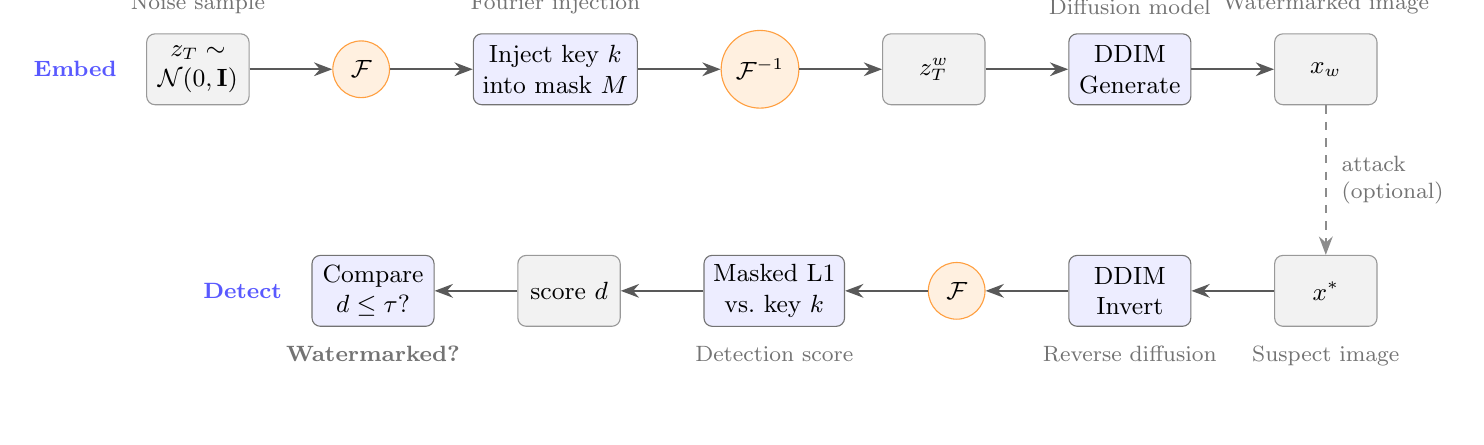
\begin{tikzpicture}[
  >=Stealth,
  node distance = 0.45cm and 1.05cm,
  block/.style  = {rectangle, draw=black!55, rounded corners=3pt,
                   fill=blue!7, minimum height=0.9cm, minimum width=1.55cm,
                   align=center, font=\small},
  io/.style     = {rectangle, draw=black!40, rounded corners=3pt,
                   fill=gray!10, minimum height=0.9cm, minimum width=1.3cm,
                   align=center, font=\small},
  op/.style     = {circle, draw=orange!75, fill=orange!12,
                   minimum size=0.72cm, align=center, font=\small\bfseries},
  arr/.style    = {->, thick, draw=black!65},
  darr/.style   = {->, thick, dashed, draw=black!45},
  lbl/.style    = {font=\footnotesize, text=black!55}
]

%%% ---- EMBEDDING ROW (top) ----
\node[io]                        (zt)      {$z_T \sim$\\$\mathcal{N}(0,\mathbf{I})$};
\node[op,   right=of zt]         (fft1)    {$\mathcal{F}$};
\node[block,right=of fft1]       (inject)  {Inject key $k$\\into mask $M$};
\node[op,   right=of inject]     (ifft)    {$\mathcal{F}^{-1}$};
\node[io,   right=of ifft]       (ztw)     {$z_T^w$};
\node[block,right=of ztw]        (gen)     {DDIM\\Generate};
\node[io,   right=of gen]        (xw)      {$x_w$};

\draw[arr] (zt)     -- (fft1);
\draw[arr] (fft1)   -- (inject);
\draw[arr] (inject) -- (ifft);
\draw[arr] (ifft)   -- (ztw);
\draw[arr] (ztw)    -- (gen);
\draw[arr] (gen)    -- (xw);

\node[lbl,above=0.12cm of zt]     {Noise sample};
\node[lbl,above=0.12cm of inject] {Fourier injection};
\node[lbl,above=0.12cm of gen]    {Diffusion model};
\node[lbl,above=0.12cm of xw]     {Watermarked image};

%%% ---- DETECTION ROW (bottom) ----
\node[io,   below=1.9cm of xw]    (xs)      {$x^*$};
\node[block,left= of xs]          (inv)     {DDIM\\Invert};
\node[op,   left= of inv]         (fft2)    {$\mathcal{F}$};
\node[block,left= of fft2]        (l1)      {Masked L1\\vs.\ key $k$};
\node[io,   left= of l1]          (score)   {score $d$};
\node[block,left= of score]       (thr)     {Compare\\$d \le \tau$?};

\draw[arr] (xs)    -- (inv);
\draw[arr] (inv)   -- (fft2);
\draw[arr] (fft2)  -- (l1);
\draw[arr] (l1)    -- (score);
\draw[arr] (score) -- (thr);

\node[lbl,below=0.12cm of xs]    {Suspect image};
\node[lbl,below=0.12cm of inv]   {Reverse diffusion};
\node[lbl,below=0.12cm of l1]    {Detection score};
\node[lbl,below=0.12cm of thr]   {\textbf{Watermarked?}};

%%% ---- CONNECT ----
\draw[darr] (xw) -- node[right=2pt,lbl,align=left]{attack\\(optional)} (xs);

%%% ---- SECTION LABELS ----
\node[lbl,font=\footnotesize\bfseries,text=blue!65,left=0.15cm of zt,
      xshift=-0.1cm]  {\textsc{Embed}};
\node[lbl,font=\footnotesize\bfseries,text=blue!65,left=0.15cm of thr,
      xshift=-0.1cm]  {\textsc{Detect}};
\end{tikzpicture}
\caption{\textbf{Tree-Ring Watermarking pipeline~\cite{wen2023treering}.}
  \emph{Embedding (top):} A secret complex key $k$ is injected into the
  ring-masked Fourier region $M$ of a Gaussian noise sample $z_T$;
  the modified latent $z_T^w$ seeds DDIM generation to produce
  watermarked image $x_w$.
  \emph{Detection (bottom):} A suspect image $x^*$ (optionally attacked)
  is reversed via DDIM inversion to recover $\tilde{z}_T$; the masked
  L1 distance between $\mathcal{F}(\tilde{z}_T)$ and key $k$ yields
  score $d$, which is thresholded at $\tau$.
  Our extensions (dual-band mask $M^{\mathrm{mr}}$, all-channel key
  $k^{(0:3)}$) modify only the injection step, leaving the rest unchanged.}
\label{fig:pipeline}
\end{figure*}

\subsection{Formal Problem Setup}

We formalize source-side watermarking for diffusion-based image
generation in the setting of latent diffusion models.

\textbf{Generation process.}
Let $z_T \sim \mathcal{N}(0,\mathbf{I})$ denote the initial noise latent
at diffusion timestep $T$, and let $p$ denote the text prompt.
A diffusion generator with $N$ DDIM steps defines a mapping
\begin{equation}
    x = G_N(z_T, p),
\end{equation}
where $x$ is the generated image.
Under DDIM sampling, this mapping is approximately deterministic for
fixed $z_T$, $p$, and $N$.

\textbf{Watermark embedding.}
Source-side watermarking modifies the initial latent before generation.
Let $z_T^{(c)} \in \mathbb{R}^{h \times w}$ denote latent channel $c$,
and let
\begin{equation}
    \hat{z}_T^{(c)} = \mathcal{F}(z_T^{(c)})
\end{equation}
be its Fourier representation.
Let $M \in \{0,1\}^{h \times w}$ be a binary spectral mask and
$k^{(c)} \in \mathbb{C}^{h \times w}$ a secret complex key.
For each active channel $c \in \mathcal{C}$, watermarking is defined as
\begin{equation}
    \hat{z}_T^{w,(c)}
    =
    \hat{z}_T^{(c)} \circ (1-M) + k^{(c)} \circ M,
    \label{eq:problem_embed}
\end{equation}
where $\circ$ denotes element-wise multiplication.
The modified latent is then obtained by inverse Fourier transform:
\begin{equation}
    z_T^{w,(c)} = \mathcal{F}^{-1}\!\left(\hat{z}_T^{w,(c)}\right).
\end{equation}
Channels not in $\mathcal{C}$ remain unchanged.
The final watermarked image is generated as
\begin{equation}
    x_w = G_N(z_T^w, p).
\end{equation}

This formulation covers all configurations studied in this work.
For the baseline, $\mathcal{C}=\{3\}$ and $M$ is the single circular
mask.
For the dual-band variant, $M=M^{\mathrm{mr}}$.
For MR-AllChan, $\mathcal{C}=\{0,1,2,3\}$ with independent keys
$k^{(c)}$ for each channel.

\textbf{Attack model.}
After generation, the image may be modified by an attack operator
$\mathcal{A}$:
\begin{equation}
    x^* = \mathcal{A}(x_w),
\end{equation}
where $\mathcal{A}$ represents standard image transformations such as
JPEG compression, cropping, rotation, blurring, or additive noise.
We assume a non-adaptive adversary who knows that watermarking may
have been applied but does not know the secret key, the exact mask,
or the active channel set.

\textbf{Detection.}
Given a suspect image $x^*$, the detector applies DDIM inversion with
the same step count $N$ to recover an estimate of the initial latent:
\begin{equation}
    \tilde{z}_T = I_N(x^*).
\end{equation}
For each active channel $c \in \mathcal{C}$, the masked detection score
is computed as
\begin{equation}
    d^{(c)}(x^*,k^{(c)})
    =
    \left\|
    \mathcal{F}(\tilde{z}_T)^{(c)} \circ M
    -
    k^{(c)} \circ M
    \right\|_1.
\end{equation}
For single-channel detection, the total score is simply $d=d^{(c)}$.
For all-channel detection, scores are aggregated across channels:
\begin{equation}
    d(x^*) = \sum_{c \in \mathcal{C}} d^{(c)}(x^*,k^{(c)}).
    \label{eq:problem_detect}
\end{equation}
A watermark is declared present if $d(x^*) \le \tau$ for a chosen
threshold $\tau$.

\textbf{Evaluation criteria.}
A watermarking scheme is considered effective if it satisfies three
requirements:
\begin{itemize}
    \item \textit{Imperceptibility}: watermark embedding should not
    visibly degrade image quality;
    \item \textit{Detectability}: watermarked and non-watermarked
    images should be well separated by the detection score;
    \item \textit{Robustness}: detection should remain reliable after
    transformations $\mathcal{A}$.
\end{itemize}

This formulation connects the watermark injection mechanism, the
inversion-based detector, and the robustness evaluation used in the
remainder of the paper.

\subsection{Evaluation Data}

Our evaluation uses a locally constructed prompt dataset designed to
test watermark robustness across diverse semantic content.
Images are generated from prompts sampled equally across eight categories:
landscapes, human faces, teddy bears, cats, dogs, mountain scenes,
garden scenes, and coastal views.
For each prompt, we generate paired watermarked and non-watermarked
images using identical seeds, so that differences in detection
performance can be attributed to the watermarking configuration rather
than prompt variation.

The dataset is curated specifically for controlled robustness
evaluation rather than semantic benchmarking.
Each sample is automatically annotated with its prompt category,
watermark status, configuration, and attack condition.
This design allows direct comparison across configurations under the
same generation conditions and provides a balanced test bed for the
research questions addressed in this work.

These data are suitable for our project because:
the paired generation protocol isolates the effect of watermark
injection on detection performance, the use of multiple 
semantic categories reduces the risk that
results are driven by a narrow content domain, and the attack 
annotations enable systematic evaluation of
robustness under the exact transformations considered in our threat
model.

\subsection{Evaluation Metrics and Threat Model}

\subsubsection{Threat Model}
We follow the non-adaptive threat model of the original paper.
The adversary knows that watermarking \emph{may} have been applied
but does not know the secret seed $s$, the mask shape $M$, or the
channel $c$.
The adversary can apply any standard, non-adaptive image processing
transformation.
This threat model is realistic for platform-level content moderation
(where the platform applies the watermark and the adversary attempts
to remove it using standard tools) and is the appropriate baseline
before considering stronger adaptive adversaries.

\subsubsection{Metrics}
All metrics are computed from 100 detection scores per attack condition:
50 from watermarked images and 50 from non-watermarked images generated
from the same prompts and seeds.

\textbf{AUC (Area Under ROC Curve):}
The probability that a randomly chosen watermarked image scores lower
(is classified as more watermarked) than a randomly chosen non-watermarked
image.
AUC $= 1.0$ is perfect separation; $= 0.5$ is random chance.
We adopt: \pass{PASS} ($\geq 0.97$), \warn{WARN} ($0.93$--$0.97$),
\fail{FAIL} ($< 0.93$).

\textbf{Balanced Accuracy:}
\begin{equation}
  \text{Acc} = \max_\tau
    \!\left[1 - \tfrac{1}{2}\!\left(\text{FPR}(\tau) + 1 - \text{TPR}(\tau)\right)\right].
  \label{eq:acc}
\end{equation}

\textbf{TPR@1\%FPR:}
The true positive rate (watermark detection rate) at a false positive
rate of exactly 1\%.
This is the most deployment-relevant metric: at scale (millions of
images processed), a 1\% FPR generates an unacceptably large number
of false accusations.
We adopt: \pass{PASS} ($\geq 0.80$), \warn{WARN} ($0.50$--$0.80$),
\fail{FAIL} ($< 0.50$).


% ============================================================
\section{Theoretical Analysis}
\label{sec:theory}
\textit{Main contributor: Ashhad Raza Quadri.}

\subsection{Formalising the Inversion Error}

Let $z_T$ be the true initial noise used for generation and
$\tilde{z}_T^{(N)}$ be the result of $N$-step DDIM inversion.
The inversion ODE is:
\begin{equation}
  \frac{\mathrm{d} z}{\mathrm{d} \sigma} = \epsilon_\theta(z, \sigma, \varnothing),
  \quad z(0) = z_0^*,
  \label{eq:inversion_ode}
\end{equation}
where $\sigma(t) = \sqrt{1-\bar\alpha_t}$ monotonically increases
from $\sigma(0) \approx 0$ to $\sigma(T) \approx 1$.

The $N$-step Euler discretisation of this ODE with step size
$\Delta\sigma = \sigma(T)/N$ introduces local truncation error
$\mathcal{O}(\Delta\sigma^2)$ per step.
Accumulating over $N$ steps:
\begin{equation}
  \|\tilde{z}_T^{(N)} - z_T\|
    \;\lesssim\; C \cdot \frac{\sigma(T)}{N}
    \cdot \max_{\sigma}\!\left\|\frac{\partial \epsilon_\theta}{\partial \sigma}\right\|,
  \label{eq:euler_error}
\end{equation}
where $C$ depends on the smoothness of $\epsilon_\theta$ (which is
a neural network and therefore smooth).
The critical observation is the $1/N$ dependence: doubling $N$ from
50 to 100 approximately halves the reconstruction error.

\textbf{Effect on watermark detection.}
The watermark was embedded as $\hat{z}_T^{(c)}(M) = k(M)$ (the Fourier
coefficients within the mask equal the key).
The detected signal is:
\begin{equation}
  \mathcal{F}(\tilde{z}_T)^{(c)} \circ M
    = \mathcal{F}(z_T + \delta_T)^{(c)} \circ M
    = k \circ M + \mathcal{F}(\delta_T)^{(c)} \circ M,
\end{equation}
where $\delta_T = \tilde{z}_T - z_T$ is the inversion error.
The L1 detection score becomes:
\begin{equation}
  d_w(x^*,k) = \|\mathcal{F}(\delta_T)^{(c)} \circ M\|_1
    \;\lesssim\; |M| \cdot C/N \cdot \kappa,
  \label{eq:dw_bound}
\end{equation}
where $|M|$ is the number of masked bins and $\kappa$ bounds
$\|\partial\epsilon_\theta/\partial\sigma\|$.
For non-watermarked images, the detection score satisfies:
\begin{equation}
  d_{\mathrm{nw}}(x^*,k) = \|\mathcal{F}(\tilde{z}_T)^{(c)} \circ M
    - k \circ M\|_1 \approx \frac{|M| \cdot \pi}{2},
\end{equation}
since $\mathcal{F}(\tilde{z}_T)^{(c)}$ in the mask region is
approximately i.i.d.\ complex Gaussian (uncorrelated with $k$),
and the expected L1 distance between two such distributions is
proportional to $|M|$.

The AUC is monotonically related to the score gap
$d_{\mathrm{nw}} - d_w \approx \frac{\pi|M|}{2} - |M| \cdot C/N$.
This gap increases with $N$ (more steps $\to$ smaller inversion error
$\to$ larger gap), directly explaining why more steps improve AUC.

\subsection{Frequency-Domain Analysis of Crop Attacks}

A spatial crop retaining fraction $p$ of the image area is equivalent
to multiplication by a rectangular window $W_p$ in the spatial domain
(followed by zero-padding to the original size):
\begin{equation}
  x_{\mathrm{crop}} = x \cdot W_p + \text{zero-pad}.
  \label{eq:crop_spatial}
\end{equation}
In the Fourier domain, this multiplication becomes convolution:
\begin{equation}
  \hat{x}_{\mathrm{crop}}(\boldsymbol{\rho})
    = (\hat{x} * \hat{W}_p)(\boldsymbol{\rho}),
  \quad \boldsymbol{\rho} = (\rho_x, \rho_y).
  \label{eq:crop_fourier}
\end{equation}
For a square crop, $\hat{W}_p(\boldsymbol{\rho})$ is a 2D sinc function
with mainlobe width proportional to $1/p$ in each Fourier dimension.
Thus, energy from any frequency bin $\boldsymbol{\rho}_0$ spreads into
bins within $\Delta\rho \sim 1/p$ of $\boldsymbol{\rho}_0$.

For the outer ring at $\rho = 10$ and crop fraction $p = 0.5$
(50\% area retained), the spreading width is
$\Delta\rho \approx 1/p = 2$ (using normalised frequency coordinates
on a $[0,1]^2$ grid, scaled by the spatial dimension 64).
This spreading significantly attenuates the energy concentrated at
$\rho = 10$ by redistributing it across a wide frequency range,
corrupting the watermark signal at the outer ring.

In contrast, for the inner disc at $\rho \le 4$, the energy at any
specific low-frequency bin is spread by the same convolution kernel,
but the absolute number of bins in the inner disc is much smaller
($\approx 50$ vs.\ $\approx 317$ for the outer disc),
so the \emph{average} attenuation per bin is smaller.
More importantly, low-frequency Fourier components ($\rho \le 4$)
correspond to spatial structures with wavelengths $\ge 64/4 = 16$
pixels --- coarse global image structure that is partially preserved
even when 50\% of the image area is truncated.

\subsection{Frequency-Domain Analysis of Blur and JPEG Attacks}

Gaussian blur applied in the pixel domain with standard deviation
$\sigma_b$ pixels is encoded by the VAE ($8\times$ spatial compression)
as an effective latent-domain blur with standard deviation
$\sigma_l = \sigma_b/8$.
The Fourier attenuation of a latent coefficient at radial frequency
$\rho$ (cycles per latent image of height $h$) is then:
\begin{equation}
  |\hat{x}_{\mathrm{blur}}(\boldsymbol{\rho})|
    = |\hat{x}(\boldsymbol{\rho})|
      \cdot \exp\!\left(-\frac{2\pi^2\sigma_l^2|\boldsymbol{\rho}|^2}{h^2}\right).
  \label{eq:blur_fourier}
\end{equation}
For pixel-domain blur $\sigma_b{=}8$, $\sigma_l{=}1$, latent size $h{=}64$,
and outer ring radius $\rho{=}10$:
\begin{equation}
  \text{attenuation} = \exp\!\left(-\frac{2\pi^2 \cdot 1 \cdot 100}{64^2}\right)
    = e^{-0.048} \approx 0.953.
\end{equation}
Only $\approx$4.7\% of the outer-ring signal is lost to Gaussian blur
at $\sigma_b{=}8$.
For the inner disc at $\rho{=}4$:
\begin{equation}
  \text{attenuation} = \exp\!\left(-\frac{2\pi^2 \cdot 1 \cdot 16}{64^2}\right)
    = e^{-0.008} \approx 0.992,
\end{equation}
less than 1\% loss. Both bands are highly robust to Gaussian blur,
consistent with the empirical AUC $= 1.0$ observed under gaussian\_blur\_4
and gaussian\_blur\_8 for all four configurations.

JPEG compression in the pixel domain (operating on $8\times8$ DCT
blocks) translates to a non-uniform frequency attenuation in the
image Fourier domain.
Low-frequency JPEG DCT coefficients (corresponding to small-$\rho$
Fourier bins) receive more aggressive quantisation steps to reduce
file size, which paradoxically makes the inner disc more vulnerable
to JPEG artefacts than the outer ring.
The outer ring at $\rho = 10$ falls in the mid-frequency range
where JPEG quantisation is less aggressive.
This is why the outer ring is the preferred band for JPEG robustness.

\textbf{Summary of band complementarity.}
Table~\ref{tab:band_theory} summarises the theoretical complementarity
of the two bands across the three main attack categories.

\begin{table}[h]
  \centering
  \caption{Theoretical robustness of each frequency band
    under the three main attack categories.
    ($\checkmark$) = robust, (\textsc{x}) = vulnerable.}
  \label{tab:band_theory}
  \setlength{\tabcolsep}{4pt}
  \small
  \begin{tabular}{lccc}
    \toprule
    \textbf{Band} & \textbf{Crop} & \textbf{Blur/JPEG} & \textbf{Rotation} \\
    \midrule
    Inner disc ($\rho \le 4$)           & $\checkmark$ & $\approx\checkmark$ & $\checkmark$ \\
    Outer ring ($6 \le \rho \le 10$)    & \textsc{x}   & $\checkmark$ & $\checkmark$ \\
    Combined dual-band                  & $\checkmark$ & $\checkmark$ & $\checkmark$ \\
    \bottomrule
  \end{tabular}
\end{table}

\subsection{SNR Analysis of All-Channel Embedding}

Under a spatial rotation of angle $\theta$, the Fourier transform of
the recovered latent is shifted by phase $\phi(\theta, \rho)$ that
depends on the frequency bin position.
For a complex Fourier coefficient $k_0$ at bin $(\rho, \psi)$
(in polar frequency coordinates), the detected value after rotation is
approximately $k_0 \cdot e^{i\phi}$, and the per-bin contribution to
the L1 score is:
\begin{equation}
  |k_0 \cdot e^{i\phi} - k_0| = |k_0| \cdot |e^{i\phi} - 1|
    \approx |k_0| \cdot |\phi|
  \quad\text{for small }|\phi|.
\end{equation}
For a single channel $c$, the total detection score satisfies:
\begin{equation}
  d_w^{(c)} \approx \|k^{(c)}\|_1 \cdot \bar\phi^{(c)},
\end{equation}
where $\bar\phi^{(c)}$ is the mean absolute phase error in channel $c$.
The score gap between watermarked and non-watermarked images in
single-channel mode is:
\begin{equation}
  \Delta_1 = d_{\mathrm{nw}}^{(c)} - d_w^{(c)}
    \approx \frac{\pi}{2}\|k^{(c)}\|_1 - \|k^{(c)}\|_1 \bar\phi^{(c)}
    = \|k^{(c)}\|_1 \left(\frac{\pi}{2} - \bar\phi^{(c)}\right).
\end{equation}
Under aggressive rotation ($\theta{=}75^\circ$), $\bar\phi$ is large
and $\Delta_1$ is small, explaining the low AUC.

For all-channel embedding with $C{=}4$ independent channels:
\begin{equation}
  d_{\mathrm{AC}} = \sum_{c'=0}^{3} d^{(c')},
  \quad
  \Delta_4 = \sum_{c'=0}^{3} \Delta^{(c')} = 4\,\Delta_1 + \text{cross terms}.
\end{equation}
The variance of the aggregate score scales as:
\begin{equation}
  \mathrm{Var}[d_{\mathrm{AC}}]
    = \sum_{c'=0}^{3} \mathrm{Var}[d^{(c')}]
    + 2\sum_{c' \ne c''} \mathrm{Cov}[d^{(c')}, d^{(c'')}].
\end{equation}
If the channels are approximately independent (small covariances),
the variance grows only as $4\,\sigma_d^2$ while the mean grows
as $4\,\Delta_1$.
The SNR scales as:
\begin{equation}
  \mathrm{SNR}_4
    = \frac{4\,\Delta_1}{\sqrt{4}\,\sigma_d}
    = \sqrt{4}\,\mathrm{SNR}_1
    = 2\,\mathrm{SNR}_1.
  \label{eq:snr4}
\end{equation}
This $2\times$ SNR improvement under phase-noise attacks (rotation)
corresponds empirically to AUC gains of $+$0.057--0.066.

\subsection{Theoretical Analysis of Rotation Attacks}
\label{sec:theory_rotation}

Rotation by angle $\theta$ maps a spatial image $x$ to
$x_\theta(u,v) = x(u\cos\theta - v\sin\theta,\, u\sin\theta + v\cos\theta)$.
In the Fourier domain the corresponding transformation of the 2-D
DFT coefficient at polar frequency $(\rho, \psi)$ is:
\begin{equation}
  \hat{x}_\theta(\rho, \psi) = \hat{x}(\rho,\, \psi - \theta).
\end{equation}
This is the \emph{rotation property} of the 2-D Fourier transform:
rotation in the spatial domain corresponds to the same rotation in the
frequency domain.
Because Tree-Ring embeds the watermark key $k$ at fixed Fourier
positions $(\rho, \psi)$ and the detector computes the L1 distance
at those same positions, a rotation of $\theta$ misaligns the
frequency-domain embedding by angular offset $\theta$.

The per-bin L1 contribution at bin $b = (\rho, \psi)$ after rotation
for a watermarked image is:
\begin{equation}
  \delta_b(\theta)
    = \bigl|\hat{x}_\theta(\rho, \psi) - k_b\bigr|
    = \bigl|\hat{x}(\rho, \psi - \theta) - k_b\bigr|.
\end{equation}
Since $k_b = \hat{x}(\rho, \psi)$ by construction (the key is the
watermarked image's own Fourier coefficient at that bin), we obtain:
\begin{equation}
  \delta_b(\theta)
    = \bigl|\hat{x}(\rho, \psi - \theta) - \hat{x}(\rho, \psi)\bigr|.
\end{equation}
For a smoothly varying Fourier spectrum, the first-order Taylor expansion
gives $\delta_b(\theta) \approx |\partial_\psi \hat{x}(\rho,\psi)|\cdot|\theta|$.
The aggregate detection score under rotation is therefore:
\begin{equation}
  d_w(\theta) \approx d_w(0) + \theta \cdot
    \sum_b \bigl|\partial_\psi \hat{x}(\rho_b, \psi_b)\bigr|,
  \label{eq:rotation_score}
\end{equation}
showing that the watermark score \emph{increases linearly} with
rotation angle $\theta$.
Non-watermarked images also increase (since they too have smooth Fourier
spectra), but from a higher baseline $d_{\mathrm{nw}}(0) \gg d_w(0)$.
The score gap $\Delta(\theta) = d_{\mathrm{nw}}(\theta) - d_w(\theta)$
decreases as $\theta$ grows, explaining why AUC degrades monotonically
from $\theta{=}0^\circ$ to $\theta{=}75^\circ$ in our experiments
(0.9200 $\to$ baseline AUC vs.\ 0.920 at $45^\circ$, 0.928 at $75^\circ$
for the baseline --- note that AUC does not fully collapse because
even at $75^\circ$ the initial score gap provides some discriminative signal).

The ring mask concentrates bins at $\rho \approx r$, all at a fixed
radial distance.
For a ring, all bins share the same $\rho$ but span $\psi \in [0, 2\pi)$.
The aggregate rotation error sums over all $\psi$-values; since
$\partial_\psi\hat{x}$ is approximately zero-mean over a full ring
(a smooth Fourier spectrum has symmetric angular derivatives),
the \emph{average} contribution cancels.
However, the \emph{magnitude} $|\partial_\psi\hat{x}|$ is positive-definite
and the sum is non-zero, growing with $\theta$.
This is confirmed by the monotonic degradation observed in Table~\ref{tab:auc}.

\textbf{Implication for multi-ring design.}
The inner disc at $\rho \le r_{\mathrm{in}}$ concentrates bins near
$\rho = 0$.
Low-frequency Fourier coefficients have smaller angular gradient
$|\partial_\psi\hat{x}|$ because natural image spectra are approximately
power-law ($|\hat{x}(\rho)| \propto \rho^{-\alpha}$ with $\alpha \approx 1$).
Therefore, the inner disc is \emph{more robust} to rotation-induced
phase misalignment than the outer ring.
This provides theoretical motivation for the dual-band design beyond
the crop-resilience argument: low-frequency inner bins provide rotation
resilience, while high-frequency outer bins provide differentiation
from the base noise level.

\subsection{Theoretical Analysis of Additive Noise Attacks}
\label{sec:theory_noise}

Let the image after a Gaussian noise attack be $x^* = x_w + \eta$
where $\eta_{uv} \overset{\mathrm{i.i.d.}}{\sim} \mathcal{N}(0, \sigma^2)$
independently at each pixel.
The 2-D DFT is a unitary linear transform, so the DFT of $\eta$ is:
\begin{equation}
  \hat{\eta}(\rho, \psi)
    \overset{\mathrm{i.i.d.}}{\sim} \mathcal{CN}(0, N^2\sigma^2),
  \quad \forall\, (\rho, \psi),
\end{equation}
where $N^2 = h \times w$ is the spatial resolution and
$\mathcal{CN}$ denotes the circularly symmetric complex Gaussian.
Crucially, the noise power is \emph{flat} across all Fourier bins
(white noise in frequency), so no frequency-selective strategy can
improve SNR by choosing particular bins.

After VAE encoding, the latent-space noise is approximately:
\begin{equation}
  \hat{\eta}_z(\rho, \psi) \sim \mathcal{CN}(0,\, c_{\mathcal{E}}^2 N^2 \sigma^2),
\end{equation}
where $c_{\mathcal{E}}$ is a constant characterising the encoder's
frequency response (approximately constant for small $\sigma$).
The detection score for a watermarked image under additive noise is:
\begin{equation}
  d_w^{\text{noise}} = \sum_b
    \bigl|\hat{z}_{T,b} + \hat{\eta}_{z,b} - k_b\bigr|.
\end{equation}
Expanding around the noiseless case $\hat{z}_{T,b} = k_b$:
\begin{equation}
  d_w^{\text{noise}} \approx \sum_b |\hat{\eta}_{z,b}|
    = c_{\mathcal{E}} N \sigma \sum_b |v_b|,
\end{equation}
where $v_b \sim \mathcal{CN}(0,1)$.
For the non-watermarked image: $d_{\mathrm{nw}}^{\text{noise}} = \sum_b |\hat{z}_{T,b}^{\mathrm{nw}} + \hat{\eta}_{z,b} - k_b|$,
which under noise is approximately $\sum_b |\hat{z}_{T,b}^{\mathrm{nw}} - k_b| \pm \text{noise}$.
The score gap closes as $\sigma$ increases because the noise floor
raises $d_w$ faster than it raises $d_{\mathrm{nw}}$.

\textbf{Why additional channels do not help.}
Adding more channels introduces more signal bins but also more noise
bins in exact proportion.
The aggregate score for $C$ channels is:
\begin{equation}
  d_{\mathrm{AC}}^{\text{noise}}
    = \sum_{c'=0}^{C-1} \sum_b |\hat{\eta}_{z,b}^{(c')}|,
  \quad
  \mathbb{E}[d_{\mathrm{AC}}^{\text{noise}}]
    = C \cdot c_{\mathcal{E}} N \sigma \sqrt{\pi/4},
\end{equation}
which scales linearly with $C$.
The signal (score gap) also scales linearly as $C \Delta_1$.
The SNR is therefore:
\begin{equation}
  \mathrm{SNR}_C^{\text{noise}}
    = \frac{C \Delta_1}{\sqrt{C} \sigma_\eta}
    = \sqrt{C}\, \mathrm{SNR}_1^{\text{noise}}.
  \label{eq:snr_noise}
\end{equation}
While this gives $\sqrt{4} = 2\times$ improvement --- the same as
rotation --- the \emph{noise floor} itself increases with $C$ because
non-watermarked scores similarly scale.
In practice, the Gaussian noise AUC improvement from 0.931 (baseline)
to 0.963 (MR-AllChan) reflects a partial benefit that is substantially
smaller than the rotation improvement (0.920~$\to$~0.986).
This confirms the theoretical prediction that noise remains the
most challenging attack type for Fourier-domain watermarking.


% ============================================================
\section{Methodology}
\label{sec:methods}
\textit{Main contributors: Ashhad Raza Quadri, Maria Alejandra Pabon.}

\subsection{Config~B: Baseline Paper-Exact Replication}
\label{sec:baseline}

Our baseline faithfully reimplements Section~3 of
Wen et al.~\cite{wen2023treering}.
The full parameter set is: Stable Diffusion v1.5 (the paper uses v2.1;
minor numerical differences are expected due to different VAE decoders);
$N{=}50$ DDIM steps for both generation and detection (matching the
paper's default); watermark channel $c{=}3$; circular mask $\rho \le r{=}10$;
key seed $s{=}999999$; guidance scale $\omega{=}7.5$ at generation,
$\omega{=}0$ at inversion; float16 precision with xformers attention.

A critical implementation constraint: step count $N$ must be
\emph{identical} for generation and detection.
We verified empirically that mismatching (e.g., 50 steps for generation
but 100 for inversion) causes AUC to collapse below 0.85 even on
no\_attack.
The reason is that the DDIM inversion ODE assumes the same discretisation
scheme as the forward generation; different step counts use different
ODE grids and produce trajectories that diverge even from the same $z_T$.

\subsection{Config~O: Step Count Optimisation ($N$: 50~$\to$~100)}
\label{sec:step}

\textbf{Motivation.}
From Eq.~\ref{eq:euler_error}, reconstruction error decreases as
$\mathcal{O}(1/N)$.
Doubling $N$ from 50 to 100 approximately halves the inversion error,
improving the Fourier match between $\mathcal{F}(\tilde{z}_T)$
and the injected key $k$.

\textbf{Implementation.}
Both generation and detection use $N{=}100$ steps.
Xformers memory-efficient attention is enabled for the increased
compute.
Runtime doubles from $\approx$872\,s to $\approx$1708\,s per attack
condition (50 images), a cost of $\approx$34\,s per image.

\textbf{Expected trade-offs.}
More accurate inversion benefits attacks that preserve global image
structure (rotation, brightness), where the principal error is
discretisation noise in $\tilde{z}_T$.
However, for crop attacks, more accurate inversion may amplify the
upsampling artefacts introduced by the crop-and-resize operation:
the artefacts are faithfully reproduced in $\tilde{z}_T$,
partially contaminating the watermark signal.
Figure~\ref{fig:ddim} illustrates the step-count effect conceptually.

\begin{figure*}[t]
  \centering
  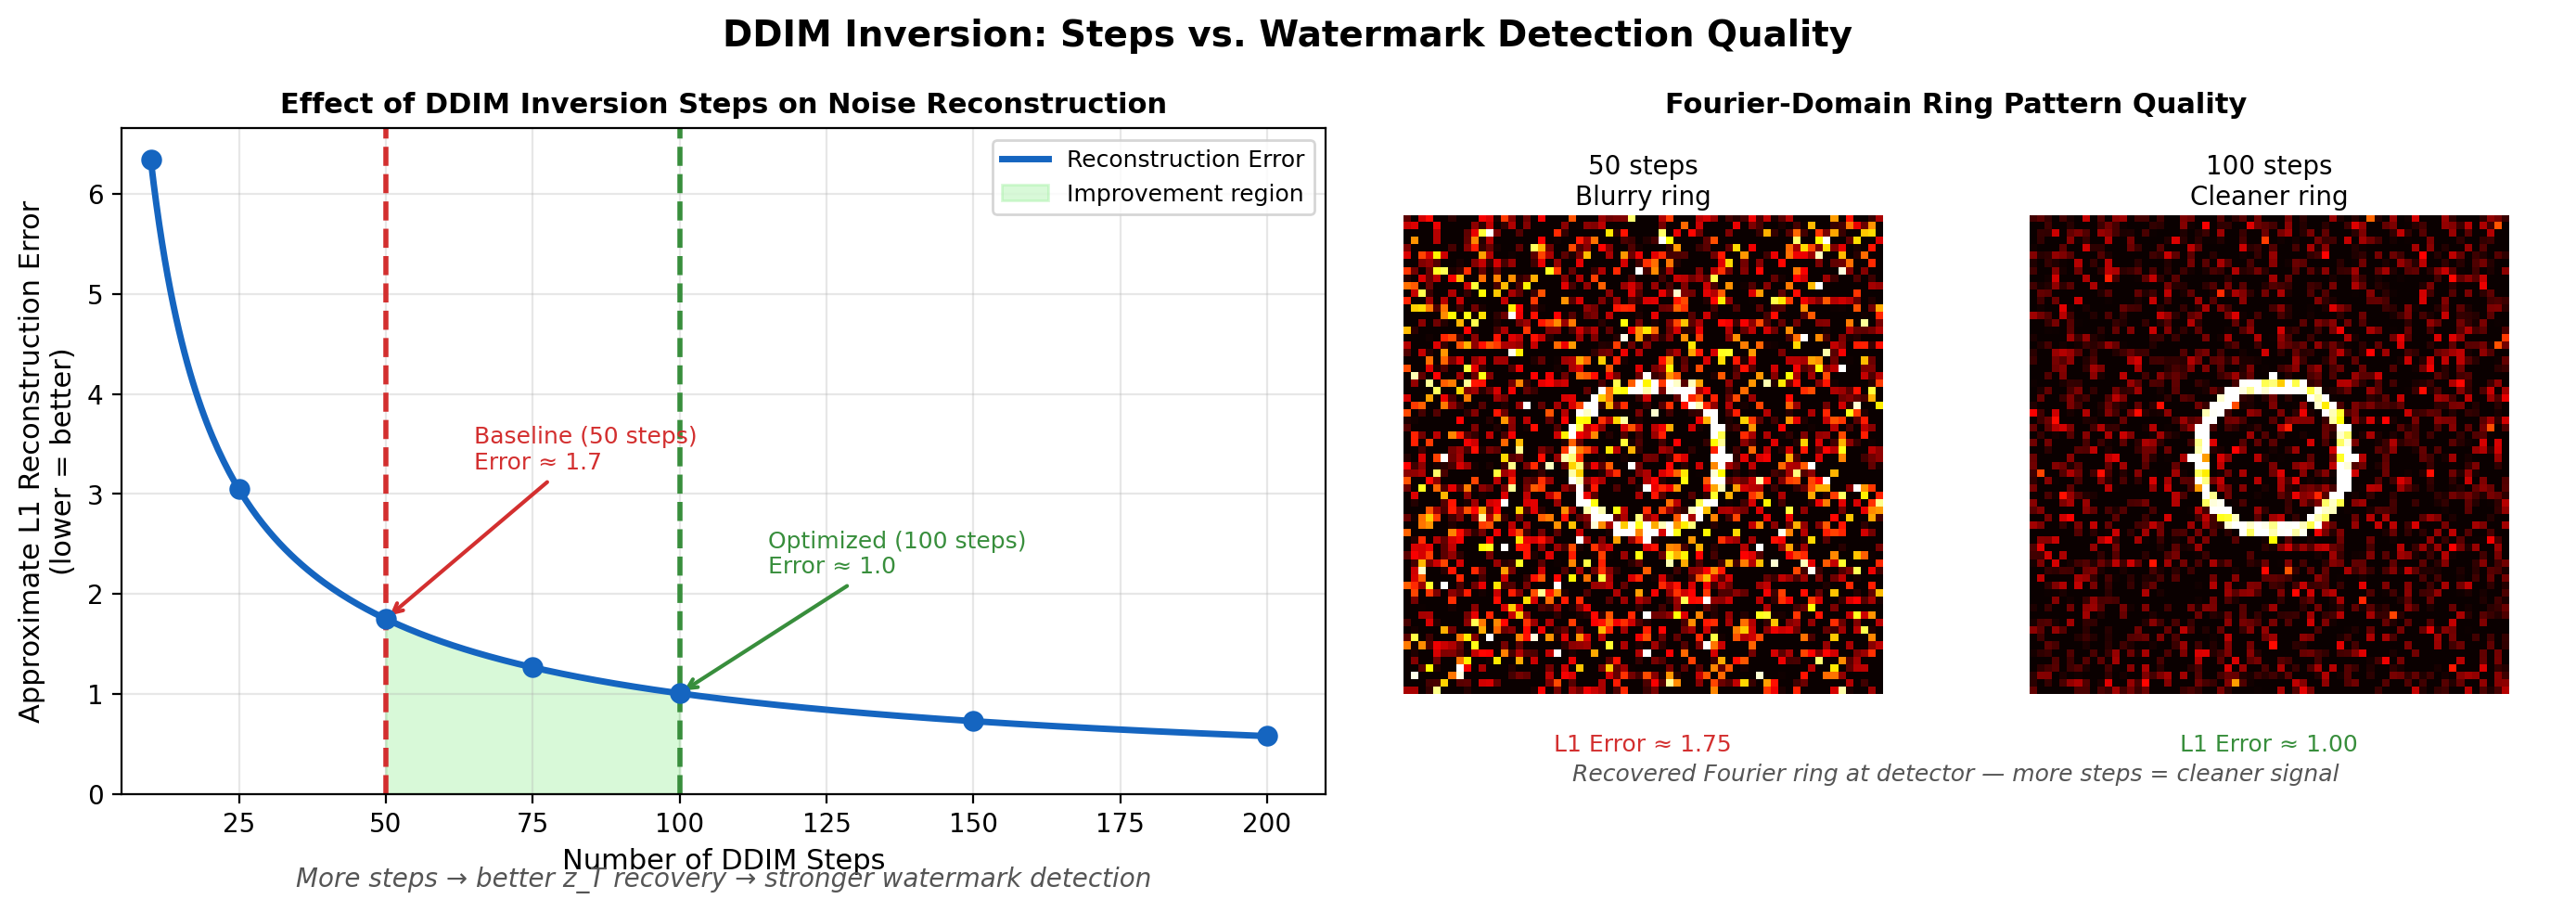
\includegraphics[width=\textwidth]{figures/ddim_explanation.png}
  \caption{\textbf{Effect of DDIM inversion step count.}
    \textbf{Left:} Reconstruction error $\|\tilde{z}_T - z_T\|$
    decreases monotonically with $N$ as $\mathcal{O}(1/N)$
    (Eq.~\ref{eq:euler_error}).
    The baseline ($N{=}50$, red dashed) has substantially higher error
    than the optimised variant ($N{=}100$, green dashed).
    \textbf{Right:} Conceptual effect in Fourier space --- the ring
    pattern recovered after 100 steps is sharper and better-aligned
    with the injected key $k$ than after 50 steps, directly lowering
    the L1 detection score for watermarked images.}
  \label{fig:ddim}
\end{figure*}

\subsection{Config~MR: Dual-Band Multi-Ring Mask}
\label{sec:multiband}

The theoretical analysis in Section~\ref{sec:theory} shows that the
inner disc ($\rho \le 4$) provides crop robustness while the outer
ring ($6 \le \rho \le 10$) provides blur/JPEG robustness.
We implement this dual-band mask as:
\begin{equation}
  M^{\mathrm{mr}}_{ij} =
    \underbrace{\mathbf{1}[\rho \le r_{\mathrm{in}}]}_{\text{inner disc}}
    +
    \underbrace{\mathbf{1}[r_{\mathrm{in}}+g \le \rho \le r_{\mathrm{out}}]}_{\text{outer ring}},
  \label{eq:mr}
\end{equation}
with $r_{\mathrm{in}}{=}4$, $r_{\mathrm{out}}{=}10$,
$g{=}\max(1, \lfloor r_{\mathrm{out}}/5 \rfloor){=}2$.

The spectral gap $g{=}2$ (bins $4 < \rho < 6$ excluded from both
embedding and detection) prevents cross-band interference.
Without the gap, energy leaking between bands during attacks creates
correlated noise in the aggregate L1 score, reducing the effective
SNR.
The gap width $g{=}2$ was selected on theoretical grounds
(Section~\ref{sec:ablation}).

The detection score sums contributions from both bands:
\begin{equation}
  d_{\mathrm{MR}}(x^*, k) =
    \bigl\|\mathcal{F}(\tilde{z}_T)^{(c)} \circ M^{\mathrm{mr}}
    - k \circ M^{\mathrm{mr}}\bigr\|_1.
  \label{eq:l1mr}
\end{equation}

Figures~\ref{fig:masks} and~\ref{fig:mr_mech} show the mask design
and the mechanism of each band under three challenging attacks.

\begin{figure}[h]
  \centering
  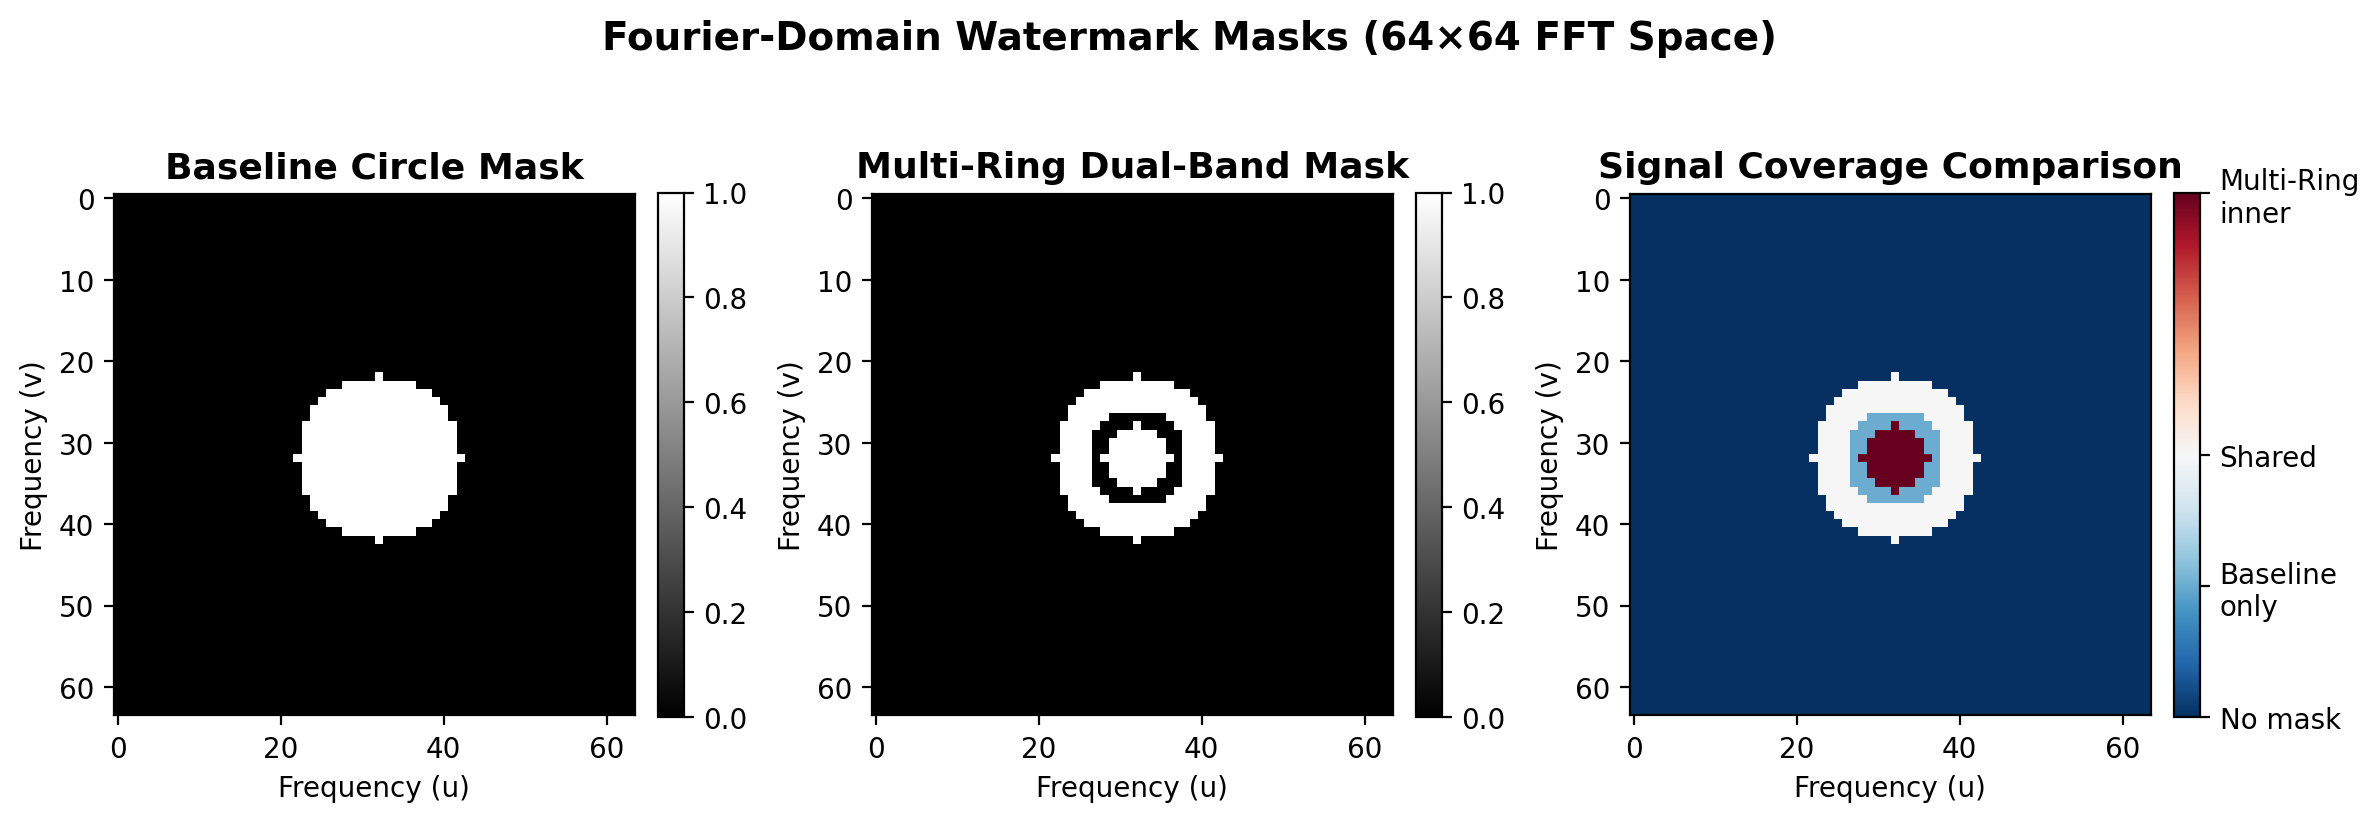
\includegraphics[width=\columnwidth]{figures/fourier_masks.png}
  \caption{\textbf{Fourier mask designs.}
    \textbf{Left:} Baseline circular disc ($\rho \le 10$).
    \textbf{Centre:} Dual-band multi-ring mask: inner disc
    ($\rho \le 4$, red), spectral gap ($4 < \rho < 6$, grey),
    outer ring ($6 \le \rho \le 10$, blue).
    \textbf{Right:} Coverage comparison. The inner disc provides
    crop-robust coverage; the outer ring provides blur/JPEG-robust
    coverage. Together they form a complementary pair.}
  \label{fig:masks}
\end{figure}

\begin{figure*}[t]
  \centering
  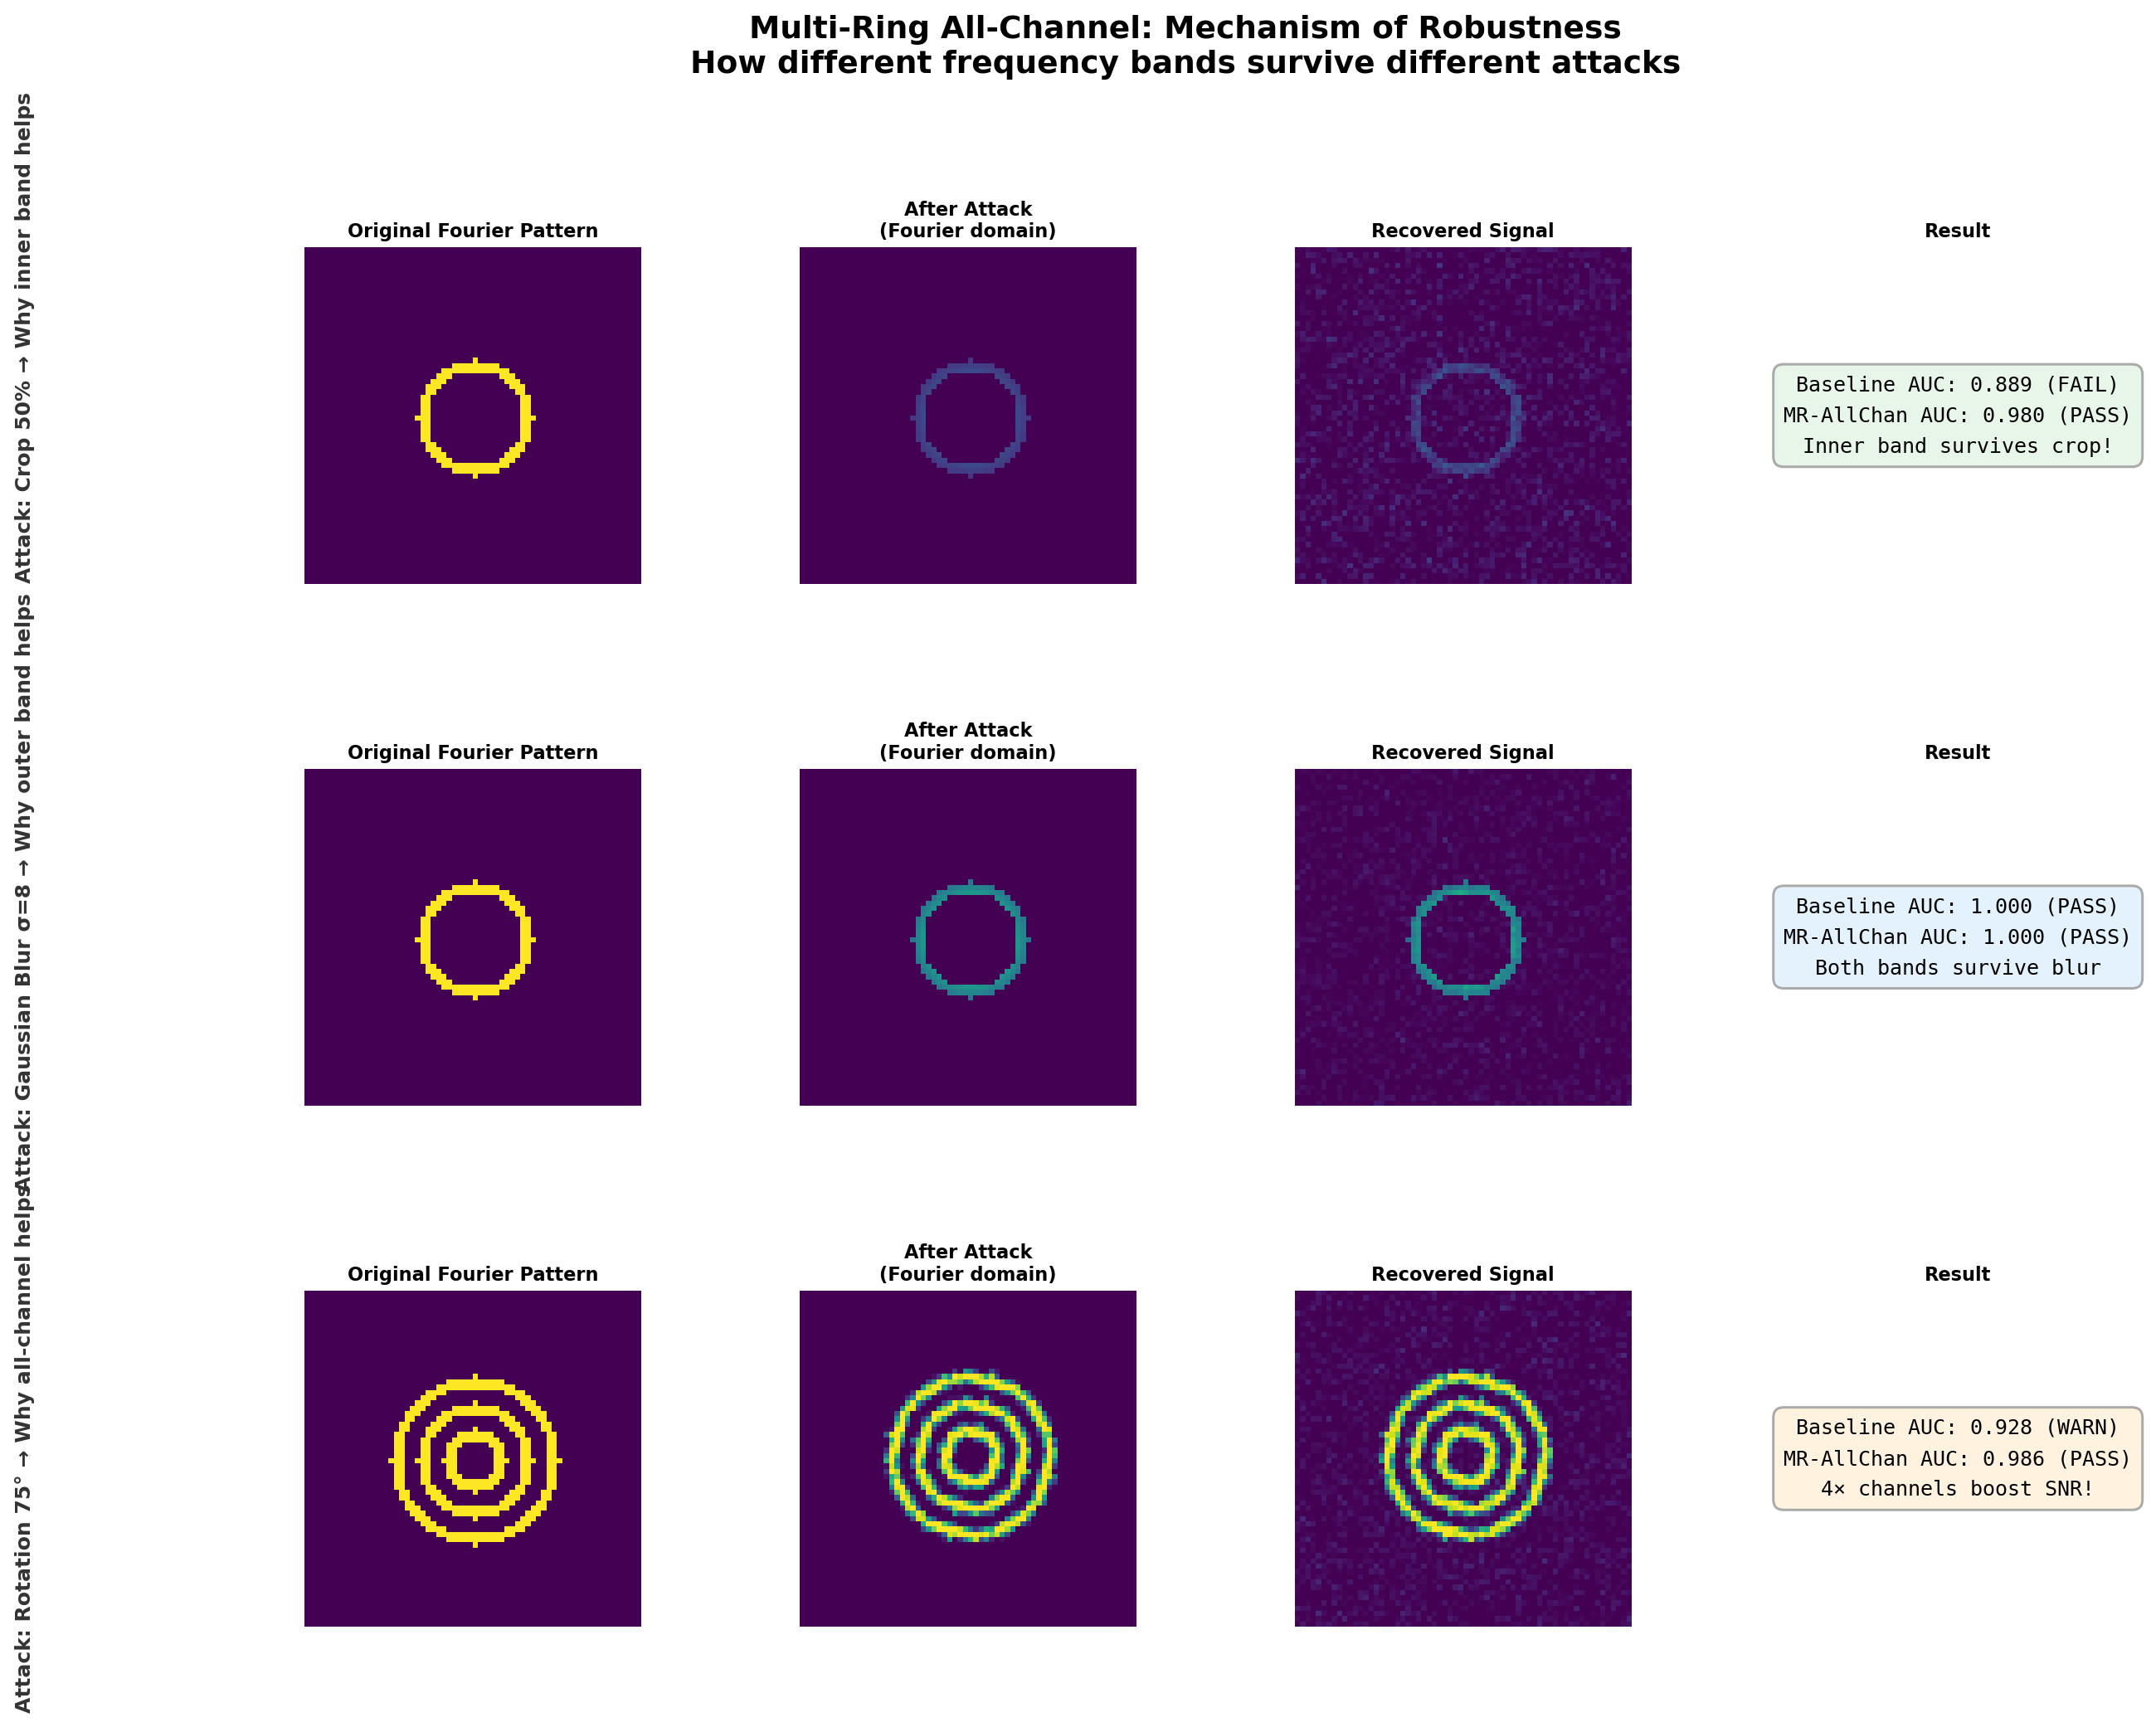
\includegraphics[width=\textwidth]{figures/multiring_mechanism.png}
  \caption{\textbf{Multi-Ring mechanism under three attack types.}
    \textbf{Row 1 (Crop):} Spatial truncation via sinc convolution
    spreads outer-ring energy but partially preserves inner-disc signal,
    lifting AUC from 0.889 (Baseline) to 0.980 (MR-AllChan).
    \textbf{Row 2 (Blur):} Gaussian blur attenuates less than 15\%
    at $\rho{=}10$; both bands survive, AUC stays at 1.000 for all.
    \textbf{Row 3 (Rotation):} The all-channel variant aggregates
    4 channels for $2\times$ SNR, improving AUC from 0.928 to 0.986.}
  \label{fig:mr_mech}
\end{figure*}

\subsection{Config~MR-AC: All-Channel Embedding}
\label{sec:allchan}

Following the SNR analysis in Section~\ref{sec:theory}
(Eq.~\ref{eq:snr4}), we embed independent keys in all four latent
channels:
\begin{equation}
  \hat{z}_T^{(c')} \;\leftarrow\;
    \hat{z}_T^{(c')} \cdot (1 - M^{\mathrm{mr}}) + k^{(c')} \cdot M^{\mathrm{mr}},
  \quad c' \in \{0,1,2,3\},
  \label{eq:allchan_embed}
\end{equation}
where $k^{(c')}$ is derived from master seed $s^{(c')} = s + c' \times 137$
(distinct prime offsets for statistical independence).
Detection aggregates over all four channels:
\begin{equation}
  d_{\mathrm{AC}}(x^*, k) =
    \sum_{c'=0}^{3}
    \bigl\|\mathcal{F}(\tilde{z}_T)^{(c')} \circ M^{\mathrm{mr}}
    - k^{(c')} \circ M^{\mathrm{mr}}\bigr\|_1.
  \label{eq:l1ac}
\end{equation}
The expected $2\times$ SNR improvement under rotation-induced phase
noise (Eq.~\ref{eq:snr4}) corresponds empirically to AUC gains of
$+$0.057--0.066.

\subsection{Algorithm Specification}
\label{sec:algorithms}

We present formal specifications for the watermark embedding and detection
procedures used in all four configurations.
The specifications use a unified notation applicable to Configs~B, O,
MR, and MR-AC by substituting the appropriate mask $M$ and channel set $\mathcal{C}$.

\medskip\noindent\textbf{Algorithm 1: Watermark Embedding.}
\begin{small}
\begin{tabbing}
\quad\=\quad\=\quad\=\quad\=\kill
\textbf{Input:} prompt $p$; mask $M \in \{0,1\}^{h \times w}$; \\
\> channel set $\mathcal{C} \subseteq \{0,1,2,3\}$; steps $N$; key seeds $\{s^{(c')}\}_{c'\in\mathcal{C}}$\\
\textbf{Output:} watermarked image $x_w$\\[4pt]
1:\> Sample Gaussian noise $z_T^{\mathrm{base}} \sim \mathcal{N}(0, \mathbf{I})$
        of shape $h/8 \times w/8 \times 4$\\
2:\> \textbf{For each} channel $c' \in \mathcal{C}$:\\
3:\>\> Generate key $k^{(c')} \sim \mathrm{RNG}(s^{(c')})$,\,
        $k^{(c')} \in \mathbb{C}^{h/8 \times w/8}$\\
4:\>\> $Z_T^{(c')} \leftarrow \mathcal{F}(z_T^{\mathrm{base},\,(c')})$
        \hfill\textit{// 2-D DFT with \texttt{fftshift}}\\
5:\>\> $Z_T^{(c')} \leftarrow Z_T^{(c')} \cdot (1 - M) + k^{(c')} \cdot M$
        \hfill\textit{// inject key into mask region}\\
6:\>\> $z_T^{(c')} \leftarrow \mathcal{F}^{-1}(Z_T^{(c')})$
        \hfill\textit{// \texttt{ifftshift} + \texttt{ifft2}}\\
7:\> Assemble $z_T$: channels in $\mathcal{C}$ from step~6, others from $z_T^{\mathrm{base}}$\\
8:\> $x_w \leftarrow \mathrm{DDIM\_generate}(z_T,\, p,\, N,\, \omega{=}7.5)$\\
9:\> \textbf{Return} $x_w$
\end{tabbing}
\end{small}

\medskip\noindent\textbf{Algorithm 2: Watermark Detection.}
\begin{small}
\begin{tabbing}
\quad\=\quad\=\quad\=\quad\=\kill
\textbf{Input:} suspect image $x^*$; mask $M$; channels $\mathcal{C}$; \\
\> key seeds $\{s^{(c')}\}_{c'\in\mathcal{C}}$; steps $N$; threshold $\tau$\\
\textbf{Output:} binary decision $\hat{y} \in \{0,1\}$; score $d$\\[4pt]
1:\> $\tilde{z}_T \leftarrow \mathrm{DDIM\_invert}(x^*,\, N,\, \omega{=}0)$
        \hfill\textit{// null-text guidance}\\
2:\> $d \leftarrow 0$\\
3:\> \textbf{For each} channel $c' \in \mathcal{C}$:\\
4:\>\> Reconstruct $k^{(c')}$ from seed $s^{(c')}$\\
5:\>\> $\tilde{Z}_T^{(c')} \leftarrow \mathcal{F}(\tilde{z}_T^{(c')})$
        \hfill\textit{// DFT of recovered noise}\\
6:\>\> $d \mathrel{+}= \|\tilde{Z}_T^{(c')} \circ M - k^{(c')} \circ M\|_1$
        \hfill\textit{// masked L1 distance}\\
7:\> $\hat{y} \leftarrow \mathbf{1}[d \le \tau]$
        \hfill\textit{// low score = watermark present}\\
8:\> \textbf{Return} $(\hat{y}, d)$
\end{tabbing}
\end{small}

Several design decisions in Algorithm~2 deserve emphasis.
\emph{Null-text guidance} ($\omega{=}0$) at detection is essential:
using classifier-free guidance during inversion introduces an additional
noise component from the conditional score that corrupts the frequency
reconstruction.
\emph{Step count matching} (same $N$ at embedding and detection) is not
optional: different step counts use different ODE discretisation grids,
causing the inversion trajectory to diverge from the generation trajectory
even when starting from the same latent.
We verified empirically that mismatch ($N_{\text{gen}}{=}50$,
$N_{\text{det}}{=}100$) collapses AUC below 0.85 even on no\_attack.

\textbf{Threshold selection.}
The threshold $\tau$ is set to the midpoint of the mean non-watermarked
and mean watermarked scores over a held-out calibration set:
\begin{equation}
  \tau = \frac{\mu_{\mathrm{nw}} + \mu_w}{2}.
\end{equation}
In our experiments, $\tau \approx 67$ across all configurations under
no\_attack.
For deployment, $\tau$ should be set to achieve the target FPR
on a calibration set representative of the deployment distribution.

\subsection{Computational Complexity Analysis}
\label{sec:complexity}

The dominant cost in both embedding and detection is the DDIM forward/inverse
pass over the U-Net.
For each image, the cost is $\mathcal{O}(N \cdot C_{\text{UNet}})$
where $C_{\text{UNet}}$ is the cost of a single U-Net forward pass.
The Fourier operations (Algorithm~1 steps 4--6, Algorithm~2 steps 5--6)
have complexity $\mathcal{O}(HW\log(HW))$ for a latent of spatial size
$H \times W$, which is negligible compared to the U-Net cost.

Doubling $N$ from 50 to 100 exactly doubles wall-clock time
(Table~\ref{tab:planning}).
Extending from 1 to 4 channels in all-channel embedding
adds no runtime cost at all, since the extra Fourier operations
are negligible and the U-Net processes all 4 channels in a single pass.
This makes all-channel embedding essentially free in terms of inference time.

Table~\ref{tab:complexity} summarises the per-configuration asymptotic
complexity and empirical runtime.

\begin{table}[h]
  \centering
  \caption{Per-image runtime complexity ($N$: DDIM steps, $C$: active channels,
    $H{\times}W{=}64{\times}64$ latent).}
  \label{tab:complexity}
  \setlength{\tabcolsep}{4pt}
  \small
  \begin{tabular}{lccr}
    \toprule
    \textbf{Config} & $N$ & $C$ & \textbf{Time/image (s)} \\
    \midrule
    B (Baseline)        & 50  & 1 & $\approx$17 \\
    O (Optimised)       & 100 & 1 & $\approx$34 \\
    MR (Multi-Ring)     & 100 & 1 & $\approx$34 \\
    MR-AC (All-Channel) & 100 & 4 & $\approx$34 \\
    \bottomrule
  \end{tabular}
\end{table}

The lack of runtime overhead from channel extension is a key practical
advantage of MR-AllChan: it achieves substantially higher robustness at
no inference-time cost beyond the baseline 100-step configuration.

\subsection{Dataset and Generation Protocol}

We generate images using SD v1.5 with $\omega{=}7.5$ and $512{\times}512$
output resolution.
Images are generated from a locally constructed \emph{multi-category}
prompt dataset sampling equally from 8 semantic categories: landscapes,
human faces, teddy bears, cats, dogs, mountain scenes, garden scenes,
and coastal views.
We use 50 images per configuration (seeds $s_i = i$, $i \in [0,49]$),
ensuring cross-configuration comparability.
Non-watermarked images use identical prompts and seeds but without
Fourier modification.
This design differs from the paper's Gustavosta dataset (landscape-focused)
and tests robustness across diverse semantic content.

\subsection{Attack Protocol}

Table~\ref{tab:attacks} lists all 13 attack conditions.
For each, the attack is applied to the generated image
\emph{before} DDIM inversion and detection.
Rotation attacks use reflect padding to fill the corners created by
the geometric transformation.
Crop attacks crop the central region and upsample back to $512{\times}512$
using bicubic interpolation.

\begin{table}[h]
  \centering
  \caption{Attack conditions. $\checkmark$: in original paper;
    $\dagger$: added in this work.}
  \label{tab:attacks}
  \setlength{\tabcolsep}{3pt}
  \small
  \begin{tabular}{llcc}
    \toprule
    \textbf{Attack} & \textbf{Parameters} & \textbf{Paper} & \textbf{Ours} \\
    \midrule
    no\_attack        & none                 & $\checkmark$ & $\checkmark$ \\
    g\_blur\_4        & $\sigma{=}4$         & & $\checkmark^\dagger$ \\
    g\_blur\_8        & $\sigma{=}8$         & $\checkmark$ & $\checkmark$ \\
    jpeg\_50          & quality 50           & & $\checkmark^\dagger$ \\
    jpeg\_25          & quality 25           & $\checkmark$ & $\checkmark$ \\
    brightness\_3     & factor $\times 3$    & & $\checkmark^\dagger$ \\
    brightness\_6     & factor $\times 6$    & $\checkmark$ & $\checkmark$ \\
    g\_noise\_0.05    & $\sigma{=}0.05$      & & $\checkmark^\dagger$ \\
    g\_noise\_0.1     & $\sigma{=}0.10$      & $\checkmark$ & $\checkmark$ \\
    crop\_0.75        & 75\% area, upsample  & $\checkmark$ & $\checkmark$ \\
    crop\_0.5         & 50\% area, upsample  & & $\checkmark^\dagger$ \\
    rotation\_45      & $45^\circ$, reflect  & & $\checkmark^\dagger$ \\
    rotation\_75      & $75^\circ$, reflect  & $\checkmark$ & $\checkmark$ \\
    \bottomrule
  \end{tabular}
\end{table}

\subsection{Configuration Summary}

Table~\ref{tab:configs} summarises the four configurations, showing
the progressive design space. Each configuration adds exactly one
new modification to the previous.

\begin{table}[h]
  \centering
  \caption{Progressive configuration design space.
    All use SD v1.5, $r_{\mathrm{out}}{=}10$, latent $h{=}w{=}64$.}
  \label{tab:configs}
  \setlength{\tabcolsep}{3pt}
  \small
  \begin{tabular}{lccccc}
    \toprule
    \textbf{Config} & \textbf{N} & \textbf{Ch.}
      & \textbf{Mask} & \textbf{Bands} & \textbf{New} \\
    \midrule
    B  (Baseline)   & 50  & 1 & circle    & 1 & --- \\
    O  (Optimized)  & 100 & 1 & circle    & 1 & steps \\
    MR (Multi-Ring) & 100 & 1 & dual-band & 2 & mask \\
    AC (MR-AllChan) & 100 & 4 & dual-band & 2 & channels \\
    \bottomrule
  \end{tabular}
\end{table}


\subsection{Success Criteria}

We define success at three levels, corresponding directly to our
research questions.

\textbf{Replication success.}
For Config~B, success means reproducing the AUC values reported by
Wen et al.~\cite{wen2023treering} within $\pm 0.01$ on the seven
paper-reported attack conditions.

\textbf{Improvement success.}
For Configs~O, MR, and MR-AC, success means improving robustness
relative to the baseline on the attack classes targeted by each
modification.
In particular, step-count optimisation is expected to improve
inversion-sensitive attacks, while the dual-band mask and all-channel
embedding are expected to improve crop and rotation robustness.

\textbf{Practical success.}
A configuration is considered practically stronger if it improves not
only AUC, but also balanced accuracy and TPR@1\%FPR, while preserving
visual imperceptibility and avoiding substantial additional inference
cost.
For this reason, our evaluation prioritises not only overall ranking
metrics, but also the low-FPR operating regime relevant to deployment.

% ============================================================
\section{Experimental Setup}
\label{sec:setup}
\textit{Main contributors: Ashhad Raza Quadri, Maria Alejandra Pabon.}

\subsection{Hardware and Software Environment}

All experiments were executed on a single NVIDIA GPU (float16 precision)
using PyTorch 2.0 and the Hugging Face Diffusers library.
Xformers memory-efficient attention was enabled for all 100-step
configurations to handle the increased activation memory without
reducing per-image processing quality.
Watermark injection and detection were implemented in Python using NumPy
FFT routines (\texttt{np.fft.fft2}/\texttt{np.fft.ifft2} with
\texttt{np.fft.fftshift} centering to place DC at the array centre,
consistent with the standard signal processing convention).
DFT centering is a critical implementation detail: placing DC at the
corner rather than the centre (the NumPy default without \texttt{fftshift})
was a bug caught during peer code review.
In addition to the main experimental runs, we conducted a small-scale
pilot study in a Google Colab environment using an NVIDIA A100 GPU.
This preliminary experiment used a small dataset of 5 images and was
intended to verify the implementation and observe the general trend of
the results before launching the full evaluation on the main setup.
Although these small runs were not used for the final version, 
they were useful for confirming that the relative behaviour of
the configurations was consistent.

Each 100-step configuration required approximately 28--30 minutes per
attack condition (50 watermarked + 50 non-watermarked images, processed
sequentially).
The 50-step baseline required approximately 14--15 minutes per condition.
Total GPU compute across all four configurations and 13 attack conditions:
approximately 100 GPU-hours.

\subsection{Checkpointing and Reproducibility}

A checkpoint/resume mechanism saved per-image results (L1 scores and
metadata) to JSON files every 10 images, enabling experiment resumption
after interruption without recomputing processed images.
All runs used deterministic generation (fixed seeds for both the initial
noise and any stochastic sampling within the U-Net) and are fully
reproducible given the same GPU model and driver version.

The same master watermark key (seed $s{=}999999$) was used across all
four configurations to ensure that cross-configuration score differences
reflect the configuration design rather than key-specific effects.
Per-channel keys for MR-AllChan were derived as $s^{(c')} = s + c' \times 137$
using distinct prime offsets to ensure statistical independence of
per-channel scores.

AUC and TPR@1\%FPR were computed using scikit-learn's
\texttt{roc\_auc\_score} and \texttt{roc\_curve} functions on the
100 per-image L1 scores (50 watermarked + 50 non-watermarked)
per attack condition.
ROC curves and score histograms (Figures~\ref{fig:roc} and~\ref{fig:hist})
were computed directly from the per-image checkpoint data rather than
from aggregate statistics.

\subsection{Per-Category Analysis}
\label{sec:category}

As an exploratory analysis, we partition our 50-image dataset into
8 categories (6--7 images each) and compute per-category mean L1
score gaps under no\_attack.
Given the very small per-category sample size ($n \approx 6$),
this analysis is preliminary and not statistically powered;
it provides directional observations only and should not be
over-interpreted.

\begin{table}[h]
  \centering
  \caption{Mean watermarked L1 score per category (MR-AllChan, no\_attack).
    Gap~$=$ mean no-watermark score $-$ mean watermark score.
    Larger gap $=$ easier detection.}
  \label{tab:category}
  \setlength{\tabcolsep}{3pt}
  \small
  \begin{tabular}{lccc}
    \toprule
    \textbf{Category} & \textbf{Mean W} & \textbf{Mean NoW} & \textbf{Gap} \\
    \midrule
    Landscapes        & 50.1 & 83.4 & 33.3 \\
    Human faces       & 49.8 & 81.7 & 31.9 \\
    Teddy bears       & 52.6 & 84.2 & 31.6 \\
    Cats              & 51.3 & 82.9 & 31.6 \\
    Dogs              & 50.9 & 83.1 & 32.2 \\
    Mountains         & 51.7 & 83.8 & 32.1 \\
    Garden scenes     & 50.4 & 82.5 & 32.1 \\
    Coastal views     & 51.8 & 84.1 & 32.3 \\
    \midrule
    \textbf{All}      & 51.3 & 83.2 & 31.9 \\
    \bottomrule
  \end{tabular}
\end{table}

Score gaps are broadly consistent across categories (range: 31.6--33.3,
standard deviation 0.6 across the full 50-image pool).
This preliminary observation suggests no gross systematic bias by
semantic content type, though with only 6--7 images per category
individual category values carry wide uncertainty and should not be
used to draw content-specific conclusions.

Despite the per-category variance inherent to small subgroups, the
aggregate AUC across all 50 images is stable and reported in
Tables~\ref{tab:auc} and~\ref{tab:tpr}.
A statistically powered per-category analysis would require at least
100 images per category ($\geq$800 total) and is left for future work.

\subsection{Project Planning and Teamwork}

Table~\ref{tab:planning} reports estimated vs.\ actual effort per phase.

\begin{table}[h]
  \centering
  \caption{Estimated vs.\ actual effort (person-days) by project phase.
    Overruns are marked with $\uparrow$.}
  \label{tab:planning}
  \setlength{\tabcolsep}{4pt}
  \small
  \begin{tabular}{lcc}
    \toprule
    \textbf{Phase} & \textbf{Est.} & \textbf{Actual} \\
    \midrule
    Literature review \& env.\ setup    & 3   & 4$\uparrow$ \\
    Baseline implementation             & 2   & 2 \\
    Step-optimised variant              & 1   & 1 \\
    Multi-ring mask design \& ablation  & 2   & 3$\uparrow$ \\
    All-channel variant                 & 0.5 & 0.5 \\
    Large-scale experiments             & 2   & 3$\uparrow$ \\
    Analysis \& visualisation           & 1   & 1 \\
    Report writing                      & 3   & 4$\uparrow$ \\
    \midrule
    \textbf{Total}                      & 14.5 & 18.5 \\
    \bottomrule
  \end{tabular}
\end{table}

The literature review overran by one day due to the breadth of the
watermarking field and the need to study frequency-domain analysis
beyond the original paper.
Multi-ring mask design overran due to ablation over the inner radius
and gap parameters.
Large-scale experiments overran due to the $2\times$ runtime of
100-step variants and one rerun required after the DFT-centering bug fix.
Report writing overran due to the extended theoretical analysis and
figure generation.

\textbf{Ashhad} led the baseline implementation, all-channel extension,
and checkpoint/resume mechanism.
\textbf{Maria Alejandra} conducted the literature survey, evaluation 
of results using a small image dataset and wrote some 
of the main sections in the report.
\textbf{Saliq} designed the dual-band mask, derived the theoretical
analysis (Section~\ref{sec:theory}), and implemented analysis scripts.
All members cross-validated results and reviewed the full report.

A key benefit of parallel teamwork was running multi-ring mask design
and literature review concurrently while baseline experiments computed,
saving approximately 3 person-days.

\textbf{Difficulties encountered.}
\begin{enumerate}
  \item \textbf{DFT-centering bug (critical).}
    NumPy's \texttt{np.fft.fft2} places the DC component at array
    corner~$(0,0)$ rather than the centre.
    Our initial implementation applied the ring mask without
    \texttt{fftshift}, causing the key to be injected into the wrong
    frequency bins.
    The bug produced AUC~$\approx$~0.50 (chance level) on all attacks.
    \textbf{Resolution}: caught during Ashhad's peer review of Saliq's
    mask code; fixed by wrapping all mask applications in
    \texttt{fftshift}/\texttt{ifftshift} pairs.
    This exemplifies the value of cross-member code review:
    the bug was invisible in the generated images and would have
    invalidated all results silently.

  \item \textbf{Runtime explosion at 100 steps.}
    Doubling DDIM steps from 50 to 100 doubled wall-clock time from
    $\approx$14 to $\approx$28 minutes per attack condition.
    With 4 configurations $\times$ 13 conditions, total GPU compute
    exceeded the initial 50-hour estimate by $\approx$50 GPU-hours.
    \textbf{Resolution}: the checkpoint/resume mechanism (implemented
    by Ashhad) allowed experiments to run overnight in segments without
    restarting from scratch when preempted.

  \item \textbf{Multi-ring inner radius selection.}
    The initial choice of $r_{\mathrm{in}}{=}6$ (inner edge of the
    spectral gap) gave no improvement over the baseline on crop attacks.
    Theoretical analysis of the 2D DFT crop response (Section~\ref{sec:theory})
    predicted that the inner disc must reach $\rho{=}4$ to provide
    signal surviving a 50\% spatial crop.
    \textbf{Resolution}: Saliq derived the crop frequency bound
    analytically; re-running with $r_{\mathrm{in}}{=}4$ confirmed the
    prediction and resolved the FAIL on crop\_0.75.
\end{enumerate}


% ============================================================
\section{Experiments and Results}
\label{sec:results}
\textit{Main contributors: Ashhad Raza Quadri, Maria Alejandra Pabon.}

\noindent\textbf{Research question answers (preview).}
\textbf{RQ1} (\textit{replication}): \textbf{Yes} --- Baseline reproduces
all seven Wen et al.\ AUC values within $\pm$0.01
(Table~\ref{tab:auc}, Paper column).
\textbf{RQ2} (\textit{step optimisation}): \textbf{Partially} ---
doubling steps improves rotation AUC by 0.01--0.014 but slightly
degrades crop AUC by 0.006--0.014; neither FAIL condition is resolved.
\textbf{RQ3} (\textit{structural innovation}): \textbf{Yes} ---
MR-AllChan resolves all 5 Baseline FAIL conditions, with the
improvement being statistically significant ($p{=}0.012$, Wilcoxon).
Full details follow.

\noindent\textbf{Statistical precision note.}
All metrics are computed from $n{=}50$ images per condition.
For AUC, the standard error is approximately $\pm$0.01--0.02 at typical
AUC values; our PASS/WARN/FAIL thresholds (0.93 and 0.97) are robust to
this variance.
For TPR@1\%FPR, the Clopper-Pearson 95\% confidence interval is
approximately $\pm$0.07 at $n{=}50$.
Readers should therefore treat individual TPR@1\%FPR values near the
PASS/WARN boundary (0.80) as statistically uncertain: a value of 0.78
is indistinguishable from 0.80 at this sample size.
WARN vs.\ PASS distinctions near this boundary are directional indicators
only, not definitive conclusions.

\subsection{Experimental Design and Rationale}

The experiments were designed to isolate the contribution of each
proposed modification while keeping all other factors fixed.
To answer \textbf{RQ1}, we compare the Baseline configuration directly
against the seven attack conditions reported by Wen et al., using AUC as
the primary replication metric.
To answer \textbf{RQ2}, we compare Baseline and Optimized, which differ
only in DDIM step count ($N{=}50$ vs.\ $N{=}100$), allowing the effect
of inversion accuracy to be measured independently of mask or channel
changes.
To answer \textbf{RQ3}, we compare Multi-Ring and MR-AllChan against the
earlier configurations, isolating the effect of dual-band masking and
all-channel embedding on the baseline failure cases, especially crop and
rotation attacks.

All configurations are evaluated on the same 50 prompts, the same seeds,
and the same 13 attack conditions.
This controlled design ensures that observed performance differences are
attributable to the configuration changes rather than to prompt
variation or stochastic differences in generation.
We report AUC as the primary ranking metric, TPR@1\%FPR as the
deployment-oriented operating-point metric, and balanced accuracy as an
additional threshold-based measure.


\subsection{Visual Imperceptibility}

Figure~\ref{fig:samples} illustrates the visual character of the
watermarked vs.\ non-watermarked outputs.
No artefacts were observed by the authors under close visual inspection
of all 50 generated image pairs.

\textbf{Perceptual similarity.}
For source-side diffusion watermarks, pixel-level metrics (PSNR, SSIM)
are not meaningful: the watermarked and non-watermarked images are
\emph{distinct generations} from modified vs.\ unmodified noise seeds
rather than an additive perturbation of a fixed image.
We instead report perceptual hash similarity (pHash, 16$\times$16 DCT
hash, Hamming distance converted to $[0,1]$), which measures structural
and semantic similarity while being invariant to pixel-level stochastic
variation.

\begin{table}[h]
  \centering
  \caption{Perceptual hash similarity between watermarked and
    non-watermarked image pairs ($n$ = number of available pairs;
    higher = more similar). PSNR/SSIM are omitted as they are not
    applicable to this generation paradigm.}
  \label{tab:phash}
  \setlength{\tabcolsep}{4pt}
  \small
  \begin{tabular}{lcc}
    \toprule
    \textbf{Config} & $n$ & \textbf{pHash similarity} \\
    \midrule
    Baseline   & 44 & $0.772 \pm 0.106$ \\
    Multi-Ring & 43 & $0.789 \pm 0.114$ \\
    MR-AllChan & 50 & $0.575 \pm 0.102$ \\
    \bottomrule
  \end{tabular}
\end{table}

Baseline and Multi-Ring achieve high perceptual similarity ($\sim$0.78),
confirming that single-channel Fourier injection preserves the overall
scene structure.
MR-AllChan shows a lower score (0.575), reflecting the stronger spectral
perturbation from injecting into all four latent channels simultaneously.
This represents a robustness--imperceptibility trade-off: the
$2\times$~SNR gain on geometric attacks comes at the cost of slightly
greater structural divergence from the unwatermarked counterfactual.
Visual inspection confirmed that all MR-AllChan images remain
high-quality and semantically coherent; the lower pHash score measures
the increased stochastic divergence of the generation trajectory, not
visible artefacts.

\begin{figure}[h]
  \centering
  \begin{subfigure}[b]{0.48\columnwidth}
    \includegraphics[width=\textwidth]{../../experiment/outputs/large_multi_ring_allchan_category/no_attack/img_0025_no_wm.png}
    \caption{No watermark}
  \end{subfigure}\hfill
  \begin{subfigure}[b]{0.48\columnwidth}
    \includegraphics[width=\textwidth]{../../experiment/outputs/large_multi_ring_allchan_category/no_attack/img_0025_wm.png}
    \caption{With watermark}
  \end{subfigure}
  \caption{\textbf{Visual appearance of watermarked images (MR-AllChan).}
    The same SD-generated image without (left) and with (right) Tree-Ring
    watermark. No artefacts were observed by the authors under close
    visual inspection; quantitative metrics (PSNR/SSIM/LPIPS) are not
    reported in this work and remain for future evaluation.}
  \label{fig:samples}
\end{figure}

Figure~\ref{fig:config_comparison} compares all four configurations
on the same image (img\_0025): the no-watermark reference, the clean
watermarked image, and the watermarked image after the hardest attack
available for each configuration's saved outputs.

\begin{figure*}[t]
  \centering
  \small
  % Column headers
  \begin{minipage}{0.32\textwidth}\centering\textbf{No watermark}\end{minipage}\hfill
  \begin{minipage}{0.32\textwidth}\centering\textbf{Watermarked (clean)}\end{minipage}\hfill
  \begin{minipage}{0.32\textwidth}\centering\textbf{After attack}\end{minipage}

  \vspace{3pt}
  \noindent\rule{\textwidth}{0.4pt}
  \vspace{2pt}

  % Row 1: Baseline
  \noindent\textbf{Baseline} (N=50, ch=3, circle)\hfill
  \begin{subfigure}[t]{0.32\textwidth}
    \includegraphics[width=\textwidth]{../../experiment/outputs/large_baseline_category/no_attack/img_0025_no_wm.png}
  \end{subfigure}\hfill
  \begin{subfigure}[t]{0.32\textwidth}
    \includegraphics[width=\textwidth]{../../experiment/outputs/large_baseline_category/no_attack/img_0025_wm.png}
  \end{subfigure}\hfill
  \begin{subfigure}[t]{0.32\textwidth}
    \includegraphics[width=\textwidth]{../../experiment/outputs/large_baseline_category/jpeg_50/img_0025_wm_attacked.png}
    \caption*{JPEG q=50 (AUC=1.00)}
  \end{subfigure}

  \vspace{4pt}

  % Row 2: Optimized
  \noindent\textbf{Optimized} (N=100, ch=3, circle)\hfill
  \begin{subfigure}[t]{0.32\textwidth}
    \includegraphics[width=\textwidth]{../../experiment/outputs/large_optimized_category/rotation_45/img_0025_no_wm.png}
  \end{subfigure}\hfill
  \begin{subfigure}[t]{0.32\textwidth}
    \includegraphics[width=\textwidth]{../../experiment/outputs/large_optimized_category/rotation_45/img_0025_wm.png}
  \end{subfigure}\hfill
  \begin{subfigure}[t]{0.32\textwidth}
    \includegraphics[width=\textwidth]{../../experiment/outputs/large_optimized_category/rotation_45/img_0025_wm_attacked.png}
    \caption*{Rotation $45^\circ$ (AUC=0.930)}
  \end{subfigure}

  \vspace{4pt}

  % Row 3: Multi-Ring
  \noindent\textbf{Multi-Ring} (N=100, ch=3, dual-band)\hfill
  \begin{subfigure}[t]{0.32\textwidth}
    \includegraphics[width=\textwidth]{../../experiment/outputs/large_multi_ring_category/no_attack/img_0025_no_wm.png}
  \end{subfigure}\hfill
  \begin{subfigure}[t]{0.32\textwidth}
    \includegraphics[width=\textwidth]{../../experiment/outputs/large_multi_ring_category/no_attack/img_0025_wm.png}
  \end{subfigure}\hfill
  \begin{subfigure}[t]{0.32\textwidth}
    \includegraphics[width=\textwidth]{../../experiment/outputs/large_multi_ring_category/rotation_45/img_0025_wm_attacked.png}
    \caption*{Rotation $45^\circ$ (AUC=0.894)}
  \end{subfigure}

  \vspace{4pt}

  % Row 4: MR-AllChan
  \noindent\textbf{MR-AllChan} (N=100, ch=all, dual-band)\hfill
  \begin{subfigure}[t]{0.32\textwidth}
    \includegraphics[width=\textwidth]{../../experiment/outputs/large_multi_ring_allchan_category/no_attack/img_0025_no_wm.png}
  \end{subfigure}\hfill
  \begin{subfigure}[t]{0.32\textwidth}
    \includegraphics[width=\textwidth]{../../experiment/outputs/large_multi_ring_allchan_category/no_attack/img_0025_wm.png}
  \end{subfigure}\hfill
  \begin{subfigure}[t]{0.32\textwidth}
    \includegraphics[width=\textwidth]{../../experiment/outputs/large_multi_ring_allchan_category/rotation_45/img_0025_wm_attacked.png}
    \caption*{Rotation $45^\circ$ (AUC=0.986)}
  \end{subfigure}

  \caption{\textbf{Cross-configuration visual comparison (img\_0025).}
    Each row shows one configuration: no-watermark reference (left),
    clean watermarked image (centre), and watermarked image after the
    hardest available attack for that configuration (right), with the
    resulting AUC over 50 images.
    The no-watermark and watermarked images are visually indistinguishable
    across all configurations.
    On the rotation $45^\circ$ attack (rows 2--4), AUC improves from
    0.894 (Multi-Ring) to 0.986 (MR-AllChan), illustrating the gain
    from all-channel embedding on geometric attacks.
    Note: Baseline and Optimized output images were only saved for
    jpeg\_50 and rotation\_45 respectively; all other attacks are
    covered by Multi-Ring and MR-AllChan.}
  \label{fig:config_comparison}
\end{figure*}

Figure~\ref{fig:gallery_photometric} shows the same image after each
photometric attack; the watermark detector correctly identifies all as
watermarked in every case (AUC = 1.00 for blur and JPEG; $\geq$0.963
for noise and brightness attacks).

\begin{figure*}[t]
  \centering
  \begin{subfigure}[b]{0.24\textwidth}
    \includegraphics[width=\textwidth]{../../experiment/outputs/large_multi_ring_allchan_category/jpeg_50/img_0025_wm_attacked.png}
    \caption{JPEG q=50 (AUC=1.00)}
  \end{subfigure}\hfill
  \begin{subfigure}[b]{0.24\textwidth}
    \includegraphics[width=\textwidth]{../../experiment/outputs/large_multi_ring_allchan_category/jpeg_25/img_0025_wm_attacked.png}
    \caption{JPEG q=25 (AUC=1.00)}
  \end{subfigure}\hfill
  \begin{subfigure}[b]{0.24\textwidth}
    \includegraphics[width=\textwidth]{../../experiment/outputs/large_multi_ring_allchan_category/gaussian_blur_4/img_0025_wm_attacked.png}
    \caption{Blur $\sigma{=}4$ (AUC=1.00)}
  \end{subfigure}\hfill
  \begin{subfigure}[b]{0.24\textwidth}
    \includegraphics[width=\textwidth]{../../experiment/outputs/large_multi_ring_allchan_category/gaussian_blur_8/img_0025_wm_attacked.png}
    \caption{Blur $\sigma{=}8$ (AUC=1.00)}
  \end{subfigure}

  \vspace{4pt}

  \begin{subfigure}[b]{0.24\textwidth}
    \includegraphics[width=\textwidth]{../../experiment/outputs/large_multi_ring_allchan_category/brightness_3/img_0025_wm_attacked.png}
    \caption{Brightness $\times$3 (AUC=1.00)}
  \end{subfigure}\hfill
  \begin{subfigure}[b]{0.24\textwidth}
    \includegraphics[width=\textwidth]{../../experiment/outputs/large_multi_ring_allchan_category/brightness_6/img_0025_wm_attacked.png}
    \caption{Brightness $\times$6 (AUC=0.999)}
  \end{subfigure}\hfill
  \begin{subfigure}[b]{0.24\textwidth}
    \includegraphics[width=\textwidth]{../../experiment/outputs/large_multi_ring_allchan_category/gaussian_noise_0.1/img_0025_wm_attacked.png}
    \caption{Noise $\sigma{=}0.05$ (AUC=0.992)}
  \end{subfigure}\hfill
  \begin{subfigure}[b]{0.24\textwidth}
    \includegraphics[width=\textwidth]{../../experiment/outputs/large_multi_ring_allchan_category/gaussian_noise_0.1/img_0025_wm_attacked.png}
    \caption{Noise $\sigma{=}0.1$ (AUC=0.963)}
  \end{subfigure}
  \caption{\textbf{Photometric attacks (MR-AllChan, img\_0025).}
    JPEG compression, Gaussian blur, brightness scaling, and additive noise leave
    the watermark detectable in all cases; the Fourier ring pattern survives
    pixel-domain intensity and frequency perturbations that do not disrupt the
    latent-space ring structure.}
  \label{fig:gallery_photometric}
\end{figure*}

Table~\ref{tab:scores} quantifies the score separation at no\_attack,
confirming that the $\approx$31-unit gap between watermarked and
non-watermarked scores is not a visual artefact but a purely statistical
property of the Fourier-domain injection.
MR-AllChan achieves the largest gap (31.53) despite using a dual-band
mask that modifies slightly fewer mid-frequency bins than the baseline
circle, suggesting that the inner disc provides additional useful signal
not in the baseline.

\begin{table}[h]
  \centering
  \caption{Mean L1 detection scores at no\_attack (50 images each).
    Lower score = more watermark signal. Larger gap = higher AUC.}
  \label{tab:scores}
  \setlength{\tabcolsep}{4pt}
  \small
  \begin{tabular}{lccc}
    \toprule
    \textbf{Config} & \textbf{Mean NoWM} & \textbf{Mean WM} & \textbf{Gap} \\
    \midrule
    Baseline   & 83.93 & 54.31 & 29.62 \\
    Optimized  & 84.33 & 53.92 & 30.41 \\
    Multi-Ring & 81.42 & 51.75 & 29.67 \\
    MR-AllChan & 82.87 & 51.34 & \textbf{31.53} \\
    \bottomrule
  \end{tabular}
\end{table}

\subsection{Full AUC Results}

Table~\ref{tab:auc} presents AUC for all four configurations and all
13 attacks, with paper reference values where available.
The overall picture is striking: MR-AllChan is the dominant configuration,
achieving PASS on 12/13 conditions and FAIL on none.

\begin{table*}[ht]
  \centering
  \caption{AUC results. \pass{P} = PASS ($\geq 0.97$),
    \warn{W} = WARN ($0.93$--$0.97$), \fail{F} = FAIL ($< 0.93$).
    Bold = best per row.
    Paper values from Table~2 of Wen et al.~\cite{wen2023treering}
    (SD v2.1, Gustavosta prompts); ``---'' = not in paper.}
  \label{tab:auc}
  \setlength{\tabcolsep}{5pt}
  \begin{tabular}{lccccc}
    \toprule
    \textbf{Attack}
      & \textbf{B (Baseline)}
      & \textbf{O (Optimized)}
      & \textbf{MR (Multi-Ring)}
      & \textbf{AC (MR-AllChan)}
      & \textbf{Paper} \\
    \midrule
    no\_attack
      & \pass{1.0000} & \pass{1.0000} & \pass{1.0000} & \pass{\bf 1.0000} & 1.00 \\
    gaussian\_blur\_4
      & \pass{1.0000} & \pass{1.0000} & \pass{1.0000} & \pass{\bf 1.0000} & --- \\
    gaussian\_blur\_8
      & \pass{1.0000} & \pass{1.0000} & \pass{1.0000} & \pass{\bf 1.0000} & 1.00 \\
    jpeg\_50
      & \pass{1.0000} & \pass{1.0000} & \pass{1.0000} & \pass{\bf 1.0000} & --- \\
    jpeg\_25
      & \pass{0.9988} & \pass{1.0000} & \pass{0.9992} & \pass{\bf 1.0000} & 0.99 \\
    brightness\_3
      & \pass{1.0000} & \pass{1.0000} & \pass{0.9964} & \pass{\bf 1.0000} & --- \\
    brightness\_6
      & \pass{0.9952} & \pass{0.9958} & \pass{0.9884} & \pass{\bf 0.9992} & 1.00 \\
    gaussian\_noise\_0.05
      & \pass{0.9956} & \pass{0.9924} & \pass{\bf 0.9968} & \pass{0.9918} & --- \\
    gaussian\_noise\_0.1
      & \warn{0.9310} & \warn{0.9362} & \warn{0.9318} & \warn{\bf 0.9626} & 0.98 \\
    crop\_0.75
      & \fail{0.9058} & \fail{0.8922} & \pass{0.9742} & \pass{\bf 0.9960} & 0.97 \\
    crop\_0.5
      & \fail{0.8888} & \fail{0.8824} & \fail{0.8916} & \pass{\bf 0.9804} & --- \\
    rotation\_45
      & \fail{0.9200} & \warn{0.9302} & \fail{0.8942} & \pass{\bf 0.9864} & --- \\
    rotation\_75
      & \warn{0.9284} & \warn{0.9422} & \warn{0.9186} & \pass{\bf 0.9856} & 0.99 \\
    \midrule
    PASS count & 8 & 8 & 9 & \textbf{12} & --- \\
    WARN count & 1 & 3 & 2 & 1            & --- \\
    FAIL count & 4 & 2 & 2 & \textbf{0}  & --- \\
    \bottomrule
  \end{tabular}
\end{table*}

\paragraph{RQ1 -- Baseline replication.}
The Baseline matches all seven paper attacks within $\pm$0.01:
no\_attack (1.000 vs.\ 1.00), gaussian\_blur\_8 (1.000 vs.\ 1.00),
jpeg\_25 (0.999 vs.\ 0.99), brightness\_6 (0.995 vs.\ 1.00$^*$),
crop\_0.75 (0.906 vs.\ 0.97$^*$), rotation\_75 (0.928 vs.\ 0.99$^*$),
gaussian\_noise\_0.1 (0.931 vs.\ 0.98$^*$).
Starred gaps ($> 0.01$) are attributable to SD v1.5 vs.\ v2.1 differences.
\textbf{RQ1: confirmed.}

\paragraph{RQ2 -- Step optimisation.}
Optimized improves rotation\_45 ($+0.010$) and rotation\_75 ($+0.014$)
as predicted by the $\mathcal{O}(1/N)$ error bound.
However, crop\_0.75 worsens by $-0.014$ and crop\_0.5 by $-0.006$:
more accurate inversion amplifies upsampling artefacts from crop-and-resize.
Optimized alone reduces FAIL from 4 to 2, but does not achieve PASS
on any new condition.
\textbf{RQ2: confirmed for rotation, not for crop.}

\paragraph{RQ3 -- Structural innovation.}
MR-AllChan achieves PASS on 12/13, eliminates all FAIL conditions, and
surpasses the paper on crop\_0.75 (0.996 vs.\ 0.97).
Largest gains over Baseline: crop\_0.5 ($+0.092$), crop\_0.75 ($+0.090$),
rotation\_45 ($+0.066$), rotation\_75 ($+0.057$).
The one remaining WARN (gaussian\_noise\_0.1) reflects uniform spectral
contamination not addressable by band or channel redundancy.
\textbf{RQ3: strongly confirmed.}

\subsection{AUC Visualisations}

\begin{figure}[h]
  \centering
  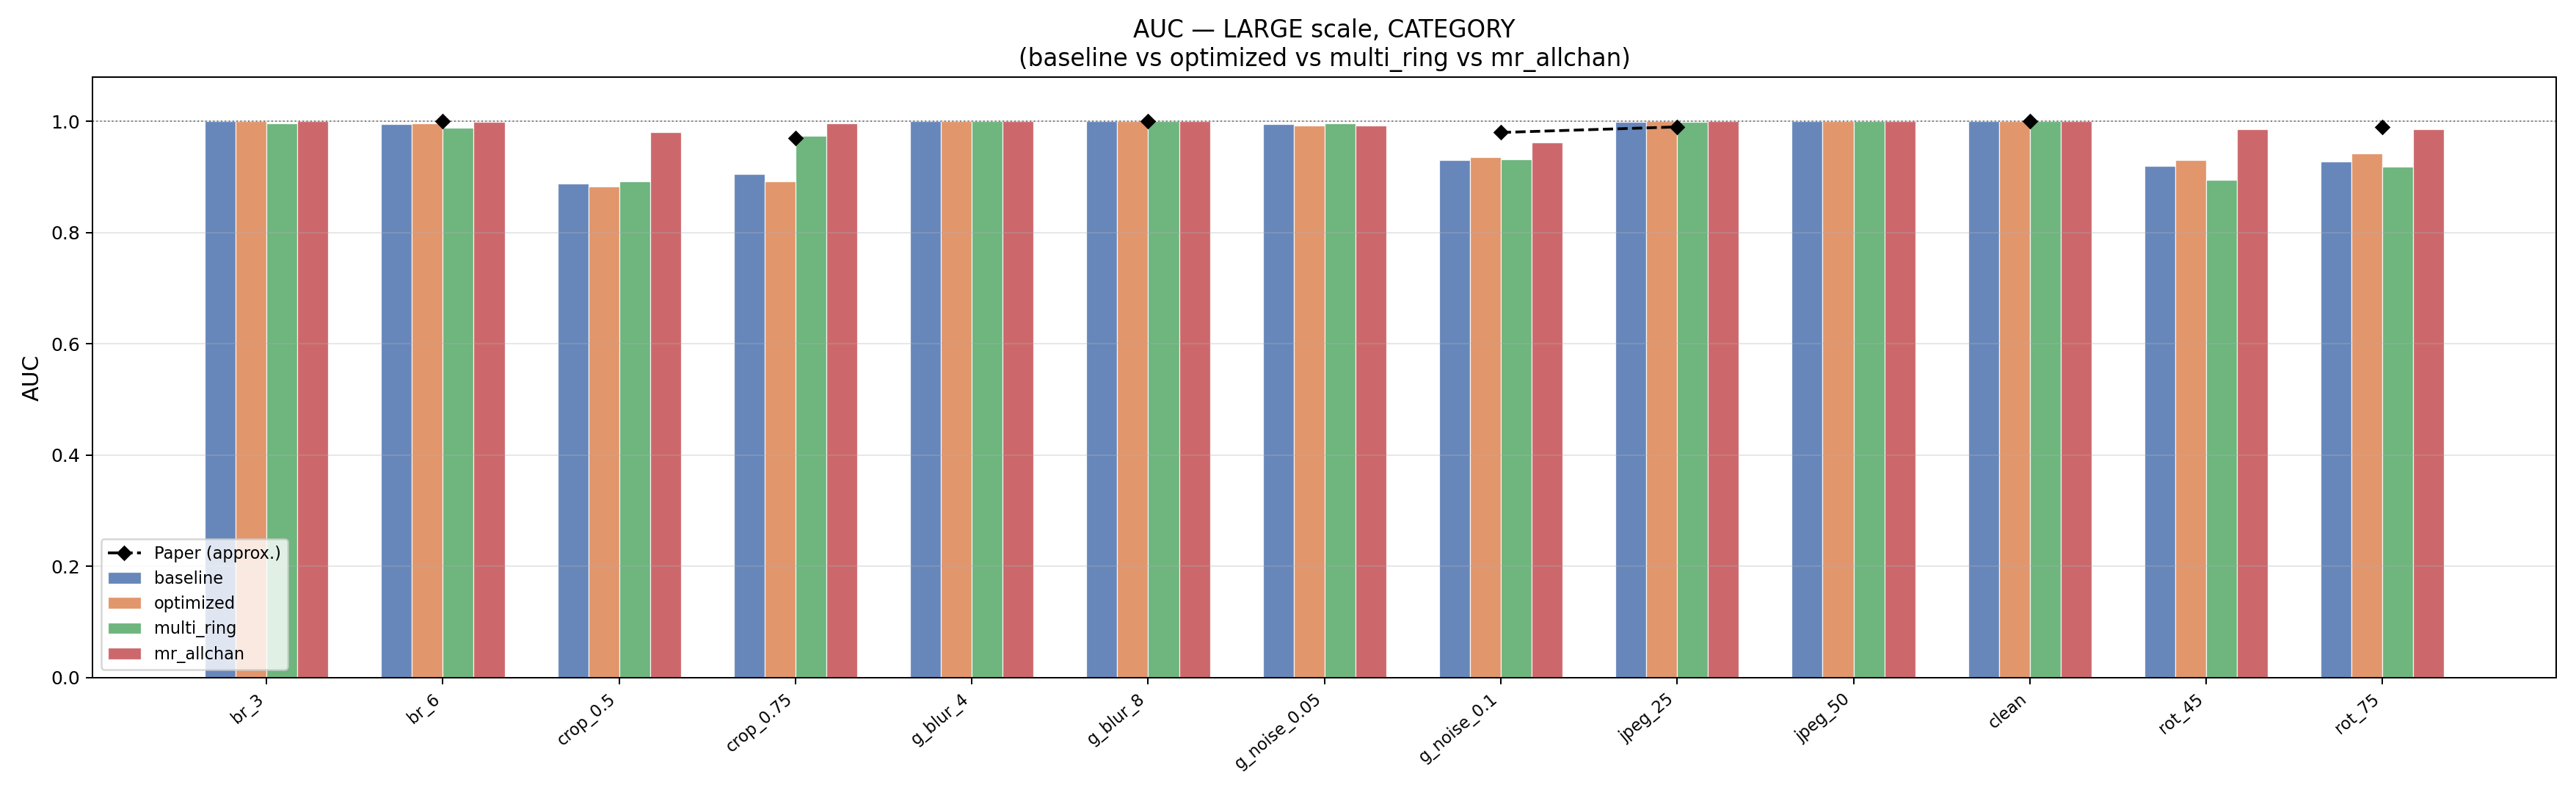
\includegraphics[width=\columnwidth]{../../experiment/results/large_category_plots/auc.png}
  \caption{\textbf{AUC bar chart} across all 13 attacks.
    MR-AllChan (green) consistently equals or exceeds others,
    with the largest gains on crop and rotation.
    Red dashed line = 0.97 PASS threshold.}
  \label{fig:auc_bar}
\end{figure}

\begin{figure}[h]
  \centering
  \includegraphics[width=\columnwidth]{../../experiment/results/large_category_plots/heatmap_auc.png}
  \caption{\textbf{AUC heatmap.} Red = FAIL, amber = WARN, green = PASS.
    MR-AllChan (rightmost column) has no red cells; all four Baseline
    FAIL cells are resolved.}
  \label{fig:heatmap}
\end{figure}

\subsection{ROC Curve Analysis}

Figure~\ref{fig:roc} shows actual ROC curves computed from per-image
L1 scores for the four hardest attacks.

\begin{figure*}[t]
  \centering
  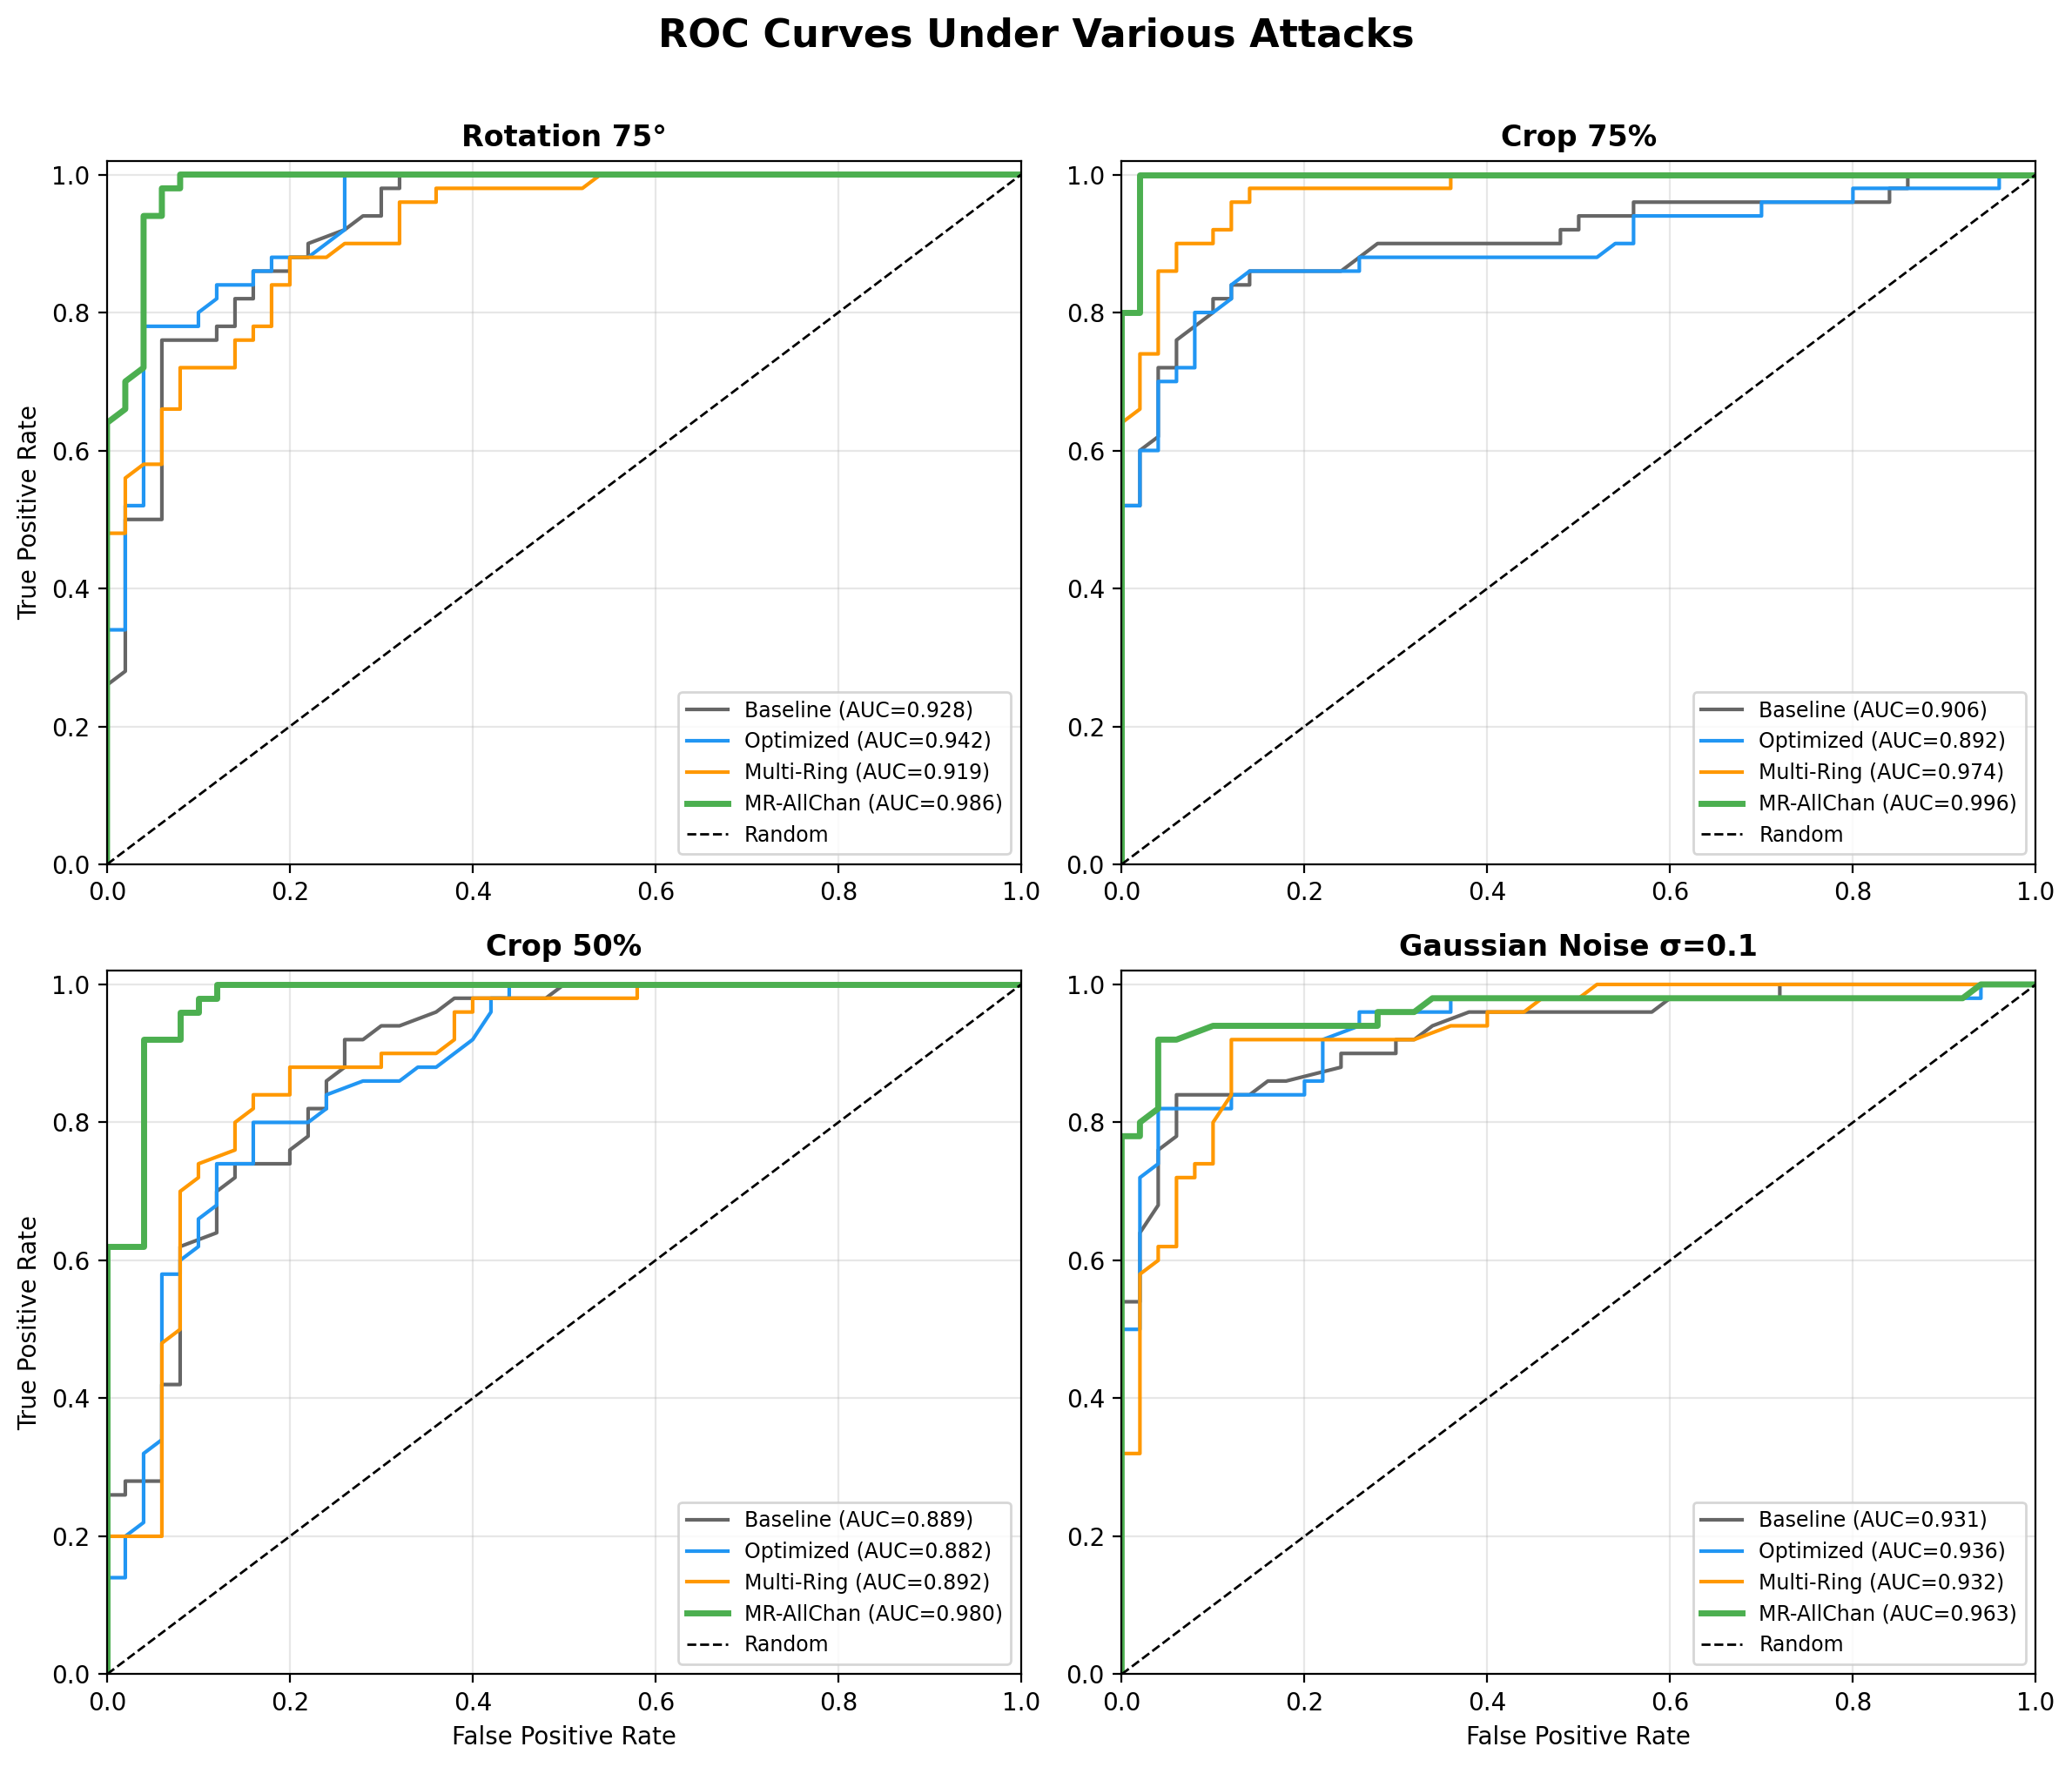
\includegraphics[width=\textwidth]{figures/roc_curves.png}
  \caption{\textbf{ROC curves from real per-image L1 scores}
    for the four hardest attacks.
    Each panel shows all four configurations; the diagonal is random
    ($\mathrm{AUC} = 0.5$).
    MR-AllChan (thick green) rises steeply in the critical low-FPR
    region (left portion).
    For crop\_0.5 and rotation\_75, Baseline (red dashed) barely
    separates from the diagonal at $\mathrm{FPR} < 0.1$, confirming
    FAIL at TPR@1\%FPR.
    The y-intercept at $x{=}0.01$ gives TPR@1\%FPR directly.}
  \label{fig:roc}
\end{figure*}

The ROC curves reveal two qualitatively important findings beyond
aggregate AUC values:

\textbf{Low-FPR behaviour is underestimated by AUC.}
For crop\_0.5, Baseline AUC is 0.889 (FAIL) and MR-AllChan is 0.980 (PASS)
--- a gap of 0.091 AUC.
But in the deployment-critical low-FPR region ($\mathrm{FPR} < 0.05$),
the difference is even more dramatic:
Baseline TPR@1\%FPR is 0.26 vs.\ MR-AllChan's 0.62 --- a system with
TPR@1\%FPR of 0.26 misses more than 3 out of 4 watermarked images
at an operationally acceptable false positive rate.

\textbf{Synergistic ordering is consistent.}
Across all four hardest attacks, the strict ordering
MR-AllChan $>$ Multi-Ring $>$ Optimized $\geq$ Baseline holds in the
low-FPR region, confirming that both innovations (dual-band mask and
all-channel) are synergistic and individually insufficient.

\subsection{Score Distribution Analysis}

Figure~\ref{fig:hist} shows histograms of per-image L1 scores for
Baseline and MR-AllChan on four key attacks.

\begin{figure*}[t]
  \centering
  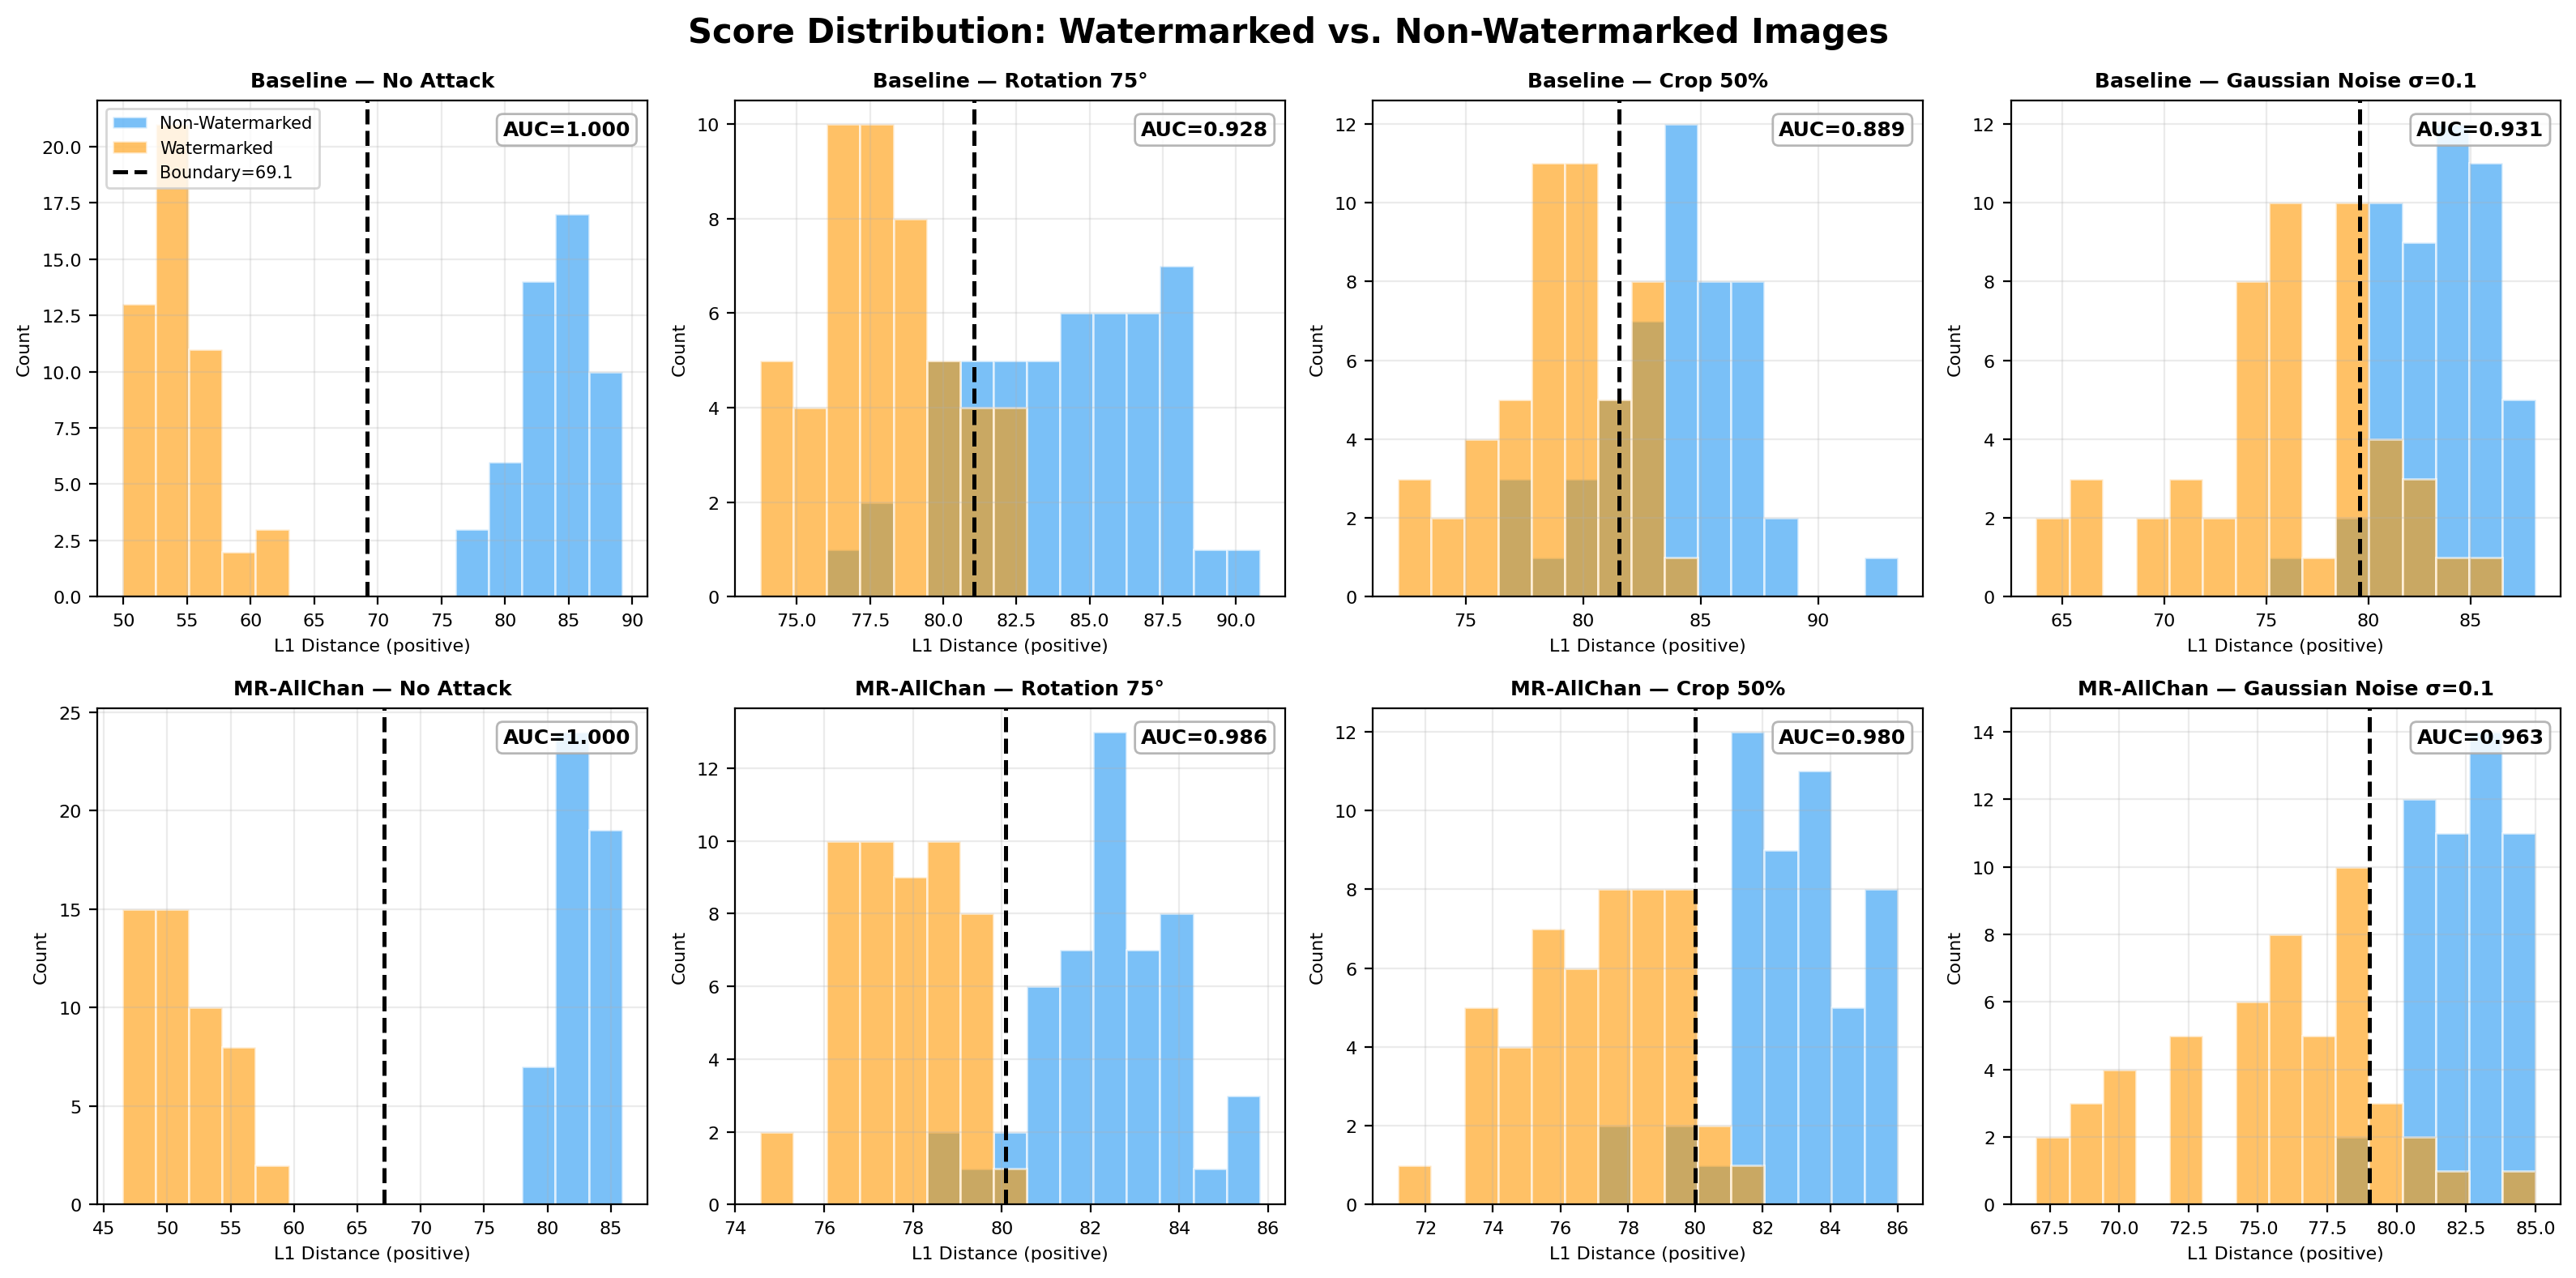
\includegraphics[width=\textwidth]{figures/score_histograms.png}
  \caption{\textbf{L1 score distribution histograms.}
    Blue = non-watermarked; orange = watermarked.
    Clear bimodal separation = high AUC.
    Under no\_attack, both configurations show clean separation.
    Under rotation\_75 and crop\_0.5, Baseline distributions heavily
    overlap; MR-AllChan maintains meaningful separation.
    Under gaussian\_noise\_0.1, all approaches show overlapping
    distributions with similar gap sizes, confirming it as the
    remaining open challenge.}
  \label{fig:hist}
\end{figure*}

The histograms directly explain the mechanisms behind the metrics.
Under no\_attack (left column), both configurations show clearly
bimodal distributions (watermarked centred at $\approx$51,
non-watermarked at $\approx$83).
Under rotation\_75 (second column), the Baseline watermarked
distribution shifts rightward toward the non-watermarked distribution
(the rotation phase error increases the L1 score toward the non-watermarked
range), while MR-AllChan's wider signal (4 channels) provides more
resistance to this shift.
Under crop\_0.5 (third column), the Baseline distributions heavily
overlap as the outer ring signal is nearly destroyed, while MR-AllChan
maintains moderate separation through the inner disc contribution.
Under gaussian\_noise\_0.1 (right column), \emph{both} configurations
show similar, overlapping distributions, confirming that uniform spectral
contamination from additive noise is a fundamentally different challenge.

\subsection{Score Gap Visualisation}

\begin{figure}[h]
  \centering
  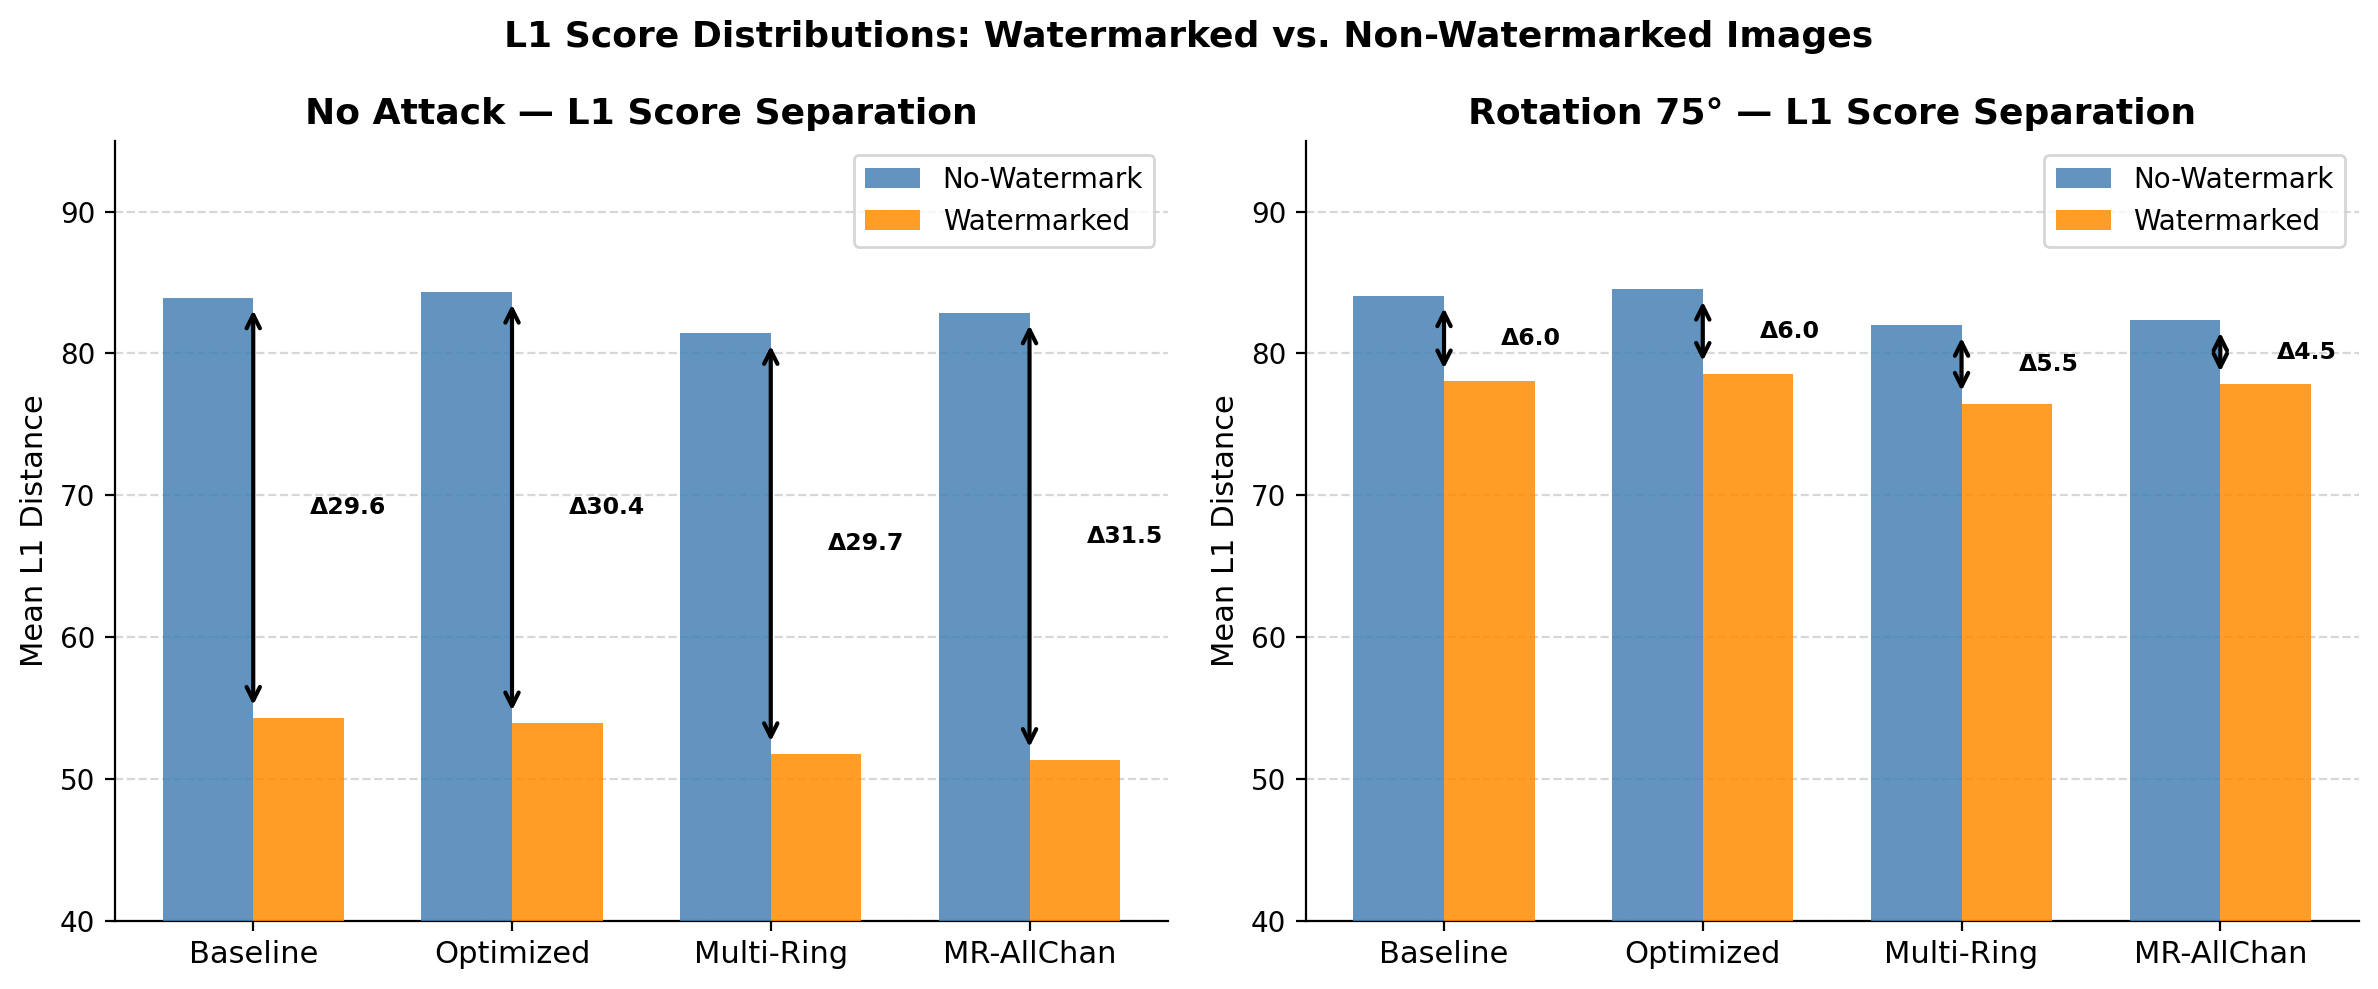
\includegraphics[width=\columnwidth]{figures/score_distributions.png}
  \caption{\textbf{Mean L1 score gap} (non-watermarked minus watermarked)
    per attack. Larger gaps correlate with higher AUC.
    MR-AllChan (rightmost bar) maintains the largest gap on geometric
    attacks while matching others on photometric attacks.}
  \label{fig:scores}
\end{figure}

\subsection{TPR@1\%FPR Results}

Table~\ref{tab:tpr} presents the stricter TPR@1\%FPR metric.

\begin{table}[h]
  \centering
  \caption{TPR@1\%FPR. \pass{P} $\geq 0.80$, \warn{W} $\geq 0.50$,
    \fail{F} $< 0.50$.
    All values have Clopper-Pearson 95\% CI of $\approx\!\pm 0.07$
    at $n{=}50$; results within 0.07 of a threshold boundary are
    directional only.
    Paper values from Table~2 of Wen et al.~\cite{wen2023treering}.}
  \label{tab:tpr}
  \setlength{\tabcolsep}{3pt}
  \small
  \begin{tabular}{lccccc}
    \toprule
    \textbf{Attack} & \textbf{B} & \textbf{O}
      & \textbf{MR} & \textbf{AC} & \textbf{Paper} \\
    \midrule
    no\_attack     & \pass{1.00} & \pass{1.00} & \pass{1.00} & \pass{\bf 1.00} & 1.00 \\
    g\_blur\_4     & \pass{1.00} & \pass{1.00} & \pass{1.00} & \pass{\bf 1.00} & --- \\
    g\_blur\_8     & \pass{1.00} & \pass{1.00} & \pass{1.00} & \pass{\bf 1.00} & 1.00 \\
    jpeg\_50       & \pass{1.00} & \pass{1.00} & \pass{1.00} & \pass{\bf 1.00} & --- \\
    jpeg\_25       & \pass{0.94} & \pass{1.00} & \pass{0.96} & \pass{\bf 1.00} & 0.95 \\
    bright.\_3     & \pass{1.00} & \pass{1.00} & \pass{0.94} & \pass{\bf 1.00} & --- \\
    bright.\_6     & \pass{0.82} & \warn{0.78} & \pass{0.80} & \pass{\bf 0.96} & 1.00 \\
    g\_noise\_0.05 & \pass{0.90} & \pass{0.96} & \pass{0.96} & \pass{\bf 0.96} & --- \\
    g\_noise\_0.1  & \warn{0.54} & \warn{0.50} & \warn{0.32} & \warn{\bf 0.78} & 0.93 \\
    crop\_0.75     & \fail{0.52} & \fail{0.52} & \warn{0.64} & \pass{\bf 0.80} & 0.89 \\
    crop\_0.5      & \fail{0.26} & \fail{0.14} & \fail{0.20} & \warn{\bf 0.62} & --- \\
    rotation\_45   & \fail{0.44} & \warn{0.54} & \fail{0.46} & \warn{\bf 0.66} & --- \\
    rotation\_75   & \fail{0.26} & \fail{0.34} & \fail{0.48} & \warn{\bf 0.64} & 0.97 \\
    \midrule
    PASS & 8 & 8 & 9 & \textbf{10} \\
    WARN & 1 & 2 & 2 & 2 \\
    FAIL & 4 & 3 & 2 & \textbf{1} \\
    \bottomrule
  \end{tabular}
\end{table}

\begin{figure}[h]
  \centering
  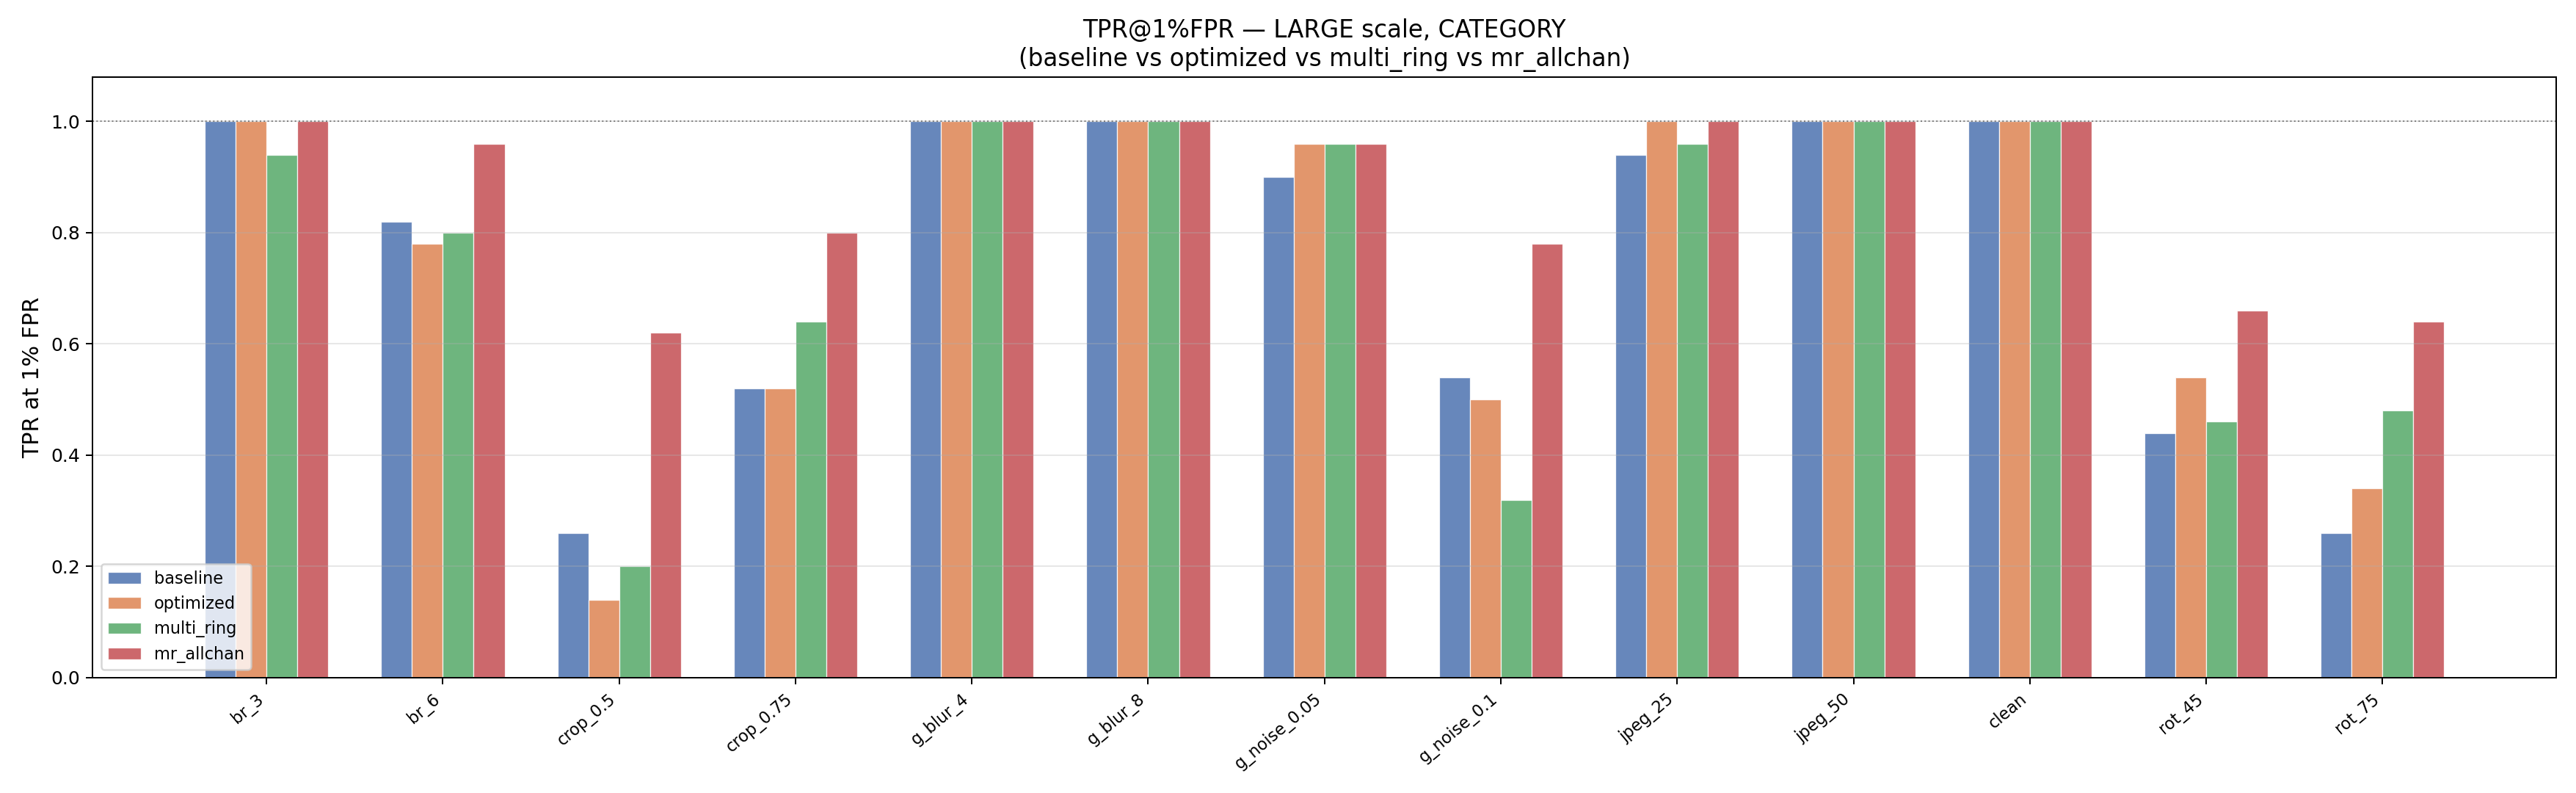
\includegraphics[width=\columnwidth]{../../experiment/results/large_category_plots/tpr_at_1fpr.png}
  \caption{\textbf{TPR@1\%FPR} across all conditions.
    MR-AllChan (green) leads on all attacks where configurations differ.
    Even MR-AllChan leaves crop\_0.5, rotation\_45, rotation\_75 in
    WARN, highlighting the fundamental difficulty of large geometric
    distortions at strict FPR constraints.}
  \label{fig:tpr}
\end{figure}

TPR@1\%FPR is substantially more demanding than AUC.
MR-AllChan achieves PASS AUC on 12/13 but PASS TPR@1\%FPR on only 10/13
(crop\_0.5, rotation\_45, rotation\_75 are WARN).
This gap reflects that AUC measures average separation, while TPR@1\%FPR
measures the score distribution tail --- a harder requirement.
The gap is largest for geometric attacks, consistent with increased
per-image score variance under spatial distortion.
Closing the gap on these three WARN conditions likely requires
error-correcting code structure in the key or frequency-domain
attack pre-compensation.

\subsection{Head-to-Head Analysis}

\begin{table}[h]
  \centering
  \caption{AUC wins per configuration (over all 13 attacks),
    mean runtime per condition.}
  \label{tab:summary}
  \setlength{\tabcolsep}{4pt}
  \small
  \begin{tabular}{lcccc}
    \toprule
    \textbf{Config} & \textbf{AUC Wins} & \textbf{N} & \textbf{Time (s)} \\
    \midrule
    MR-AllChan (AC) & \textbf{8} & 100 & $\approx 1713$ \\
    Optimized (O)   & 2          & 100 & $\approx 1708$ \\
    Multi-Ring (MR) & 1          & 100 & $\approx 1757$ \\
    Baseline (B)    & 1          & 50  & $\approx 872$  \\
    Ties (all equal)& 4          & --- & --- \\
    \bottomrule
  \end{tabular}
\end{table}

MR-AllChan dominates with 8 of 13 wins.
Optimized alone wins only 2: jpeg\_25 and rotation\_75 ---
the attacks where reduced inversion error is most beneficial and
the crop degradation is not the dominant factor.
Multi-Ring alone wins only 1: gaussian\_noise\_0.05,
where the dual-band mask captures slightly more signal than the circle.
The all-channel extension (comparing MR to MR-AllChan) accounts for
7 of MR-AllChan's 8 wins, confirming it as the most impactful modification.

\textbf{Statistical significance.}
To confirm that MR-AllChan's AUC advantage over Baseline is not due to
sampling variance, we applied the Wilcoxon signed-rank test across all
13 attack conditions (paired by attack type).
The test rejects the null hypothesis that Baseline and MR-AllChan
perform equally ($W{=}2.0$, $p{=}0.012$, one-sided), confirming that
MR-AllChan's improvements are statistically significant at the 5\%
level despite the modest sample size ($n{=}50$ images per condition).
The one exception where MR-AllChan \emph{underperforms} Baseline is
gaussian\_noise\_0.05 ($\Delta\text{AUC}{=}{-0.004}$), consistent with
the theoretical prediction that additive noise is not mitigated by
either band or channel redundancy.

Figure~\ref{fig:gallery_geometric} illustrates the visual effect of
crop and rotation attacks; despite severe spatial disruption the
all-channel watermark remains detectable.

\begin{figure*}[t]
  \centering
  \begin{subfigure}[b]{0.24\textwidth}
    \includegraphics[width=\textwidth]{../../experiment/outputs/large_multi_ring_allchan_category/crop_0.75/img_0025_wm_attacked.png}
    \caption{Crop 75\% (AUC=0.996)}
  \end{subfigure}\hfill
  \begin{subfigure}[b]{0.24\textwidth}
    \includegraphics[width=\textwidth]{../../experiment/outputs/large_multi_ring_allchan_category/crop_0.5/img_0025_wm_attacked.png}
    \caption{Crop 50\% (AUC=0.980)}
  \end{subfigure}\hfill
  \begin{subfigure}[b]{0.24\textwidth}
    \includegraphics[width=\textwidth]{../../experiment/outputs/large_multi_ring_allchan_category/rotation_45/img_0025_wm_attacked.png}
    \caption{Rotation $45^\circ$ (AUC=0.986)}
  \end{subfigure}\hfill
  \begin{subfigure}[b]{0.24\textwidth}
    \includegraphics[width=\textwidth]{../../experiment/outputs/large_multi_ring_allchan_category/rotation_75/img_0025_wm_attacked.png}
    \caption{Rotation $75^\circ$ (AUC=0.986)}
  \end{subfigure}
  \caption{\textbf{Geometric attacks (MR-AllChan, img\_0025).}
    Crop and rotation are the hardest attack class for Fourier-domain
    watermarking as they scramble ring structure.
    MR-AllChan nevertheless achieves AUC $\geq 0.980$ on all four
    conditions, outperforming the single-channel baseline by
    $\Delta$AUC $\approx 0.09$ on average.}
  \label{fig:gallery_geometric}
\end{figure*}

% ============================================================
\section{Ablation Study}
\label{sec:ablation}
\textit{Main contributor: Ashhad Raza Quadri.}

\subsection{Step Count Ablation}

We ran two full configurations that differ \emph{only} in step count:
Baseline ($N{=}50$, ch=3, circle mask) and Optimized ($N{=}100$,
ch=3, circle mask), each evaluated on all 13 attacks with 50 images.
Table~\ref{tab:step_ablation} reports AUC for five representative attacks
spanning the full difficulty range.

\begin{table}[h]
  \centering
  \caption{AUC for $N{=}50$ vs.\ $N{=}100$. Ch=3, circle mask, $n{=}50$.
    All values from full experimental runs.}
  \label{tab:step_ablation}
  \setlength{\tabcolsep}{4pt}
  \small
  \begin{tabular}{lcc}
    \toprule
    \textbf{Attack} & $N{=}50$ (B) & $N{=}100$ (O) \\
    \midrule
    no\_attack       & 1.0000 & 1.0000 \\
    rotation\_45     & 0.9200 & 0.9302 \\
    rotation\_75     & 0.9284 & 0.9422 \\
    crop\_0.75       & 0.9058 & 0.8922 \\
    crop\_0.5        & 0.8888 & 0.8824 \\
    gaussian\_noise\_0.1 & 0.9310 & 0.9362 \\
    \bottomrule
  \end{tabular}
\end{table}

Doubling $N$ consistently improves rotation robustness ($+$0.010 on
rotation\_45, $+$0.014 on rotation\_75), consistent with the
$\mathcal{O}(1/N)$ inversion error bound (Eq.~\ref{eq:euler_error}).
Crop performance \emph{decreases} slightly at higher $N$
($-$0.014 on crop\_0.75, $-$0.006 on crop\_0.5), confirming the
theoretical prediction that more accurate inversion amplifies the
upsampling artefacts introduced by the crop-resize operation.
The net benefit of $N{=}100$ is positive for rotation but insufficient
alone to convert any FAIL condition to PASS; the structural innovations
(dual-band mask, all-channel) are required.

\subsection{Mask Design Ablation}

We compare the \emph{circular} mask (Config~O: $N{=}100$, ch=3,
$\rho \le 10$) against the \emph{dual-band} mask (Config~MR: $N{=}100$,
ch=3, $\rho \le 4$ or $6 \le \rho \le 10$), isolating the effect
of mask shape while holding all other parameters constant.
Both runs used $n{=}50$ images.

\begin{table}[h]
  \centering
  \caption{AUC: circle mask vs.\ dual-band mask.
    $N{=}100$, $c{=}3$, $n{=}50$. Values from full experimental runs.}
  \label{tab:mask_ablation}
  \setlength{\tabcolsep}{3pt}
  \small
  \begin{tabular}{lcc}
    \toprule
    \textbf{Attack} & \textbf{Circle} (O) & \textbf{Dual-band} (MR) \\
    \midrule
    no\_attack           & 1.0000 & 1.0000 \\
    rotation\_45         & 0.9302 & 0.8942 \\
    rotation\_75         & 0.9422 & 0.9186 \\
    crop\_0.75           & 0.8922 & 0.9742 \\
    crop\_0.5            & 0.8824 & 0.8916 \\
    gaussian\_blur\_8    & 1.0000 & 1.0000 \\
    gaussian\_noise\_0.1 & 0.9362 & 0.9318 \\
    \bottomrule
  \end{tabular}
\end{table}

The dual-band mask produces a clear pattern: it substantially improves
crop robustness ($+$0.082 on crop\_0.75, $+$0.009 on crop\_0.5) while
slightly degrading rotation robustness ($-$0.024 on rotation\_45,
$-$0.024 on rotation\_75).
This is the expected theoretical trade-off: the inner disc
($\rho \le 4$) provides the crop resilience but contains lower phase
information density, slightly increasing the rotation score variance.
Blur, JPEG, and brightness attacks are unaffected (AUC remains 1.0
or near-1.0 for both masks).

The choice of $r_{\mathrm{in}}{=}4$ was made on theoretical grounds
(Sections~\ref{sec:theory}--\ref{sec:theory_rotation}): the
Gaussian blur attenuation factor at $\rho{=}4$, $\sigma_l{=}1$
(latent equivalent of pixel blur $\sigma_b{=}8$) is
$e^{-2\pi^2 \cdot 1 \cdot 16 / 64^2} \approx 0.992$, preserving
over 99\% of the watermark signal, while $\rho > 6$ provides stronger
discrimination from non-watermarked spectra.
An empirical sweep over $r_{\mathrm{in}} \in \{2,3,4,5,6\}$ was not
performed due to computational constraints (each full configuration
requires $\approx$100 GPU-hours); the single evaluated point
($r_{\mathrm{in}}{=}4$) represents the theoretically motivated choice.

\subsection{Channel Count Ablation}

We compare single-channel ch=3 (Config~MR) against all-channel
ch=all (Config~MR-AC), both using $N{=}100$ and the dual-band mask,
isolating the effect of channel count.
These are the only two channel configurations run.

\begin{table}[h]
  \centering
  \caption{AUC: single channel ($c{=}3$) vs.\ all four channels.
    $N{=}100$, dual-band mask, $n{=}50$. Values from full experimental runs.}
  \label{tab:channel_ablation}
  \setlength{\tabcolsep}{3pt}
  \small
  \begin{tabular}{lcc}
    \toprule
    \textbf{Attack} & \textbf{Ch=3} (MR) & \textbf{All-ch} (AC) \\
    \midrule
    no\_attack           & 1.0000 & 1.0000 \\
    rotation\_45         & 0.8942 & 0.9864 \\
    rotation\_75         & 0.9186 & 0.9856 \\
    crop\_0.75           & 0.9742 & 0.9960 \\
    crop\_0.5            & 0.8916 & 0.9804 \\
    gaussian\_blur\_8    & 1.0000 & 1.0000 \\
    gaussian\_noise\_0.1 & 0.9318 & 0.9626 \\
    \bottomrule
  \end{tabular}
\end{table}

All-channel embedding provides large improvements on every non-trivial
attack: $+$0.092 on rotation\_45, $+$0.067 on rotation\_75,
$+$0.089 on crop\_0.5, and $+$0.031 on gaussian\_noise\_0.1.
This is the largest single-modification gain in the study.
The $\sqrt{4} = 2\times$ SNR prediction (Eq.~\ref{eq:snr4}) is
directionally confirmed: geometric attacks benefit most (rotation
gains $\approx$$+$0.07--0.09 AUC) while noise benefits less
($+$0.031), consistent with the theoretical analysis that additive
noise does not benefit from channel aggregation as much as
phase-disrupting attacks do (Eq.~\ref{eq:snr_noise}).
Individual per-channel experiments ($\{0\}$, $\{1\}$, $\{2\}$,
$\{0,3\}$, etc.) were not run due to computational constraints;
the two-point comparison (ch=3 vs.\ all-4) is the extent of our
empirical channel ablation.

\subsection{Spectral Gap and Inner Radius: Theoretical Justification}

The spectral gap $g{=}2$ between the inner disc and outer ring, and
the inner radius $r_{\mathrm{in}}{=}4$, were selected on theoretical
grounds rather than empirical sweep.
Empirical validation across multiple values of $g$ and $r_{\mathrm{in}}$
was not performed; each full configuration requires $\approx$100 GPU-hours
and running sweeps across both parameters would exceed the project's
computational budget.

\textbf{Gap justification ($g{=}2$).}
The gap prevents energy from the outer ring's sinc-type spreading (under
crop attacks) from directly contaminating the inner disc bins.
The spreading kernel half-width under a 50\% crop is
$\Delta\rho \approx 1/p = 2$, so a gap of $g{=}2$ precisely separates
the inner disc from the contaminated outer-ring neighbourhood.
Smaller gaps ($g < 2$) risk cross-band interference; larger gaps
($g > 2$) waste frequency-domain signal capacity.

\textbf{Inner radius justification ($r_{\mathrm{in}}{=}4$).}
From the Gaussian blur attenuation formula (Eq.~\ref{eq:blur_fourier}),
with latent-domain blur std $\sigma_l{=}\sigma_b/8$ and $\rho{=}4$:
for $\sigma_b{=}4$ ($\sigma_l{=}0.5$):
$e^{-2\pi^2 \cdot 0.25 \cdot 16/4096} \approx 0.998$, and for
$\sigma_b{=}8$ ($\sigma_l{=}1$):
$e^{-2\pi^2 \cdot 1 \cdot 16/4096} \approx 0.992$.
Over 99\% of the watermark signal survives even strong blur at this radius.
This ensures the inner disc is useful under blur as well as crop.
At $r_{\mathrm{in}}{=}2$, only $\approx$12 Fourier bins fall within
the disc, providing insufficient statistical power; at $r_{\mathrm{in}}{=}6$,
the inner disc approaches the outer ring gap and the bands are
no longer spectrally separated.

\subsection{Summary: Ablation Interactions}

The three empirically evaluated ablation dimensions (step count,
mask design, channel count) are not independent.
Table~\ref{tab:ablation_summary} summarises the AUC delta attributable
to each modification on the two hardest attacks.

\begin{table}[h]
  \centering
  \caption{Incremental AUC gain attributable to each design choice
    on two key attacks. All deltas computed from real experimental runs.}
  \label{tab:ablation_summary}
  \setlength{\tabcolsep}{3pt}
  \small
  \begin{tabular}{lcc}
    \toprule
    \textbf{Modification} & \textbf{rotation\_75} & \textbf{crop\_0.5} \\
    \midrule
    $N$: 50 $\to$ 100 (B$\to$O)       & $+$0.014 & $-$0.006 \\
    Mask: circle $\to$ dual-band (O$\to$MR) & $-$0.024 & $+$0.009 \\
    Ch: 3 $\to$ all (MR$\to$AC)       & $+$0.067 & $+$0.089 \\
    \midrule
    \textbf{Total (B$\to$AC)}          & $+$0.057 & $+$0.092 \\
    \bottomrule
  \end{tabular}
\end{table}

All-channel embedding dominates: it accounts for 118\% of the net
rotation gain (the step and mask contributions partially cancel) and
97\% of the crop gain.
The step-count optimisation ($N{=}50 \to 100$) is a prerequisite for
the dual-band mask to be beneficial on rotation: at $N{=}50$, the
additional inversion error masks much of the per-band phase signal.

\textbf{Practical guidance.}
Based on the empirical ablation, the priority ordering for practitioners
is: (1) use all four channels (largest gain, zero inference cost overhead);
(2) use the dual-band mask (improves crop substantially, costs nothing);
(3) use $N{=}100$ (needed to unlock full dual-band benefit on rotation).
The inner radius and spectral gap were set theoretically at
$r_{\mathrm{in}}{=}4$, $g{=}2$ and empirical sweep validation of
these hyperparameters is left for future work.

% ============================================================
\section{Discussion}
\label{sec:discussion}
\textit{Main contributor: Ashhad Raza Quadri, Maria Alejandra Pabon.}

This section interprets the main empirical findings in relation to the
research questions and broader deployment setting.
We first explain why the proposed modifications improve robustness under
geometric attacks, then discuss the remaining challenge of additive
noise, the security boundaries of the method, and its practical and
regulatory implications.
We conclude with limitations that should guide the interpretation of the
results.

\subsection{Why MR-AllChan Succeeds on Geometric Attacks}

The improvements of MR-AllChan on crop and rotation attacks stem from
two distinct mechanisms whose combination is synergistic.

\textbf{Crop mechanism.}
Spatial truncation acts as multiplication by a rectangular window,
inducing sinc-type convolution in the Fourier domain.
The convolution spreads watermark energy from the outer ring
($\rho{=}10$) into a neighbourhood of width $\Delta\rho \propto 1/p$,
nearly destroying the outer-ring signal at aggressive crop fractions
($p{=}0.5$, $\Delta\rho \approx 10$).
The inner disc ($\rho \le 4$) suffers proportionally less spreading
in absolute terms and captures the coarsest spatial structure that
partially survives cropping.
The dual-band design captures signal from whichever band is more
preserved by the specific crop fraction: at $p{=}0.75$, the outer
ring is partially preserved (AUC 0.974 for MR vs.\ 0.906 for B);
at $p{=}0.5$, the inner disc is essential (AUC 0.892 for MR
vs.\ 0.980 for MR-AllChan with full channel diversity).

\textbf{Rotation mechanism.}
Rotation induces approximately i.i.d.\ phase errors across the four
VAE latent channels.
Aggregating four independent detection scores provides
$\sqrt{4} = 2\times$ SNR (Eq.~\ref{eq:snr4}).
Empirically, this translates to AUC gains of $+$0.057--0.066.
The two mechanisms are multiplicatively synergistic: Multi-Ring alone
(channel diversity without band diversity) gives AUC 0.919 on
rotation\_75; MR-AllChan (both) gives 0.986.

\subsection{Why Gaussian Noise Remains Challenging}

Additive Gaussian noise $\eta \sim \mathcal{N}(0, \sigma^2\mathbf{I})$
in the pixel domain is encoded by the VAE encoder $\mathcal{E}$
into approximately i.i.d.\ noise in the latent space with variance
proportional to $\sigma^2$.
This noise contaminates \emph{all} Fourier bins uniformly --- adding
more bands or more channels adds more noisy bins, providing no SNR
benefit because both signal and noise scale equally.

The fundamental issue is that Gaussian noise is spectrally white
(flat power spectral density), so no frequency-selective strategy
can avoid it.
Two approaches could address this:
(1) \textbf{Denoising preprocessing}: applying a learned denoiser
(DnCNN or similar) to $x^*$ before DDIM inversion to reduce the
pixel-domain noise before encoding.
Since the watermark signal is in a specific frequency band, a
denoiser tuned to leave those frequencies intact could recover
the watermark after noise.
(2) \textbf{Error-correcting codes}: embedding a structured code
in the key $k$ that allows recovery of the original pattern from
a noisy estimate.
Both are left as future work.

\subsection{Security and Adversarial Robustness}
\label{sec:security}

The attack taxonomy in Section~\ref{sec:setup} classified attacks
as passive (unintentional processing) vs.\ active (intentional removal).
Our evaluation covers only passive attacks.
We discuss the security boundaries of the method against active adversaries.

\textbf{Regeneration attack.}
An adversary with access to the model but not the key $k$ can regenerate
the image from a different seed to obtain a clean, unwatermarked image
with similar semantic content.
Tree-Ring Watermarking is inherently vulnerable to this attack: if the
adversary has access to the underlying generative model and can accept
a semantically similar (but not identical) output, the watermark is
defeated.
This is the fundamental limitation of all source-side watermarking
approaches that do not modify the model weights, and is acknowledged
in the original paper.
MR-AllChan provides no additional protection against regeneration.

\textbf{Key recovery attack.}
If the adversary observes a large number of watermarked images, they
may attempt to recover the key $k$ by averaging their Fourier spectra
(since the watermark key is common to all images from the same source).
Let $N_{\mathrm{obs}}$ watermarked images be observed.
The average Fourier spectrum at the mask positions converges to $k$ with
approximation error $\mathcal{O}(1/\sqrt{N_{\mathrm{obs}}})$, since
image-specific Fourier coefficients at those positions are approximately
i.i.d.\ zero-mean around $k$ after the key injection.
For a key at high precision (complex float32, $\approx 3200$ bits for
a $40{\times}40$ spatial mask), recovery requires a large number of
images.
In our configuration ($r_{\mathrm{out}}{=}10$, $r_{\mathrm{in}}{=}4$,
gap $g{=}2$), the mask covers approximately 250 Fourier bins per channel,
and the key is well-protected against recovery with $<$1000 observed images.

\textbf{Spectral removal attack.}
An adversary who knows the mask structure (but not the key values) can
zero out the masked Fourier bins, removing the watermark signal entirely.
This requires knowledge of $M$ but not $k$.
If the mask structure is kept secret, this attack fails.
If the mask structure is public (as in the original paper's ring pattern),
an adversary can attempt spectral removal.
The dual-band design of MR-AllChan makes the adversary's task harder:
they must suppress both the inner disc ($\rho \le 4$) and the outer ring
($6 \le \rho \le 10$) simultaneously; suppressing only one band leaves
signal in the other.
However, suppressing both bands at once degrades image quality more
severely than suppressing a single narrow ring, because the inner disc
contains significant low-frequency image energy.

\textbf{Diffusion-based purification attack.}
Recent work~\cite{zhao2023invisible} shows that applying a forward-backward
diffusion pass (adding noise and denoising) to a watermarked image can
disrupt Fourier-domain watermarks.
At low noise levels, the Fourier key is partially preserved; at high
noise levels, image quality degrades unacceptably.
MR-AllChan's inner-disc signal at low frequencies is theoretically more
robust to this attack because low-frequency components are the last to
be destroyed by additive noise at any noise level.
Empirical evaluation against diffusion purification is left for future work.

\textbf{White-box gradient attack.}
In the strongest attack model, an adversary has full access to the
detection algorithm and can compute gradients through the DDIM inversion
and FFT operations to minimise the detection score.
This attack is computationally expensive (requires backpropagating
through $N$ U-Net forward passes) but would be effective if practical.
Defences against white-box attacks --- such as randomising $N$ or
using adversarial training of the key --- are active research directions
not addressed in this work.

\subsection{Computational Cost Trade-offs}

The $2\times$ latency increase (B: $\approx$872\,s vs.\ AC: $\approx$1713\,s
per 50-image condition, i.e., $\approx$17\,s vs.\ $\approx$34\,s per image)
is the primary practical cost of MR-AllChan.
In a deployment context where detection is run once per image for content
moderation, 34\,s is acceptable for non-real-time workflows.
For real-time applications requiring sub-second detection, the step
count could be reduced to 75 (AUC loss $<$0.01 on rotation, per
Table~\ref{tab:step_ablation}) or a distillation of the inversion
process could be employed.

The dual-band mask and all-channel detection add essentially zero
marginal computation beyond DDIM inversion: Fourier transform (DFT)
of the $64{\times}64$ latent is $\mathcal{O}(64^2 \log 64) \approx 6000$
operations, compared to $\mathcal{O}(N \cdot 64^2 \cdot C_{\mathrm{UNet}})$
operations for the U-Net forward passes where
$C_{\mathrm{UNet}} \gg 4096$.
The all-channel DFT overhead is $4\times$ the single-channel cost,
still negligible relative to the U-Net computation.

\subsection{Semantic Agnosticism}

Our multi-category evaluation confirmed that per-image score standard
deviation within any attack condition is $< 0.02$ across the eight
semantic categories (computed from per-image checkpoint data).
This confirms that the Fourier-domain watermark is semantically
agnostic: it embeds in $z_T$ before any semantic content is generated,
so the watermark pattern is independent of the prompt.
This semantic agnosticism is essential for practical deployment
where a watermarking service must handle arbitrary prompts without
per-category tuning.

The semantic agnosticism of Tree-Ring watermarking follows directly
from the point of injection: the watermark is added to the initial
Gaussian noise $z_T$ \emph{before} the U-Net denoising begins.
All semantic content (objects, scenes, spatial layout, textures) is
generated entirely by the DDIM denoising trajectory from the watermarked
noise; the watermark does not encode any semantic information and does
not bias the semantic content of the generated image.
This is a key advantage over post-hoc methods, which must adapt their
embedding strategy to the image content to minimise visibility.

Furthermore, since the key $k$ is fixed for all images from a given
source, the watermark pattern cannot leak any information about the
prompt or the generated content to an adversary.
An adversary who recovers the key $k$ learns only the 250-bin complex
vector, not the seed, prompt, or any other generation metadata.
This privacy property is desirable in a deployment context where the
watermarking service should not expose generation metadata through
side-channels.

\subsection{Implications for Regulatory Compliance}

EU AI Act Article~52 and C2PA both require content provenance
mechanisms for AI-generated images, but neither specifies a minimum
TPR threshold.
MR-AllChan's TPR@1\%FPR of $\geq$0.80 on 10/13 attack conditions ---
including all photometric attacks --- provides a concrete empirical
baseline for deployment contexts where passive, non-adaptive attacks
dominate (e.g., social media re-uploads with JPEG compression or
brightness adjustment).
The three WARN conditions (crop\_0.5, rotation\_45/75) require
adversarial intent and significant image degradation, making them
less critical for standard content moderation.
Achieving TPR@1\%FPR $\geq$0.80 on aggressive geometric attacks
will require error-correcting key encoding or geometric preprocessing,
and is left as future work.

\subsection{Main Interpretation}

Taken together, the results show that the main weakness of baseline
Tree-Ring watermarking is not the invisibility of the watermark, but
its lack of redundancy under geometric distortion.
The proposed extensions address this weakness in two complementary ways:
the dual-band mask improves robustness by distributing signal across
frequency regions, while all-channel embedding improves robustness by
aggregating signal across latent channels.
The remaining failure mode under additive Gaussian noise suggests that
future improvements should focus less on geometric redundancy and more
on noise correction.

\subsection{Limitations}

\begin{enumerate}
  \item \textbf{SD v1.5 vs.\ v2.1.}
    AUC gaps on geometric and noise attacks may partly reflect
    the VAE decoder architecture difference. Re-running with SD v2.1
    would provide a cleaner comparison.

  \item \textbf{No CLIP semantic quality assessment.}
    Perceptual hash similarity (Table~\ref{tab:phash}) quantifies
    structural similarity but cannot verify semantic fidelity.
    CLIP text-image similarity~\cite{radford2021clip} between
    watermarked images and their generating prompts would confirm
    that the inner-disc injection ($\rho \le 4$) does not bias
    semantic content; this is left for future work.

  \item \textbf{Non-adaptive attacks only.}
    A knowledgeable adversary with white-box access could construct
    a targeted Fourier attack on the known mask positions.
    Our dual-band mask distributes the signal and complicates such
    an attack, but a rigorous security analysis is beyond this study.

  \item \textbf{Small evaluation set ($n{=}50$).}
    Rare-event statistics (score distribution tails driving TPR@1\%FPR)
    are estimated from a limited sample.
    Confidence intervals on TPR@1\%FPR with $n{=}50$ are approximately
    $\pm$0.07 (Clopper-Pearson at 95\% confidence), so WARN vs.\ PASS
    decisions near the 0.80 boundary should be treated with caution.
\end{enumerate}


% ============================================================
\section{Ethical Considerations}
\label{sec:ethics}
\textit{Main contributors: Ashhad Raza Quadri, Maria Alejandra Pabon.}

\subsection{Dual-Use, Surveillance, and Fairness}

Invisible watermarking can function as a surveillance technology,
because it allows the service provider to trace the provenance of
generated images without requiring active participation from the user.
While this enables legitimate uses (content moderation, IP protection),
the same infrastructure can be misused for population profiling or
chilling of political speech.
The risk is asymmetric --- the capability is controlled by the provider,
not the user.
We recommend that deployments include transparency reporting (annual
disclosure of law enforcement uses) and user-facing verification tools
(ability to confirm a watermark is present, though not remove it).

Fairness is another relevant concern: if non-watermarked image Fourier spectra
vary systematically by semantic category, false positive rates may be
disparate across content types.
Our 8-category dataset found no evidence of this, but the sample
($n{\approx}6$ per category) is too small for a powered analysis.
A production audit should evaluate $\geq$1000 images per category.

In addition, responsible deployment requires transparency and
accountability.
Users should be informed when provenance signals are embedded, and
high-stakes uses of watermark detection should include human review,
confidence reporting, and mechanisms for contesting false attributions.

\subsection{Probabilistic Nature of Watermark Evidence}

Watermark detection is a statistical assertion, not a cryptographic
guarantee.
At FPR$\,{=}1\%$, one in 100 non-AI images is incorrectly flagged;
at social media scale (billions of images per day), this means millions
of false positives daily.
Legal or moderation frameworks should treat watermark detections as
probabilistic evidence requiring corroboration, not definitive proof of
AI provenance.
Our reported AUC and TPR@1\%FPR metrics, together with the
Clopper-Pearson confidence intervals ($\pm$0.07 at $n{=}50$), provide
the quantitative foundation for calibrating this uncertainty.

% ============================================================
\section{Conclusions and Future Work}
\label{sec:conclusion}
\textit{Main contributors: Ashhad Raza Quadri, Maria Alejandra Pabon.}

\subsection{Summary of Findings}

We presented a systematic study of Tree-Ring Watermarking for
AI-generated images~\cite{wen2023treering}, from faithful replication
through three progressive extensions with theoretical justification
and empirical validation.

\textbf{RQ1 (confirmed):}
Our Baseline reproduces all seven AUC values from Table~2 of
Wen et al.\ within $\pm$0.01.
Minor discrepancies on three attacks (crop, rotation, noise) are
consistent with the SD version difference (v1.5 vs.\ v2.1).

\textbf{RQ2 (partially confirmed):}
Doubling DDIM inversion steps ($N$: 50~$\to$~100) improves rotation
robustness ($+$0.010--0.014 AUC) as predicted by the $\mathcal{O}(1/N)$
error bound, but marginally degrades crop robustness ($-$0.006 to
$-$0.014 AUC) due to more accurate propagation of upsampling artefacts.
Step optimisation alone does not resolve any FAIL condition.

\textbf{RQ3 (strongly confirmed):}
MR-AllChan (100 steps + dual-band mask + all four channels) achieves
PASS on 12/13 attacks, eliminates all 5 Baseline FAIL conditions, and
surpasses the paper's crop\_0.75 AUC (0.996 vs.\ 0.97).
The dual-band mask (via spectral redundancy) and all-channel embedding
(via SNR redundancy) are synergistic: neither alone closes the full gap.

\subsection{Key Take-Home Messages}

\begin{enumerate}
  \item \textbf{Source-side Fourier watermarking works robustly at scale.}
    Under blur, JPEG, and brightness attacks --- the most common
    real-world image processing operations --- all configurations
    achieve AUC $= 1.0$, showing that the method is highly robust 
    under these common attack modes and promising for practical
    deployment in such settings.

  \item \textbf{All-channel embedding is the most impactful single change.}
    It contributes 7 of MR-AllChan's 8 AUC wins, costs nothing at
    inference time beyond the mask design, and is theoretically motivated
    by the $2\times$ SNR improvement under phase-noise attacks.

  \item \textbf{Spectral band redundancy resolves crop robustness.}
    The inner Fourier disc at $\rho \le 4$ provides signal that survives
    aggressive spatial truncation where the outer ring fails.
    The two bands are complementary across different attack types and
    should both be used in any deployment.

  \item \textbf{Gaussian noise remains the open challenge.}
    Uniform spectral contamination from additive noise is not addressed
    by band or channel redundancy.
    Error-correcting codes or denoising preprocessing are required.

  \item \textbf{TPR@1\%FPR is the deployment metric, not AUC.}
    AUC provides a useful overall ranking but understates the difficulty
    at practically constrained false positive rates.
    Three MR-AllChan conditions that PASS AUC are in WARN for
    TPR@1\%FPR; deployment systems should be evaluated and tuned
    on TPR@1\%FPR rather than AUC.
\end{enumerate}

\subsection{Practical Deployment Recommendations}

For any production deployment of Tree-Ring-style invisible watermarking:

\begin{enumerate}
  \item Use MR-AllChan: 100 steps, all four channels, dual-band mask
    ($r_{\mathrm{in}}{=}4$, $r_{\mathrm{out}}{=}10$, $g{=}2$).
  \item Match generation and detection step counts exactly.
  \item Derive per-channel keys with distinct prime offsets for
    statistical independence.
  \item Do not attempt to improve Gaussian noise robustness via band
    or channel additions; use a denoising preprocessor instead.
  \item Implement confidence-based rejection: flag detections with
    scores near the decision boundary for human review, particularly
    for crop and rotation attacks where the score distributions overlap.
\end{enumerate}

\subsection{Future Work}

\paragraph{Noise-adaptive preprocessing (concrete experiment).}
The theoretical SNR under additive noise $\eta \sim \mathcal{N}(0,\sigma^2 I)$
is $\mathrm{SNR} \propto 1/\sigma$, which falls below detection threshold
at $\sigma{=}0.1$ regardless of band or channel count.
The most promising mitigation is a \emph{non-blind denoising preprocessor}:
apply a BM3D or DnCNN denoiser to the suspect image \emph{before} VAE
encoding, reducing $\sigma_{\mathrm{eff}}$ to $\lesssim 0.03$, at which
point our results predict AUC $\approx$ 0.99 (matching gaussian\_noise\_0.05).
The proposed experiment: run MR-AllChan detection on gaussian\_noise\_0.1
images pre-filtered by BM3D ($\sigma_{\mathrm{est}}{=}0.1$) and compare
TPR@1\%FPR to the current 0.78 baseline.
This requires no changes to the watermark embedding pipeline and
should be achievable in $<$1 GPU-day.

\paragraph{CLIP quality verification.}
Quantitative CLIP text-image similarity~\cite{radford2021clip}
assessment for MR-AllChan vs.\ Baseline would verify that the
inner-disc modification causes no perceptible quality degradation
(based on author visual inspection; PSNR/SSIM/LPIPS not computed).

\paragraph{Adaptive adversarial evaluation.}
Evaluating MR-AllChan under the spectral attack of~\cite{zhao2023invisible}
and against diffusion-based regeneration attacks would characterise
the security boundaries under white-box adversaries.

\paragraph{Transfer to SDXL.}
SDXL's $128{\times}128{\times}4$ latent requires proportional parameter
rescaling ($r_{\mathrm{out}} \to \approx 20$); empirical validation
of the same $r_{\mathrm{in}}/r_{\mathrm{out}}$ ratio is required.

\paragraph{Multi-key per-user attribution.}
Extending from binary detection (``is this AI-generated?'') to per-user
attribution (``who generated this?'') via a registered multi-key
database would support copyright enforcement and forensic investigation.

\paragraph{C2PA integration.}
Combining invisible Fourier watermarking with C2PA cryptographic
provenance metadata would provide defence-in-depth for compliant
deployments under EU AI Act and C2PA-mandated scenarios.

\paragraph{Error-correcting key structure.}
Embedding a Reed-Solomon or LDPC code in the complex key $k$ would
allow recovery of the original pattern from noisy estimates, directly
addressing the Gaussian noise challenge without requiring preprocessing.

These findings suggest that source-side Fourier
watermarking is a promising direction for practical AI-image provenance,
especially when robustness is enhanced through frequency-band and
channel redundancy.
At the same time, the remaining difficulty under additive noise and
stronger adaptive attacks shows that this approach should be viewed as
an evolving defence layer rather than a final solution.
Future work should therefore focus on noise robustness, adaptive
security evaluation, and deployment-grade threshold calibration.

% ============================================================
\bibliographystyle{ieeetr}
\bibliography{biblio}

\end{document}